% A (minimal) template for problem sets and solutions using the exam document class

% Organization:
%% Define new commands, macros, etc. in macros.tex .
%% Anything that you would put before \begin{document} should go in prelude.tex

%% For multiple psets, each should get its own file to \input into main with a \section{}

%\special{pdf:encrypt ownerpw (wjw) userpw (201124) length 128 perm 2052}

\documentclass[answers]{exam}
\usepackage[UTF8]{ctex} % 添加ctex宏包以支持中文
\usepackage{amsmath}
\usepackage{amsthm}
\usepackage{amsfonts}
\usepackage{amssymb}
\usepackage{mathrsfs}
\usepackage{graphicx}
%\usepackage{graphicx}
%\usepackage{float}
\renewcommand{\qedsymbol}{$\blacksquare$}
%\usepackage{background}
%\usepackage{xcolor}
\usepackage[hidelinks]{hyperref}
% 定义水印
%\backgroundsetup{
%  scale=1,  % 水印的大小
%  color=red!50,  % 水印的颜色和透明度
%  angle=0,  % 水印的角度
%  position=current page.north east,  % 水印的位置(右上角)
%  vshift=-1cm,  % 垂直偏移量
%  hshift=-3cm,  % 水平偏移量
%  contents={微信公众号:小温Learning},  % 水印内容
%}
\usepackage{fancyhdr}
%\usepackage{geometry}%设置页边距宏包
%\geometry{a4paper,left=2.5cm,right=2.5cm,top=2cm,bottom=2.5cm}%页边距的具体设置

%\usepackage[a4paper,top=2.5cm,bottom=2.5cm,left=3cm,right=3cm,% margins
%			headheight=1.5cm,headsep=1.5em,
%			footskip=2em,
%			]{geometry}
% Set up fancy header/footer
\pagestyle{fancy}
%\fancyhead[LO,L]{1}
%\fancyhead[CO,C]{1}
%\fancyhead[RO,R]{\today}
%\fancyfoot[LO,L]{xiaowen}
%\fancyfoot[CO,C]{\thepage}
%\fancyfoot[RO,R]{yibao}
%\renewcommand{\headrulewidth}{0.4pt}
%\renewcommand{\footrulewidth}{0.4pt}
\title{Barebones PSET Template}
\begin{document}
	\title{\textbf {\Huge 数学物理方程复习讲义}\\ {少学时版}}
		\author{\large {{xiaowen}  }}
	\date{2023}
	\maketitle
		\begin{center}
			\tableofcontents %显示目录 
		\end{center}
\newpage
%% Content goes here
\section{作业题}
\subsection{数学物理方程课程习题一}
\begin{questions}
\question{若 $ F(\xi) , G(\xi) $ 均为其变元的二次连续可导函数,验证 $ F(x-a t) , G(x+a t) $ 均满足弦振动方程: 
$$ \quad \frac{\partial^{2} u}{\partial t^{2}}-a^{2} \frac{\partial^{2} u}{\partial x^{2}}=0 $$
}
 

\begin{solution}
  $$\text { 令 } \xi=x-a t$$
$$\frac{\partial F}{\partial t}=F^{\prime} \cdot \frac{\partial \xi}{\partial t}  =-a F^{\prime} $$
$$\frac{\partial^{2} F}{\partial t^{2}}=\frac{\partial}{\partial t}\left(\frac{\partial F}{\partial t}\right)  =-a\left(F^{\prime \prime} \cdot \frac{\partial \xi}{\partial t}\right)=a^2F^{\prime \prime}$$
$$\frac{\partial F}{\partial x}=F^{\prime} \cdot \frac{\partial \xi}{\partial x}=F^{\prime} $$	
$$\frac{\partial^{2} F}{\partial x^{2}}=\frac{\partial}{\partial x}\left(\frac{\partial F}{\partial x}\right)=F^{\prime \prime} \cdot \frac{\partial \xi}{\partial x}=F^{\prime \prime}$$
则 $ \frac{\partial^{2} F}{\partial t^{2}}-a^{2} \frac{\partial^{2} F}{\partial x^{2}}=a^{2} F^{\prime \prime}-a^{2} \cdot F^{\prime \prime}=0 $ 得证.
$$
 \text { 令 } \eta=x+a t
$$
$$
\frac{\partial G}{\partial t}=G^{\prime} \cdot \frac{\partial \eta }{\partial t}=a G^{\prime}
$$
$$
\frac{\partial^{2} G}{\partial t^{2}}=\frac{\partial}{\partial t}\left(\frac{\partial G}{\partial t}\right)=a\left(G^{\prime \prime} \cdot \frac{\partial \eta}{\partial t}\right)=a^{2} G^{\prime \prime}$$
$$\frac{\partial G}{\partial x}=G^{\prime} \cdot \frac{\partial \eta}{\partial x}=G^{\prime}$$
则 $ \frac{\partial^{2} G}{\partial t^{2}}-a^{2} \frac{\partial^{2} G}{\partial x^{2}}=a^{2} G^{\prime \prime}-a^2\cdot G^{\prime}=0 $ 得证
\end{solution}
\question{
验证 $ u(x, y, t)=\frac{1}{\sqrt{t^{2}-x^{2}-y^{2}}} $ 在锥 $ t^{2}-x^{2}-y^{2}>0 $ 中满足波动方程 $ \frac{\partial^{2} u}{\partial t^{2}}=\frac{\partial^{2} u}{\partial x^{2}}+\frac{\partial^{2} u}{\partial y^{2}} $}
\begin{solution}
$$\text { 令 } \lambda=\sqrt{t^{2}-x^{2}-y^{2}} \quad\Rightarrow \lambda^{2}=t^{2}-x^{2}-y^{2}$$
$$\text { 则 } \frac{\partial u}{\partial t}=-t \cdot \lambda^{-3} ,\quad \frac{\partial^{2} u}{\partial t^{2}}=3 t^{2} \cdot \lambda^{-5}-\lambda^{-3}$$
$$\frac{\partial u}{\partial x}=x \cdot \lambda^{-3} \quad, \frac{\partial^{2} u}{\partial x^{2}}=3 x^{2} \cdot \lambda^{-5}+\lambda^{-3} $$
$$\frac{\partial u}{\partial y}=y \cdot \lambda^{-3} \quad, \frac{\partial^{2} u}{\partial y^{2}}=3 y^{2} \cdot \lambda^{-5}+\lambda^{-3}$$
$$ \frac{\partial^{2} u}{\partial x^{2}}+\frac{\partial^{2} u}{\partial y^{2}}=3\left(x^{2}+y^{2}\right)^{-5} \lambda^{-5}+2 \lambda^{-3} 
=3\left(t^{2}-\lambda^{2}\right) \lambda^{-5}+2 \lambda^{-3}
=3 t^{2} \cdot \lambda^{-5}-\lambda^{-3}=\frac{\partial^{2} u}{\partial t^{2}} \text { 得证. } $$
\end{solution}
\end{questions}
\subsection{数学物理方程课程习题二}
\begin{questions}
\question{
  利用传播波法,求解波动方程的古尔萨 (Goursut) 问题。
$$
\left\{\begin{array}{l}
	\frac{\partial^{2} u}{\partial t^{2}}=a^{2} \frac{\partial^{2} u}{\partial x^{2}} \\
	\left.u\right|_{x-a t=0}=\varphi(x) \\
	\left.u\right|_{x+a t=0}=\psi(x), u(0)=\psi(0) .
\end{array}\right.
$$
}

\begin{solution}
设 $ u(x, t) $ 具有行波解 $ u=F(x-a t)+G(x+a t) $.
由边界条件
$$
\begin{array}{l}
	x -at =0 \text { 时有 } u=\varphi(x) \text { 即 } F(0)+G(2 x)=\varphi(x) \quad \left( F(0)+G(x)=\varphi\left(\frac{x}{2}\right)\right) \\
	x+a t=0 \text { 时有 } u=\psi(x) \text { 即 } F(2 x)+G(0)=\psi(x)  \quad \left(F(x)+G(v)=\psi\left(\frac{x}{2}\right)\right) \\
\end{array}
$$
因此得到$ F(x)=\psi\left(\frac{x}{2}\right)-G(0) $, $ G(x)=\varphi\left(\frac{x}{2}\right)-F(0) $

又$u(0,0)=\varphi(0)=\psi(0)$, 
则有$  G(0)=\varphi(0)-F(0) \quad,F(0)=\psi(0)-G(0)$
$$
\begin{array}{l}
	\Rightarrow F(0)+G(0)=\frac{1}{2}[\psi(0)+\varphi(0)]=\psi(0)=\varphi(0) \\
\end{array}
$$
因此
$$
\begin{aligned}
	u(x, t) & =F(x-a t)+G(x+a t)   \\
	& =\psi\left(\frac{x-a t}{2}\right)-G(0)+\varphi\left(\frac{x+a t}{2}\right)-F(0) \\
	& =\psi\left(\frac{x-a t}{2}\right)+\varphi\left(\frac{x+a t}{2}\right)-\psi(0)
\end{aligned}
$$
\end{solution}

\question{
 求解 
$$ \left\{\begin{array}{l}u_{t t}-a^{2} u_{x x}=0 \quad x > 0, t > 0 . \\ \left.u\right|_{t=0}=\left.\varphi (x) \quad u_{t}\right|_{t=0}=0 . \\ u_{x}-\left.k u_{t}\right|_{x=0}=0 .\end{array}\right. $$ 
其中$k$为正常数.
}

\begin{solution}
波动方程的通解为 $ u(x, t)=F(x-a t)+G(x+a t) $.
由初始条件 $ t=0 $ 时 $ u=\varphi (x) $, $ \frac{\partial u}{\partial t}=0 $.

有 $ F(x)+G(x)=\varphi (x) $,

$
-a F^{\prime}(x)+a G^{\prime}(x)=0 . \Rightarrow F^{\prime}(x)=G^{\prime}(x) \Rightarrow F(x)=G(x)+c 
$

因此有 
$$ \left\{\begin{array}{l}F(x)=\frac{1}{2} \varphi (x)+\frac{c}{2} \\ G(x)=\frac{1}{2} \varphi (x)-\frac{c}{2}\end{array} \quad\right. $$ 

令 $ x=0 $ 则 $ c=F(0)-G(0) $ 

$
\text {显然} x+a t > 0 \text {, 则 } G(x+a t)=\frac{1}{2} \varphi(x+a t)-\frac{c}{2}
$
$$
\begin{array}{l}
	\text { 当 } x -at \geqslant 0 \text { 时 } F(x-a t)=\frac{1}{2} \varphi(x-a t)+\frac{c}{2} \\
	u(x, t)=F(x-a t)+G(x+a t)=\frac{1}{2}[\varphi(x-a t)+\varphi(x+a t)]
\end{array}
$$
当 $ x-a t<0 $ 时,
由边界条件 $ x=0 $ 时 $ \frac{\partial u}{\partial x}-k \cdot \frac{\partial u}{\partial t}=0 $.
$$
\begin{array}{l}
	\Rightarrow F^{\prime}(-a t)+G^{\prime}(a t)-k\left[-a F^{\prime}(-a t)+a G^{\prime}(a t)\right]=0 \\
	(1+k a) F^{\prime}(-a t)+(1-k a) G^{\prime}(a t)=0 . \\
	\text { 令 } x=a t \quad  \text{则}(1+k a) F^{\prime}(-x)+(1-k a) G^{\prime}(x)=0 . \\
	\text{积分} \int_{0}^{x}(1+k a) F^{\prime}(-x)+(1-k a) G^{\prime}(x)=c_{1} \\
	\quad-(1+k a) F(-x)+(1-k a) G(x)=c_{1}
\end{array}
$$
$$ \begin{array}{l}\text { 令 } x=0 \text { 则 } C_{1}=-(1+k a) F(0)+(1-k a) G(0)  \\ F(-x)=\frac{1-k a}{1+k a} G(x)-\frac{c_{1}}{1+k a} \text {. } \\ \Rightarrow F(x-a t)=F[-(a t-x)]=\frac{1-k a}{1+k a} G(a t-x)-\frac{c_{1}}{1+k a} \\ \text { 则 } u(x, t)=F(x-a t)+G(x+a t) \\ =\frac{1-k a}{1+k a} G(a t-x)-\frac{c_{1}}{1+k a}+G(x+a t) \text {. } \\ =\frac{1-k a}{1+k a}\left[\frac{1}{2} \varphi(a t-x)-\frac{c}{2}\right]-\frac{c_1}{1+k a}+\frac{1}{2} \varphi(x+a t)-\frac{c}{2} \\ =\frac{1}{2} \varphi(x+a t)+\frac{1-k a}{2(1+k a)} \varphi(a t-x)+\frac{1}{1+k a}\left[-\frac{c}{2}(1-k a)-c_{1}\right]-\frac{c}{2} \end{array} $$
由上述知$ F(0)+G(0)=\varphi(0)$,我们计算
$$ \begin{aligned} & \frac{1}{1+k a}\left[-\frac{c}{2}(1-k a)-c_{1}\right]-\frac{c}{2} \\ = & \frac{1}{1+k a}\left[-\frac{c}{2}(1-k a)-\frac{c}{2}(1+k a)-c_{1}\right] \\ = & \frac{1}{1+k a}\left(-c-c_{1}\right)=\frac{1}{1+k a}[G(0)-F(0)+(1+k a) F(0)-(1-k a) G(0)] \\ = & \frac{1}{1+k a}[k a F(0)+k a G(0)]=\frac{k a}{1+k a}[F(0)+G(0)] \\ = & \frac{k a}{1+k a} \varphi(0)\end{aligned} $$
因此解为:
$$ u(x, t)=\frac{1}{2} \varphi(x+a t)+\frac{1-k a}{2(1+k a)} \varphi (a t-x)+\frac{k a}{1+k a} \varphi(0) \\$$

综上所述,
$$
u(x,t)=\left\{\begin{array}{l}
	\frac{1}{2}[\varphi(x-a t)+\varphi(x+a t)] ,\quad x \geq at\\
	\frac{1}{2} \varphi(x+a t)+\frac{1-k a}{2(1+k a)} \varphi(a t-x)+\frac{k a}{1+k a} \varphi(0) , \quad 0< x< at\\
\end{array}\right.
$$
\end{solution}
\end{questions}
\subsection{数学物理方程课程习题三}
\begin{questions}
\question{ 求解波动方程的初值问题
$$
\left\{\begin{array}{l}
\frac{\partial^{2} u}{\partial t^{2}}-\frac{\partial^{2} u}{\partial x^{2}}=t \sin x \\
\left.u\right|_{t=0}=0,\left.\frac{\partial u}{\partial t}\right|_{t=0}=\sin x
\end{array}\right.
$$
}
 

\begin{solution}
上述定解问题中的方程和定解条件都是线性的, 所以根据叠加原理,将上述定解问题分解以下两个定解问题
$$
\begin{array}{l}
\text { (1) }\left\{\begin{array}{l}
\frac{\partial^{2} u_{1}}{\partial t^{2}}-\frac{\partial^{2} u_{1}}{\partial x^{2}}=0 . \\
\left.u_{1}\right|_{t=0}=0,\left.\frac{\partial u_{1}}{\partial t}\right|_{t=0}=\sin x
\end{array}\right. \\
\text { (2) }\left\{\begin{array}{l}
\frac{\partial^{2} u_{2}}{\partial t^{2}}-\frac{\partial^{2} u_{2}}{\partial x^{2}}=t \sin x \\
\left.u_{2}\right|_{t=0}=0,\left.\frac{\partial u_{2}}{\partial t}\right|_{t=0}=0
\end{array}\right. \\
\text { 令 } u(x, t)=u_{1}(x, t)+u_{2}(x, t)
\end{array}
$$
对于问题(1),我们利用达朗贝尔公式求解。
$$
\begin{aligned}
u_{1}(x, t) & =\frac{1}{2}[u(x+a t)+u(x-a t)]+\frac{1}{2 a} \int_{x-a t}^{x+a t} \psi(\xi) d \xi \\
& =\frac{1}{2} \int_{x-t}^{x+t} \sin \xi d \xi=\left.\frac{1}{2 a} \cdot(-\cos \xi)\right|_{x-t} ^{x+t} \\
& =-\frac{1}{2}[\cos (x+t)-\cos (x-t)]=\sin x \cdot \sin t \Leftarrow \text { 积化和差公式 }
\end{aligned}
$$
对于问题(2), 我们利用齐次化原理求解.

由齐次化原理知 $ u_{2}(x, t)=\int _{0}^{t} w(x, t, \tau) d \tau $
其中 $ \omega(x, t, \tau) $ 是 $\text { (3) } \left\{\begin{array}{l}\frac{\partial^{2} \omega}{\partial t^{2}}=\frac{\partial^{2} \omega}{\partial x^{2}} , t>\tau \\ \left.\omega\right|_{t=\tau}=0 \\ \left.\omega_{t}\right|_{t=\tau}=f(x, \tau)=\tau \sin x\end{array}\right. $ 的解.

令 $ y=t-\tau $
则定解问题 (3) 化为
$
\left\{\begin{array}{l}
\frac{\partial^{2} w}{\partial y^{2}}=\frac{\partial^{2} w}{\partial y^{2}}, y>0 . \\
\left.w\right|_{y=0}=0 \\
\left.w_{t}\right|_{y=0}=\tau \sin x
\end{array}\right.
$

由达朗贝尔公式得
$$
w(x, t, \tau)=\frac{1}{2} \int_{x-y}^{x+y} \tau \sin \xi d \xi=\frac{1}{2} \int_{x-(t-\tau)}^{x+t-\tau} \tau \sin \xi d \xi
$$
则$$ u_{2}(x, t)=\frac{1}{2} \int_{0}^{t} \int_{x-(t-\tau)}^{x+t-\tau} \tau \sin \xi d \xi d \tau $$
$$
\begin{array}{l}
=-\frac{1}{2} \int_{0}^{t} \tau[\cos (x+t-\tau)-\cos (x-t+\tau)] d \tau 
=\int_{0}^{t} \tau \sin x \cdot \sin (t-\tau) d \tau \\
=\sin x \cdot \int_{0}^{t} \tau \cdot \sin (t-\tau) d \tau 
=\sin x \cdot \int_{0}^{t} \tau \cdot d \cos (t-\tau) \\
=\sin x \cdot\left[\left.\tau \cdot \cos (t-\tau)\right|_{0} ^{t}-\int_{0}^{t} \cos (t-\tau) d \tau\right]
=\sin x \cdot\left[t+\left.\sin (t-\tau)\right|_{0} ^{t}\right] =\sin x \cdot(t-\sin t)
\end{array}
$$
因此
$$
\begin{aligned}
u(x, t) & =u_{1}(x, t)+u_{2}(x, t) \\
& =\sin x \cdot \sin t+\sin x \cdot(t-\sin t) \\
& =t \sin x .
\end{aligned}
$$


\textbf{直接利用一维非齐次波动方程的初值问题的解。}
$$
\begin{aligned}
u(x, t) & =\frac{1}{2 a} \int_{x-a t}^{x+a t} \sin \xi d \xi+\frac{1}{2 a} \int_{0}^{t} \int_{x-a(t-\tau)}^{x+a(t-\tau)} \tau \sin \xi d \xi d \tau \\
& =\frac{1}{2}[-\cos (x+t)+\cos (x-t)] \\
& +\frac{1}{2 a} \int_{0}^{t}[-\cos (x+t-\tau)+\cos (x-t+\tau)] d \tau \\
& =\sin x \cdot \sin t+\int_{0}^{t} \tau \sin x \cdot \sin (t-\tau) d \tau \\
& =\sin x \cdot \sin t+\sin x \cdot(t-\sin t) \\
& =t \sin x .
\end{aligned}
$$
\end{solution}
\end{questions}
\subsection{数学物理方程课程习题四}
\begin{questions}
\question{ 用分离变量变量法求下列问题的解:
$
\left\{\begin{array}{l}
\frac{\partial^{2} u}{\partial t^{2}}-a^{2} \cdot \frac{\partial^{2} u}{\partial x^{2}}=0 \\
u(0, t)=0, \frac{\partial u}{\partial x}(l, t)=0 \\
u(x, 0)=\frac{h}{l} \cdot x \\
\frac{\partial u}{\partial t}(x, 0)=0 .
\end{array}\right.
$
}
 

\begin{solution}
设定解问题有非零的变量分离解 $ u(x, t)=X(x) \cdot T(t) $,

$
\begin{array}{l}
\text {则有} X(x) \cdot T^{\prime \prime}(t)-a^{2} \cdot X^{\prime \prime}(x) \cdot T(t)=0 ,  \\
\text { 即 } \frac{T^{\prime \prime}(t)}{a^{2} T(t)}=\frac{X^{\prime \prime}(x)}{X(x)}=-\lambda.
\end{array}
$

于是得到关于 $ T(t) $ 和 $ X(x) $ 的两个常微分方程
$
\begin{array}{l}
T^{\prime \prime}(t)+\lambda a^{2} T(t)=0 \\
X^{\prime \prime}(x)+\lambda X(x)=0
\end{array},
$

代入边界条件得 $ X(0) \cdot T(t)=0,X'(l) \cdot T(t)=0 , $

因为 $ T(t) \neq 0 $, 所以 $ X(0)=X^{\prime}(l)=0 $,

通过上面的变量分离得到 $ X(x) $ 满足的边值问题是
$$
\left\{\begin{array}{l}
X^{\prime \prime}(x)+\lambda X(x)=0 \\
X(0)=0, X'(l)=0 
\end{array}\right. ,
$$

我们考虑方程 $ X^{\prime \prime}(x)+\lambda X(x)=0 $, 下面对 $ \lambda $ 的取值分三种情况讨论:

(1) 当 $ \lambda<0 $ 时,该方程的通解为
$
X(x)=c_{1} e^{\sqrt{-\lambda} x}+c_{2} e^{-\sqrt{-\lambda} \cdot x}
$,

代入边值条件得 $ \left\{\begin{array}{l}c_{1}+c_{2}=0 \\ c_{1}\sqrt{-\lambda} e^{\sqrt{-\lambda } \cdot l}+c_{2}\sqrt{-\lambda} e^{-\sqrt{-\lambda} \cdot l}=0\end{array}\right. $,

由于 $ \left|\begin{array}{cc}1 & 1 \\ \sqrt{-\lambda}e^{\sqrt{-\lambda} \cdot l} & \sqrt{-\lambda}e^{-\sqrt{-\lambda} \cdot l}\end{array}\right| \neq 0 $, 所以该方程组有唯一的零解
即 $ c_{1}=c_{2}=0 $ ,从而 $ X(x) \equiv 0 $ ,不符合非零解的要求.

(2) 当 $ \lambda=0 $ 时,该方程的通解为 $ X(x)=C_{1} x+C_{2} $,

代入边值条件得 $ \left\{\begin{array}{l}C_{2}=0 \\ C_{2}=0\end{array}\right. $,

故 $ C_{1}=C_{2}=0 $ ,从而 $ X(x) \equiv 0 $ ,不符合非零解的要求.

(3) 当 $ \lambda>0 $ 时, 该方程的通解为 $ X(x)=C_{1} \cos \sqrt{\lambda} x+C_{2} \sin \sqrt{\lambda} x $,

代入到边值条件得 $ \left\{\begin{array}{l}C_{1}=0 \\ -C_{1} \sqrt{\lambda} \sin \sqrt{\lambda} \cdot l+C_{2} \sqrt{\lambda} \cos \sqrt{\lambda} \cdot l=0\end{array}\right. $
$ \Rightarrow C_{2} \sqrt{\lambda} \cdot \cos \sqrt{\lambda} \cdot l=0 $. 

要求 $ X(x) \neq 0 $, 则 $ C_{2} \neq 0 $.

于是 $ \sqrt{\lambda} \cdot \cos \sqrt{\lambda} l=0 $, 即 $ \sqrt{\lambda} \cdot l=\frac{\pi}{2}+k \pi \Rightarrow \lambda=\lambda_{k}=\left(\frac{2 k+1}{2 l} \pi\right)^{2}, \quad k=0,1,2 \cdots $

因此一族非零解 $ X_{k}(x)=C_{k} \cdot \sin \frac{2 k+1}{2 l} \pi x, k=0,1,2 \ldots $

将 $ \lambda_{k}=\left(\frac{2 k+1}{2 l} \pi\right)^{2} (k=0,1,2, \cdots) $ 代入方程 $ T^{\prime \prime}(t)+\lambda a^{2} T(t)=0 $ 中,

得 $ T_{k}^{\prime \prime}(t)+\left(\frac{2 k+1}{2 l} \pi\right)^{2}a^2 T(t)=0 $,

其通解为 $ T_{k}(t)=a_{k} \cos \frac{2 k+1}{2 l} a \pi t+b_{k} \sin \frac{2 k+1}{2 l} a \pi t, k=0,1.2 \ldots $, 其中 $ a_{k}, b_{k} $ 为任意常数,

于是 $ u_{k}(x, t)=X_{k}(x) \cdot T_{k}(t)=\left(A_{k} \cos \frac{2 k+1}{2 l} a \pi t+B_{k} \cdot \sin \frac{2 k+1}{2l} a \pi t\right) \sin \frac{2 k+1}{2l} \pi x $, \\其中 $ A_{k}=C_{k} \cdot a_{k}, B_{k}=C_{k} \cdot b_{k} $ 是任意常数.

因为微分方程和边界条件都是齐次的,把它们的全部无穷多个特解叠加起来,

即 $ u(x, t)=\sum\limits_{k=0}^{\infty}\left(A_{k} \cos \frac{2k+1}{2l} a \pi t+B_{k} \sin \frac{2 k+1}{2l} a \pi t\right) \sin \frac{2 k+1}{2l} \pi x $, 满足方程和边界条件.

下面确定系数 $ A_{k}, B_{k} $ 使求得的 $ u(x, t) $ 形式的解满足 $ \left\{\begin{array}{l}u \left(x,0\right)=\frac{h}{l}\cdot x \\
u_{t}\left( x,0 \right)=0\end{array}\right. $,

即 $ \left\{\begin{array}{l}\left.u\right|_{t=0}=\sum\limits_{k=0}^{\infty} A_{k} \cdot \sin \frac{2 k+1}{2 l} \pi x=\frac{h}{l} \cdot x \\ \left.u_{t}\right|_{t=0}=\sum\limits_{k=0}^{\infty} B_{k} \cdot \frac{2 k+1}{2 l} a \cdot \pi \cdot \sin \frac{2 k+1}{2 l} \pi x=0 .\end{array}\right.
$

由傅里叶级数知道
$ \varphi(x)=\frac{h}{l} \cdot x $ 和 $ \psi(x)=0 $ 满足狄利克雷充分条件, 

可以在 $ [0,l] $ 上展开成正弦级数, 

易知 $ A_{k} $ 及 $ \frac{k \pi a}{l} B_{k} $ 分别是 $ \varphi(x) $ 和 $ \psi(x) $ 在 $ [0,l] $ 上 正弦展开式的傅里叶系数, 
%\renewcommand{\arraystretch}{因子}:这个命令用于调整array环境中行之间的垂直间距。默认情况下,因子是1,表示正常的行距。你可以将因子设置为大于1的值以增加行距,或设置为小于1的值以减小行距。例如,\renewcommand{\arraystretch}{1.5}将增加行距为正常行距的1.5倍。
于是得
\renewcommand{\arraystretch}{1.3}
$$
\begin{array}{l} 
A_{k}=\frac{2}{l} \int_{0}^{l} \varphi(\xi) \sin \frac{2 k+1}{2 l} \pi \xi d \xi \\
=\frac{2}{l} \int_{0}^{l} \frac{h}{l} \xi \cdot \sin \frac{2 k+1}{2 l} \pi \xi d \xi \\
=\frac{4 h}{(2 k+1) \pi l} \int_{0}^{l} \xi \cdot d \cos \frac{2 k+1}{2 l} \pi \xi \\
=\frac{4 h}{(2 k+1) \pi l}\left[\left.\xi \cdot \cos \frac{2 k+1}{2 l} \pi \xi\right|_{0} ^{l}-\int_{0}^{l} \cos \frac{2 k+1}{2 l} \pi \xi d \xi\right] \\
=\frac{4 h}{(2 k+1) \pi l}\left[(-1)^{k} \frac{2 l}{(2 k+1) \pi}\right] \\
=(-1)^{k} \cdot \frac{8 h}{(2 k+1)^{2} \pi^{2}} \\ B_{k}=0 \\
\end{array}
$$

因此, $ u(x, t)=\frac{8 h}{\pi^{2}} \sum\limits_{k=0}^{\infty} \frac{(-1)^{k}}{(2 k+1)^{2}} \cos \frac{2 k+1}{2 l} a \pi t \cdot \sin \frac{2 k+1}{2 l} \pi x$.
\end{solution}


\question{ 求弦振动方程 $ u_{tt}-a^{2} u_{x x}=0,0<x<l, t>0 $
满足以下定解条件的解:
$$
\left\{\begin{array}{l}
\left.u_{x}\right|_{x=0}=\left.u_{x}\right|_{x=l}=0 \\
\left.u\right|_{t=0}=x,\left.u_{t}\right|_{t=0}=0
\end{array}\right.
$$
}
\begin{solution}
令 $ u(x, t)=X(x) \cdot T(t) $, 代入定解问题中有
$
\frac{T^{\prime \prime}(t)}{a^{2} T(t)}=\frac{X^{\prime \prime}(x)}{X(x)}=-\lambda
$\\
得到两个独立的常微分方程 $ \left\{\begin{array}{l}T^{\prime \prime}(t)+\lambda a^{2} T(t)=0 \\ X^{\prime \prime}(x)+\lambda X(x)=0\end{array}\right. $\\
又由边界条件 
$ X^{\prime}(0) T(t)=X^{\prime}(l) T(t)=0 .$\\
由于 $ T(t) \neq 0 $,则 
$X^{\prime}(0)=X^{\prime}(l)=0.$\\
所以 $ \left\{\begin{array}{l}X^{\prime \prime}(x)+\lambda X(x)=0,0< x < l \\ X^{\prime}(0)=X^{\prime}(l)=0 .\end{array}\right. $\\
经过讨论可知,当 $ \lambda<0 $ 时,上述问题只有零解;\\
当 $ \lambda=0 $ 时可得非零的常数解 $ X_{0}(x)=A_0\neq 0 $;
当$\lambda > 0$时,边值问题中方程的通解为:
$$
X(x)=C_{1} \cos \sqrt{\lambda} x+C_{2} \sin \sqrt{\lambda} x
$$
于是 $ X^{\prime}(x)=-C_{1} \sqrt{\lambda} \sin \sqrt{\lambda} x+C_{2} \sqrt{\lambda} \cos \sqrt{\lambda} x $\\
由边界条件 $ X^{\prime}(0)=X^{\prime}(l)=0 $,
有 $ \left\{\begin{array}{l}C_{2} \sqrt{\lambda}=0 \\ -C_{1} \sqrt{\lambda} \sin \sqrt{\lambda} \cdot l+C_{2} \sqrt{\lambda} \cdot \cos \sqrt{\lambda} \cdot l=0 .\end{array}\right. $\\
解得 $ C_{2}=0 $ 且 $ C_{1} \sqrt{\lambda} \cdot \sin \sqrt{\lambda} \cdot l=0 $
$ \Rightarrow \sin \sqrt{\lambda} l=0 $,即 $ \lambda=\lambda_{k}=\frac{k^{2} \pi^{2}}{l^{2}}$ , $k=1,2 \cdots $\\
得一族非零解 $ X_{k}(x)=c_{k} \cos \frac{k \pi}{l} x \quad$, $k=0,1,2 \cdots $\\
将 $ \lambda_{k} $ 代入$T^{\prime \prime}(t)+\lambda a^{2} T(t)=0 $ 中,解得其通解为
$$
T_{k}(t)=a_{k} \cos \frac{k \pi a t}{l}+b_{k} \cdot \sin \frac{k \pi a t}{l} \quad k=1,2 \ldots$$
$k=0 $, 时 $ T_{k}(t)=a t+b $. \\
因此
$
 u_{k}(x, t)=T_{k}(t) \cdot X_{k}(t)=\left\{\begin{array}{l}
a_{0} t+b_{0} ,\quad k=0 \quad (a_0=ac_0, b_0=bc_0)\\
\left(A_{k} \cdot \cos \frac{k \pi a t}{l}+B_{k} \cdot \sin \frac{k \pi a t}{l}\right) \cos \frac{k \pi}{l} x  , k=1,2 \ldots
\end{array}\right.
$\\
满足方程和边界条件.\\
由于方程和边界条件都是线性的, 故由叠加原理知,
所求的形式解为 
$$ u(x, t)=\sum_{k=1}^{\infty}\left(A_{k} \cos \frac{k \pi a t}{l}+B_{k} \sin \frac{k \pi a t}{l}\right) \cdot \cos \frac{k \pi}{l} x+a_0t+b_0  $$
其中系数 $ A_{k}, B_{k} $ 由初始条件 $ \left\{\begin{array}{l}u(x, 0)=x \\ u_{t}(x, 0)=0\end{array}\right. $ 确定,
$\\
\text { 即 }\left\{\begin{array}{l}
\left.u\right|_{t=0}=\sum\limits _{k=1}^{\infty} A_{k} \cdot \cos \frac{k \pi}{l} x=x \\
\left.u_{t}\right|_{t=0}=\sum\limits_{k=1}^{\infty} B_{k} \frac{k \pi a}{l} \cos \frac{k \pi x}{l}=0
\end{array}\right. 
$
 从而 
\begin{equation*}
\begin{aligned}
A_{k}&=\frac{2}{l} \int_{0}^{l} x \cdot \cos \frac{k \pi}{l} x d x\\ 
&=\frac{2}{k \pi} \int_{0}^{l} x \cdot d\left(\sin \frac{k \pi x}{l}\right) \\
&=\frac{2}{k \pi}\left[\left.x \cdot \sin \frac{k \pi x}{l}\right|_{0} ^{l}-\int_{0}^{l} \sin \frac{k \pi x}{l} d x\right] \\
&=\frac{2}{k \pi}\left(\left.\frac{l}{k \pi} \cos \frac{k \pi x}{l}\right|_{0} ^{l}\right) \\
&=\frac{2 l}{k^{2} \pi^{2}}\left[(-1)^{k}-1\right] \quad ,k=1,2 \ldots \\
\end{aligned}
\end{equation*}
$k=0 $时有 $a_{0}=\frac{1}{l} \int_{0}^{l} x d x=\frac{l}{2} $, 
$b_{0}=0$ 且$B_{k}=0, k=1,2 \ldots $\\
因此 $$ u(x, t)=\frac{l}{2}+\sum_{k=1}^{\infty}\frac{2 l}{k^{2} \pi^{2}} \cdot\left[(-1)^{k}-1\right] \cdot \cos \frac{k \pi a t}{l} \cdot \cos \frac{k \pi}{l} x $$
\end{solution}
\end{questions}
\newpage 
\subsection{数学物理方程课程习题五}
\begin{questions}
\question{ $$
u\text {满足 }\left\{\begin{array}{l}
u_{t t}-a^{2}\left(u_{x x}+u_{y y}\right)=0,\quad (x,y)\in \Omega ,t>0 \\
u(x, y, t)=0 ,\quad(x, y) \in \partial \Omega \\
u(x, y, 0)=\varphi(x, y) \\
u_{t}(x, y, 0)=\psi(x, y)
\end{array}\right.
$$
}
证明: 
$$
\begin{aligned}
&\iint_{\Omega}\left[u_{t} u_{t t}-a^{2}\left(u_{x x}+u_{y y}\right) u_{t}\right] d x d y\\
&=\frac{1}{2} \frac{d}{d t} \iint\limits_{\Omega} u_{t}^{2} d x d y-a^{2} \oint\limits_{\partial \Omega}\left(u_{x} u_{t} \cos (\vec{\boldsymbol n}, x)+u_{y} u_{t} \cos (\vec{\boldsymbol n}, y)\right) d s +a^{2} \iint\limits_{\Omega}\left(u_{x} u_{t x}+u_{y} u_{t y}\right) d x d y \\
&=\frac{1}{2} \frac{d}{d t} \iint\limits_{\Omega} u_{t}^{2} d x d y+\frac{a^{2}}{2} \frac{d}{d t} \iint\limits_{\Omega}\left(u_{x}^{2}+u_{y}^{2}\right) d x d y
\end{aligned}
$$
\begin{solution}
$$
\text { 由 } \frac{d}{d t}\left(u_{t}^{2}\right)=2 u_{t} \cdot u_{t t} \text { 知 } \iint_{\Omega} u_{t} u_{t t} d x d y=\frac{1}{2} \frac{d}{d t} \iint\limits_{\Omega} u_{t}^{2}
$$
$$\text { 且有 } \Delta u=u_{x x}+u_{y y}$$

利用方向导数的计算公式
$$\frac{\partial u}{\partial \vec{\boldsymbol n}}=\frac{\partial u}{\partial x} \cdot \cos (\vec{\boldsymbol n}, x)+\frac{\partial u}{\partial y} \cdot \cos (\vec{\boldsymbol n}, y) $$
我们计算如下:
$$
\begin{aligned}
a^{2} \oint\limits_{\partial \Omega}u_{t} \cdot \frac{\partial u}{\partial \vec{\boldsymbol n}} d s&=a^{2} \oint\limits_{\partial \Omega} u_{t}\left[\frac{\partial u}{\partial x} \cdot \cos (\vec{\boldsymbol n}, x)+\frac{\partial u}{\partial y} \cdot \cos (\vec{\boldsymbol n} \cdot y)\right] d s \\
&= a^{2} \oint\limits_{\partial \Omega} u_{t} \frac{\partial u}{\partial x} d y-u_{t} \frac{\partial u}{\partial y} d x \\
\end{aligned}
$$
令$P=-u_{t} \cdot \frac{\partial u}{\partial y} ,\quad Q=u_{t} \cdot \frac{\partial u}{\partial x}$,
则由格林公式得
$$
\begin{aligned}
a^{2} \oint\limits_{\partial \Omega}u_{t} \cdot \frac{\partial u}{\partial \vec{\boldsymbol n}} d S&=a^{2} \iint\limits_{\Omega} \left[\frac{\partial}{\partial x}\left(u_{t} \frac{\partial u}{\partial x}\right)+\frac{\partial}{\partial y}\left(u_{t} \frac{\partial u}{\partial y}\right)\right] d x d y \\
&=a^{2} \iint\limits_{\Omega}\left(u_{t x} \cdot \frac{\partial u}{\partial x}+u_{t} \frac{\partial^{2} u}{\partial x^{2}}+u_{t y} \frac{\partial u}{\partial y}+u_{t} \cdot \frac{\partial^{2} u}{\partial y^{2}}\right) d x d y \\
&=a^{2} \iint\limits_{\Omega}\left(u_{t x} u_{x}+u_{t y} u_{y}+u_{t} \Delta u\right) d x d y \\
&=a^{2} \iint\limits_{\Omega}\left(u_{x} u_{t x}+u_{y} u_{t y}\right) d x d y+a^{2} \iint\limits _{\Omega} u_{t} \Delta u d x d y
\end{aligned}
$$
因此 
$$ a^{2} \iint\limits_{\Omega} u_{t} \Delta u d x d y=a^{2} \oint\limits_{\partial \Omega} u_{t} \frac{\partial u}{\partial \vec{\boldsymbol n}} d s-a^{2} \iint\limits_{\Omega}\left(u_{x} u_{tx} +u_{y} u_{t y}\right) d x d y $$ 
由于 $ u(x, y, t)=0 ,\quad(x, y) \in \partial \Omega $
则 $ \left.u_{t}\right|_{\partial \Omega}=0 $.
即有 $$ a^{2} \iint\limits_{\Omega} u_{t} \Delta u d x d y=-a^{2} \iint\limits_{\Omega}\left(u_{x} u_{t x}+u_{y} u_{t y}\right) d x d y $$
 注意到 $ \frac{d}{d t}\left(u_{x}^{2}+u_{y}^{2}\right)=2\left(u_{x} u_{t x}+u_{y} u_{t y}\right) $
$$
\Rightarrow a^{2} \iint\limits_{\Omega}\left(u_{x} u_{t x}+u_{y} u_{t y}\right) d x d y=\frac{a^{2}}{2} \frac{d}{d t} \iint\limits_{\Omega}\left(u_{x}^{2}+u_{y}^{2}\right) d x d y
$$
因此得证.

\end{solution}
\end{questions}
\newpage
\subsection{数学物理方程课程习题六}
\begin{questions}
\question{ 对受摩擦阻力作用且具固定端点的有界弦振动,满足方程
$$
u_{t t}=a^{2} u_{x x}-c u_{t}
$$
其中常数 $ c>0 $, 证明其能量是减少的, 并由此证明方程 
$$ u_{t t}=a^{2} u_{x x}-c u_{t}+f $$ 的初边值问题解的唯一性.
}
\begin{solution}
$\text { 设 } E(t)=\int_{0}^{l}\left(u_{t}^{2}+a^{2} u_{x}^{2}\right) d x $
$$
\begin{aligned}
\frac{d E(t)}{d t}&=2 \int_{0}^{l}\left(u_{t} u_{t t}+a^{2} u_{x} u_{x t}\right) d x \\
&=2 \int_{0}^{l}\left(u_{t} u_{t t}-a^{2} u_{t} u_{x x}+a^{2} u_{x} u_{t x}+a^{2} u_{t} u_{x x}\right) d x \\
&=2 \int_{0}^{l}\left[u_{t}\left(u_{tt}-a^{2} u_{x x}\right)+a^{2} \frac{\partial}{\partial x}\left(u_{t} u_{x}\right)\right] d x \\
&=2 \int_{0}^{l}\left[-c u_{t}^{2}+a^{2} \frac{\partial}{\partial x}\left(u_{t} u_{x}\right)\right] d x  \\
&=-2 \int_{0}^{l}cu_{t}^{2} d x+2\left.a^{2}\left(u_{t} u_{x}\right)\right|_{0} ^{l} \quad \left(u(0, t)=u(1, t)=0\right)\\
&=-2 c \int_{0}^{1} u_{t}^{2} d x \leqslant 0 \\
\end{aligned}
$$
 故其能量是减少的 

下证初边值问题解的唯一性
$$
\left\{\begin{array}{l}
u_{t t}=a^{2} u_{x x}-c u_{t}+f \\
u(0, t)=0, u(l, t)=0 \\
u(x, 0)=\varphi(x), u_{t}(x, 0)=\psi(x)
\end{array}\right.
$$
设$u_1, u_2$是上述问题的解。
令 $ V=u_{1}-u_{2} $, 则$V $ 满足
$$
\left\{\begin{array}{l}
V_{t t}=a^{2} V_{x x}-c V_{t} \\
V(0, t)=0, \quad V(l, t)=0 \\
V(x, 0)=0 , \quad V_{t}(x, 0)=0
\end{array}\right.
$$
则能量 $ E(t)=\int_{0}^{l}\left(V_{t}^{2}+a^{2} V_{x}^{2}\right) d x $
$\Rightarrow E(0)=0$.

由于 $ E(t) $ 是减少的,因此 $ t>0 $ 时 $ E(t) \leqslant E(0)=0 $

而由 $ E(t) $ 表达式知 $ E(t) \geqslant 0 $,
所以 $ E(t)=0 \Rightarrow \int_{0}^{l}\left(V_{t}^{2}+a^{2} V_{x}^{2}\right) d x=0 $

即 $ V_{t}=0, V_{x}=0 $,所以$V$ 恒为常量. 
由初始条件 $ V(0, t)=V(l, t)=0 $
知 $ V \equiv 0 $ 

即 $ u_{1}-u_{2}=0 \Rightarrow u_{1}=u_{2} $. 得证.
\end{solution}
\question{
考虑波动方程的第三类初边值问题
$
\left\{\begin{array}{l}
u_{t t}-a^{2}\left(u_{x x}+u_{y y}\right)=0, t>0,(x, y) \in \Omega \\
\left.u\right|_{t=0}=\varphi(x, y),\left.u_{t}\right|_{t=0}=\psi(x, y) \\
\left.\left(\frac{\partial u}{\partial \vec{\boldsymbol n}}+\sigma u\right)\right|_{\Gamma}=0
\end{array}\right.
$

其中 $ \sigma>0 $ 是常数,$\Gamma$为$\Omega$的边界,
$ \vec{\boldsymbol n} $ 为$\Gamma$上的单位外法线向量.
对于上述定解问题的解,定义能量积分
$$
E(t)=\iint_{\Omega}\left[u_{t}^{2}+a^{2}\left(u_{x}^{2}+u_{y}^{2}\right)\right] d x d y+a^{2} \int_{\Gamma} \sigma u^{2} d s
$$
证明 $ E(t) \equiv $ 常数, 并由此证明上述定解问题解的唯一性.
}
\begin{solution}
即证 $ E^{\prime}(t)=0 $.
$$
\begin{aligned}
E^{\prime}(t)&=2 \iint_{\Omega}\left[u_{t} u_{t t}+a^{2}\left(u_{x} u_{x t}+u_{y} u_{y t}\right)\right] d x d y+2 a^{2} \int_{\Gamma} \sigma uu_{t} d s \\
&=2 \iint_{\Omega} u_{t}\left[u_{t t}-a^{2}\left(u_{x x}+u_{y y}\right)\right] d x d y +2 a^{2} \int_{\Gamma}\left[u_{x} u_{t} \cos (\vec{\boldsymbol n}, x)+u_{y} u_{t} \cos (\vec{\boldsymbol n}, y)\right] d s+2 a^{2} \int_{\Gamma} \sigma uu_{t} d s \\
&=2 \iint_{\Omega} u_{t}\left[u_{t t}-a^{2}\left(u_{x x}+u_{y y}\right)\right] d x d y+2 a^{2} \int_{\Gamma} u_{t}\left(\frac{\partial u}{\partial \vec{\boldsymbol n}}+\sigma u\right) d s \\
&=0 
\end{aligned}
$$
由 $ \frac{d E(t)}{d t}=0 $ 知 $ E(t) $ 是 一 与 $t$ 无关的常数. 即 $ E(t) \equiv $ 常数

下证初边值问题解的唯一性:\\
由于方程是线性的,即证初始条件为零时 其解恒为零.
由于 $ E(t)=E(0)=0 $.
且能量表达式各项非负,即 $ u_{t}=u_{x}=u_{y}=0 $.
因此 $u \equiv$ 常数.又 $\left.u\right|_{t=0}=0$, 故$ u \equiv 0 .$得证.
\end{solution}
\end{questions}
\newpage
\subsection{数学物理方程课程习题七}
\begin{questions}
\question{ 
寻找波动方程 $ u_{t t}-a^{2} u_{x x}=0 $ 如下形式的解: $ u(x, t)=f\left(\frac{x}{t}\right) $
}
\begin{solution}
由$u=f\left(\frac{x}{t}\right) $知
$ u_{x}=\frac{1}{t} \cdot f^{\prime}\left(\frac{x}{t}\right), u_{t}=-\frac{x}{t^{2}} \cdot f^{\prime}\left(\frac{x}{t}\right)$. 

进而有 $ u_{x x}=\frac{1}{t^{2}} f^{\prime \prime}\left(\frac{x}{t}\right), u_{t t}=2 x \cdot t^{-3} f^{\prime}\left(\frac{x}{t}\right)+x^{2} \cdot t^{-4} \cdot f^{\prime \prime}\left(\frac{x}{t}\right) $.

代入$ u_{t t}-a^{2} u_{x x}=0$  中得 $\left(x^{2}-a^{2} t^{2}\right) f^{\prime \prime}\left(\frac{x}{t}\right)+2 x t f^{\prime}\left(\frac{x}{t}\right)=0 \text {. }$

不妨设 $ \frac{x}{t}=m $, 则 $ x=m t $
则有 $ \left(m^{2}-a^{2}\right) t^{2} \cdot f^{\prime \prime}(m)+2 m t^{2} f^{\prime}(m)=0 $.

即 $ \left(m^{2}-a^{2}\right) f^{\prime \prime}(m)+2 m f^{\prime}(m)=0 $.

令 $ f^{\prime}(m)=h(m) $
进而有 $ \left(m^{2}-a^{2}\right) \cdot h^{\prime}(m)+2 m \cdot h(m)=0 $.

注意到,由凑微分的思想(或者积分因子法或者常数变易法求解$h(m)$)
将上式化为 $$ \frac{d}{d m}\left[\left(m^{2}-a^{2}\right) \cdot h(m)\right]=0 $$
通过积分得 $ \left(m^{2}-a^{2}\right) \cdot h(m)=c_{1} $
则有 $ h(m)=\frac{c_{1}}{m^{2}-a^{2}} $
$$
\Longrightarrow f^{\prime}(m)=h(m)  =\frac{c_{1}}{m^{2}-a^{2}} $$
 积分得 
$$f(m)  =c_{1} \int_{0}^{m} \frac{d s}{s^{2}-a^{2}}+c_{2}  =\left.c_{1}\left(\frac{1}{2 a} \ln \left|\frac{s-a}{s+a}\right|\right)\right|_{0} ^{m}+c_{2} 
=\frac{c_1}{2 a} \ln \frac{m-a}{m+a}+c_{2}$$
因此 $$ f\left(\frac{x}{t}\right)=\frac{c_{1}}{2 a} \ln {\frac{\frac{x}{t}-a}{\frac{x}{t}+a}}+c_{2} 
=\frac{c_{1}}{2 a} \ln \frac{x-a t}{x+a t}+c_{2}
$$
故 $ u(x, t)=f\left(\frac{x}{t}\right)=\frac{c_{1}}{2 a} \ln \frac{x-a t}{x+a t}+c_{2} $. 其中 $c_1,c_2$ 为常数.
\end{solution}
\question{
考察如下方程
$
\frac{\partial u}{\partial t}=k \cdot \frac{\partial^{2} u}{\partial x^{2}}-u, 0< x < L , t>0
$
试作适当变换,化该方程为热传导方程
}
\begin{solution}

设$v(x, t)=e^{t} \cdot u(x, t) $, 则  $\frac{\partial v}{\partial x}=e^{t} \cdot \frac{\partial u}{\partial x}, \quad \frac{\partial^{2} v}{\partial x^{2}}=e^{t} \cdot \frac{\partial^{2} u}{\partial x^{2}}$, \quad $\frac{\partial v}{\partial t}=e^{t} \cdot u+e^{t} \cdot \frac{\partial u}{\partial t}$
$$\Rightarrow \frac{\partial u}{\partial x}=e^{-t} \cdot \frac{\partial v}{\partial x} ,\quad  \frac{\partial^{2} u}{\partial x^{2}}=e^{-t} \cdot \frac{\partial^{2} v}{\partial x^{2}} ,\quad \frac{\partial u}{\partial t}+u=e^{-t} \frac{\partial v}{\partial t} $$
代入$\frac{\partial u}{\partial t}=k \frac{\partial^{2} u}{\partial x^{2}}-u $中有$e^{-t} \cdot \frac{\partial v}{\partial t}=k \cdot e^{-t} \cdot \frac{\partial^{2} v}{\partial x^{2}}$
$$
\Rightarrow \frac{\partial v}{\partial t}=k  \frac{\partial^{2} v}{\partial x^{2}}
$$
即一维热传导方程 $ \frac{\partial v}{\partial t}=a^{2} \frac{\partial^{2} v}{\partial x^{2}} $
,其中 $ a=\sqrt{k} >0 $
\end{solution}
\question{
求解如下方程的初边值问题
$$
\left\{\begin{array}{ll}
\frac{\partial u}{\partial t}=\frac{\partial^{2} u}{\partial x^{2}},  0< x < L, t>0 \\
\left.\frac{\partial u}{\partial x}\right|_{x=0}=0 , \left.\left(\frac{\partial u}{\partial x}+\sigma \frac{\partial u}{\partial t}\right)\right|_{x=L}=0 ,\quad t>0 .\\
u(x, 0)=f(x), \quad 0<x<L \\
\end{array}\right. 
$$
并讨论当 $ t \rightarrow+\infty $ 时 $ u(x, t) $ 的性态
}
\begin{solution}
采用分离变量法求解: 设 $ u(x, t)=X(x) \cdot T(t) $ 代入方程得 $ \frac{T^{\prime}(t)}{ T(t)}=\frac{X^{\prime \prime}(x)}{X(x)}=-\lambda $ 

从而得到关于 $ T(t) , X(x) $ 的常微分方程
$\left\{\begin{array}{l}
T^{\prime}(t)+\lambda  T(t)=0 \\
X^{\prime \prime}(x)+\lambda X(x)=0
\end{array}\right.$

由边界条件,得 $ X'(0)=0 , \quad X^{\prime}(L)T(t)+\sigma X(L)T'(t)=0 $. 下面求解该特征值问题

 经过讨论只有$ \lambda>0 $ 有非平凡解,

解方程 $ T^{\prime}(t)+\lambda T(t)=0 $ 得 $ T(t)=A e^{-\lambda t} $

解方程 $ X^{\prime \prime}(x)+\lambda X(x)=0 $. 得 $ X(x)=B \cos \sqrt{\lambda} x+C \sin \sqrt{\lambda} x $.

由于 $ X^{\prime}(0)=0 \text {, 则 } C \sqrt{\lambda}=0 $, 即 $ C=0$

再由 $ X^{\prime}(L) T(t)+\sigma X(L) \cdot T^{\prime}(t)=0 $ 有
$$ -B \sqrt{\lambda} \sin \sqrt{\lambda} L \cdot A \cdot e^{-\lambda t}+\sigma \cdot B \cos \sqrt{\lambda} L \cdot\left(-A \lambda e^{-\lambda t}\right)=0 $$
从而得 $ \sqrt{\lambda} \sin \sqrt{\lambda} L+\sigma \lambda\cos \sqrt{\lambda} L=0 $
$$
\Rightarrow \quad \tan \sqrt{\lambda} \cdot L=-{\sigma}{\sqrt{\lambda}}
$$

令 $ v=\sqrt{\lambda} \cdot L $ 则有 $ \tan v=-\frac{\sigma v}{L} $. 
方程 $ \tan v=-\frac{\sigma v}{L} $ 的根可以看作正切曲线 $ y_{1}=\tan v $ 与直线 $ y_{2}=-\frac{\sigma v}{L} $ 的交点的横坐标. 

根据图象知它们的交点有无穷多个, 它们关于原点对称分布. 设方程的无穷多个正根依次为 
$$ 0<v_{1}<v_{2}<\cdots<v_{k}<\cdots $$
于是得边值问题的特征值 $ \lambda_{k}=\left(\frac{v_{k}}{L}\right)^{2} , k=1,2 \ldots $ 相应的特征函数为: $$ X_{k}(x)=B_{k} \cos \sqrt{\lambda_{k}} x=B_{k} \cos \frac{v_{k}}{L} x $$
同理 $$ T_{k}(t)=A_{k} e^{-\lambda_{k} t} $$ 于是得到一列可分离变量的特解
$$
u_{k}(x, t)=X_{k}(x) \cdot T_{k}(t)=D_{k} \cdot e^{-\lambda_{k} t} \cdot \cos \sqrt{\lambda_{k}} x
$$
其中 $ D_{k}=A_{k} \cdot B_{k} .\quad k=1,2, \ldots $

由于方程和边界条件是齐次的,利用叠加原理。
可设定理问题的解为
$$
u(x, t)=\sum_{k=1}^{\infty} u_{k}(x, t)=\sum_{k=1}^{\infty} D_{k} \cdot e^{-\lambda_{k} t} \cdot \cos \sqrt{\lambda_{k}} x
$$
由初始条件 $ u(x, 0)=f(x) $
得 $$ f(x)=\sum_{k=1}^{\infty} D_{k} \cdot \cos \sqrt{\lambda}_{k} x $$
为求得 $ D_{k} $ ,对上式两端乘以 $ \cos \sqrt{\lambda_{k}} x $ 并利用正交性,则有
$$D_{k}  =\frac{\int_{0}^{L} f(x) \cos \sqrt{\lambda_{k}} x d x}{\int_{0}^{L} \cos ^{2} \sqrt{\lambda_{k}} x d x} $$
 令  $M_{k}  =\int_{0}^{L} \cos ^{2} \sqrt{\lambda_{k}} x d x$, 下面计算$M_{k}$
$$\begin{aligned}
 M_{k} & =\int_{0}^{L} \frac{1+\cos 2 \sqrt{\lambda_{k}} x}{2} d x  =\frac{L}{2}+\frac{\sin 2 \sqrt{\lambda_{k}} L}{4 \sqrt{\lambda_{k}}} \\
& =\frac{L}{2}+\frac{1}{2 \sqrt{\lambda_{k}}} \cdot \frac{\tan \sqrt{\lambda_{k}} \cdot L}{1+\tan ^{2} \sqrt{\lambda k}^{2} L}  =\frac{L}{2}+\frac{1}{2 \frac{v_{k}}{L}} \cdot \frac{-\frac{\sigma v_k}{L}}{1+\left(\frac{\sigma v_k}{L}\right)^{2}} \\
& =\frac{L}{2}-\frac{\sigma}{2\left(\lambda_{k}\sigma^{2}+1\right)}
\end{aligned}
$$
故 $$ u(x, t)=\sum_{k=1}^{\infty} \frac{1}{M_{k}} \int_{0}^{L} f(\xi) \cos \sqrt{\lambda_{k}} \xi d \xi \cdot e^{-\lambda_{k} t} \cdot \cos \sqrt{\lambda_{k}} x $$

显然对 $ \forall k $ 有 $ \left|D_{k}\right| \leqslant C_{1} $. ( $C_1 $为仅与$f$的最大模有关的常数)

由 $ \lambda_{k} $ 所满足的估计式可知,当 $ k \rightarrow \infty $ 时  $ \lambda_{k}=O\left(k^{2}\right) $
故有 $\sum\limits_{k=2}^{\infty} \frac{1}{\lambda_{k}-\lambda_{1}}<+\infty $

另一方面,由指数函数的性质可知,
 当 $ t \geqslant 1 $ 时, 对 $ \forall k \geqslant 2 $ 有 $$ \left(\lambda_{k}-\lambda_{1}\right) e^{-\left(\lambda_{k}-\lambda_{1}\right) t} \leqslant\left(\lambda_{k}-\lambda_{1}\right) e^{-\left(\lambda_{k}-\lambda_{1}\right)} \leqslant C_{2} $$ 其中 $ C_{2} $ 为一个与 $k$ 无关的常数
 
于是当 $ k \geqslant 1 $ 时, 对 $ \forall x \in[0, L] $ 成立:
$$
\begin{aligned}
|u(x, t)| & \leqslant C_{1}\left(1+\sum_{k=2}^{\infty} e^{-\left(\lambda_{k}-\lambda_{1}\right) t}\right) e^{- \lambda_{1} t} \\
& \leqslant C_{1}\left(1+\sum_{k=2}^{\infty}\left(\lambda_{k}-\lambda_{1}\right) e^{-\left(\lambda_{k}-\lambda_{1}\right) t} \cdot \frac{1}{\lambda_{k}-\lambda_{1}}\right) e^{- \lambda_{1} t} \\
& \leqslant C_{1}\left(1+C_{2} \sum_{k=2}^{\infty} \frac{1}{\lambda_{k}-\lambda_{1}}\right) e^{- \lambda_{1} t} \\
& \leqslant Ce^{- \lambda_{1} t}
\end{aligned}
$$
故 $ t \rightarrow+\infty $ 时,对 $ \forall x \in[0, L] $. 有 $ |u(x, t)| \leqslant C e^{- \lambda_1 t} \rightarrow 0 $.

其中 $C$ 为一个与解无关的正常数。
\end{solution}

\question{
求解如下方程的初边值问题
$$
\left\{\begin{array}{ll}
\frac{\partial u}{\partial t}=a^2\frac{\partial^{2} u}{\partial x^{2}},  0< x < L, t>0 \\
\left. u\right|_{x=0}=0 , \left.\left(\frac{\partial u}{\partial x}+\sigma  u \right)\right|_{x=L}=0 ,\quad t>0 .\\
u(x, 0)=f(x), \quad 0<x<L \\
\end{array}\right. 
$$
并讨论当 $ t \rightarrow+\infty $ 时 $ u(x, t) $ 的性态
}
\begin{solution}
采用分离变量法求解: 设 $ u(x, t)=X(x) \cdot T(t) $ 代入方程得 $ \frac{T^{\prime}(t)}{a^{2} T(t)}=\frac{x^{\prime \prime}(x)}{x(x)}=-\lambda $ 

从而得到关于 $ T(t) , X(x) $ 的常微分方程
$\left\{\begin{array}{l}
T^{\prime}(t)+\lambda a^{2} T(t)=0 \\
X^{\prime \prime}(x)+\lambda X(x)=0
\end{array}\right.$

由边界条件,得 $ X(0)=0 , \quad X^{\prime}(L)+\sigma X(L)=0 $. 下面求解该特征值问题

(1) 当 $ \lambda \leqslant 0 $ 时, 边值问题 $ \left\{\begin{array}{l}X^{\prime \prime}(x)+\lambda X(x)=0 \\ X(0)=0, X^{\prime}(L)+\sigma X(L)=0\end{array}\right. $ 只有零解.

(2) 当 $ \lambda>0 $ 时,方程的通解为 $ X(x)=A \cos \sqrt{\lambda} x+B \sin \sqrt{\lambda} x $.

由边界条件 $ X(0)=0 $ 有 $ A=0 $. 再由 $ X^{\prime}(L)+\sigma X(L)=0 $
得到 $$ B(\sqrt{\lambda} \cos \sqrt{\lambda} L+\sigma \sin \sqrt{\lambda} \cdot L)=0. $$
为使 $ X(x) $ 为非平凡解, $\lambda$应满足 $ \sqrt{\lambda} \cos \sqrt{\lambda} \cdot L+\sigma \sin \sqrt{\lambda} L=0 $
$\Rightarrow \tan \sqrt{\lambda} \cdot L=-\frac{\sqrt{\lambda}}{\sigma}$

令 $ v=\sqrt{\lambda} \cdot L $, 则有 $ \tan v=-\frac{v}{\sigma L} $.

方程 $ \tan v=v\left(-\frac{1}{\sigma L}\right) $ 的根可以看作正切曲线 $ y_{1}=\tan v $ 与直线 $ y_{2}=-\frac{v}{\sigma L} $ 的交点的横坐标.

根据图像知它们的交点有无穷多个,它们关于原点对称分布. 设方程的无穷多个正根依次为 $$ 0<v_{1}<v_{2}<\cdots<v_{k}<\cdots $$ 
于是得边值问题的特征值 $ \lambda_{k}=\left(\frac{v_{k}}{\sigma}\right)^{2}, k=1,2 \ldots $

相应的特征函数 $ X_{k}(x)=B_{k} \cdot \sin \sqrt{\lambda}_{k} x=B_{k} \cdot \sin \frac{V_{k}}{\sigma} x $

将 $ \lambda=\lambda_{k} $ 代入方程 $ T^{\prime}(t)+\lambda a^{2} T(t)=0 $
得 $$T_{k}(t)=C_{k} e^{-a^{2} \lambda_{k} t},(k=1,2 \cdots) $$
于是得到一列可分离变量的特解
$$
u_{k}(x, t)=X_{k}(x) \cdot T_{k}(t)=A_{k} e^{-a^{2} \lambda_{k} t} \cdot \sin \sqrt{\lambda_{k}} x
$$
其中 $ A_{k}=B_{k} C_{k} \quad k=1,2 \cdots $

由于方程和边界条件是齐次的, 利用叠加原理. 可设定解问题
的解为 $$ u(x, t)=\sum_{k=1}^{\infty} u_{k}(x, t)=\sum_{k=1}^{\infty} A_{k} e^{-a^{2} \lambda_{k} t} \cdot \sin \sqrt{\lambda_{k}} x $$
由定解问题的初始条件 $ u(x, 0)=f(x) $
得 $$ f(x)=\sum_{k=1}^{\infty} A_{k} \sin \sqrt{\lambda_{k}} \cdot x $$
为求得 $ A_{k} $ ,对上式两端乘以 $ \sin \sqrt{\lambda_{k}} x $ 并利用正交性
得 $$ A_{k}=\frac{\int_{0}^{L} f(x) \sin \sqrt{\lambda_{k}} x d x}{\int_{0}^{L} \sin ^{2} \sqrt{\lambda_{k}} x d x} $$
$$
\begin{aligned}
\text { 令 } \quad M_{k} & =\int_{0}^{L} \sin ^{2} \sqrt{\lambda_{k}} x d x=\int_{0}^{L} \frac{1-\cos 2 \sqrt{\lambda}_{k} x}{2} d x \\
& =\frac{L}{2}-\frac{\sin 2 \sqrt{\lambda_{k}} L}{4 \sqrt{\lambda_{k}}}=\frac{L}{2}-\frac{1}{2 \sqrt{\lambda_{k}}} \cdot \frac{\tan \sqrt{\lambda_{k}} L}{1+\tan ^{2} \sqrt{\lambda_{k}} L} \\
& =\frac{L}{2}+\frac{\sigma}{2\left(\lambda_{k}+\sigma^{2}\right)}
\end{aligned}
$$
故 $$ U(x, t)=\sum_{k=1}^{\infty} \frac{1}{M_{k}} \int_{0}^{L} f(\xi) \cdot \sin \sqrt{\lambda_{k}} \xi  d \xi \cdot e^{-a^{2} \lambda_{k} t} \sin \sqrt{\lambda_{k} x} $$

显然对 $ \forall k $ 有 $ \left|A_{k}\right| \leqslant C_{1} $. ( $C_1 $为仅与$f$的最大模有关的常数)

由 $ \lambda_{k} $ 所满足的估计式可知,当 $ k \rightarrow \infty $ 时  $ \lambda_{k}=O\left(k^{2}\right) $
故有 $\sum\limits_{k=2}^{\infty} \frac{1}{\lambda_{k}-\lambda_{1}}<+\infty $

另一方面,由指数函数的性质可知,
 当 $ t \geqslant 1 $ 时, 对 $ \forall k \geqslant 2 $ 有 $$ \left(\lambda_{k}-\lambda_{1}\right) e^{-a^{2}\left(\lambda_{k}-\lambda_{1}\right) t} \leqslant\left(\lambda_{k}-\lambda_{1}\right) e^{-a^{2}\left(\lambda_{k}-\lambda_{1}\right)} \leqslant C_{2} $$ 其中 $ C_{2} $ 为一个与 $k$ 无关的常数
 
于是当 $ k \geqslant 1 $ 时, 对 $ \forall x \in[0, L] $ 成立:
$$
\begin{aligned}
|u(x, t)| & \leqslant C_{1}\left(1+\sum_{k=2}^{\infty} e^{-a^{2}\left(\lambda_{k}-\lambda_{1}\right) t}\right) e^{-a^{2} \lambda_{1} t} \\
& \leqslant C_{1}\left(1+\sum_{k=2}^{\infty}\left(\lambda_{k}-\lambda_{1}\right) e^{-a^{2}\left(\lambda_{k}-\lambda_{1}\right) t} \cdot \frac{1}{\lambda_{k}-\lambda_{1}}\right) e^{-a^{2} \lambda_{1} t} \\
& \leqslant C_{1}\left(1+C_{2} \sum_{k=2}^{\infty} \frac{1}{\lambda_{k}-\lambda_{1}}\right) e^{-a^{2} \lambda_{1} t} \\
& \leqslant Ce^{-a^{2} \lambda_{1} t}
\end{aligned}
$$
故 $ t \rightarrow+\infty $ 时,对 $ \forall x \in[0, L] $. 有 $ |u(x, t)| \leqslant C e^{-a^{2} \lambda_1 t} \rightarrow 0 $.

其中 $C$ 为一个与解无关的正常数。
\end{solution}
\end{questions}
\subsection{数学物理方程课程习题八}
\begin{questions}
\question{ 证明方程 $ \frac{\partial u}{\partial t}=a^{2} \frac{\partial^{2} u}{\partial x^{2}}+c u(c \geqslant 0) $ 具狄利克雷边界条件的初边值问题解的唯一性与稳定性。
}

\begin{solution}
    首先,考虑方程 $ \frac{\partial u}{\partial t} = a^{2} \frac{\partial^{2} u}{\partial x^{2}} + cu $,通过变换 $ v(x, t) = u(x, t)e^{-ct} $,我们得到新的方程:
$$
\frac{\partial v}{\partial t} = a^{2} \frac{\partial^{2} v}{\partial x^{2}}
$$

现在,我们有一个标准的热传导方程。我们可以使用热传导方程的极值原理来证明.

不妨考虑矩形区域 
$Q=\left\{(x, t) \mid 0< x < L , 0 < t \leqslant T\right\}$. 作变换后 $v(x, t)$ 满足如下初边值问题: 
$$\left\{\begin{array}{l}v_{t}=a^{2} v_{x x} \\ v(x, 0)=f(x) \\ v(0, t)=\varphi(x), v(L, t)=\psi(x)\end{array}\right.$$
先证解的唯一性

设 $ v(x, t) $ 和 $ v_{2}(x, t) $ 是在函数空间 $ C^{2,1}(Q) \bigcap c(\overline{Q}) $ 中的两个解. 记 $ v(x, t)=v_{1}(x, t)-v_{2}(x, t) $, 那么$ v(x, t) $满足齐次初边值条件的定解问题:
$$\left\{\begin{array}{ll}
v_{t}=a^{2} v_{x x} ,\quad 0 < x < L, 0 < t < T \\
v(x, 0)=0 ,\quad 0 \leqslant x \leqslant L \\
v(0, t)=v(L, t)=0, \quad 0 \leqslant t \leqslant T
\end{array}\right.
$$

设 $\Gamma$ 为 $Q$ 的抛物边界, 由极值定理,对 $\forall(x, t) \in \overline{Q}$
成立 
$$0=\min _{\Gamma} v(x, t) \leqslant v(x, t) \leqslant \max_{ \overline Q} v(x, t)=0$$
即在区域 $\overline Q$ 上, $ v(x, t)=0 $.
则 $v_{1}(x, t)=v_{2}(x, t) $ ,于是 $ v(x, t) $ 唯一,也即 $ u(x, t) $ 唯一.

下面考虑解的稳定性

设 $ v_{i}(x, t) \quad(i=1,2) $ 是如下问题的解
$$ \left\{\begin{array}{l}v_{t}=a^{2} v_{x x} \\ v(x, 0)=f_{i}(x) \\ v(0, t)=\varphi_{i}(t), v(L, t)=\psi_{i}(t)\end{array}\right. $$

当 $ 0 \leqslant x \leqslant L , 0 \leqslant t \leqslant T $ 时
如果有 $|f(x)| < \varepsilon,|\varphi(t)| < \varepsilon,|\psi(t)| < \varepsilon$
那么由极值原理得 $ |v(x, t)|<\varepsilon $,
则 $|u(x, t)|=\left|v(x, t) \cdot e^{c t}\right|<\varepsilon e^{c T}$
即 $u(x, t)$ 是稳定的.

~\\
或者按照如下证明(方法二):

在矩形域 $Q=\left\{\alpha < x < \beta , 0 < t \leqslant T\right\}$ 上考虑如下第一边值问题。
$$
\begin{array}{l}
\text { (1) }\left\{\begin{array}{l}
u_{t}=a^{2} u_{x x}+c u, c \geqslant 0,(x, t) \in Q \\
\left.u\right|_{x=\alpha}=f_{1}(t),\left.u\right|_{x=\beta}=f_{2}(t), 0 \leqslant t \leqslant T . \\
\left.u\right|_{t=0}=\varphi(x), \alpha \leqslant x \leqslant \beta
\end{array}\right. \\
\text { 作变换 } v(x, t)=u(x, t) \cdot e^{-c t} \cdot \text { 则 } v(x, t) \text { 满足 } \\
\left\{\begin{array}{l}
v_{t}=a^{2} v_{x x} \\
v(\alpha, t)=e^{-c t} \cdot f_{1}(t), v(\beta, t)=e^{-c t} \cdot f_{2}(t) \\
\left.v\right|_{t=0}=\varphi(x)
\end{array}\right. 
\end{array}
$$

设
$$B=\max \left\{\sup _{[0, T]}\left|e^{-c t} \cdot f(t)\right|, \sup _{[0, T]}\left|e^{-c t} \cdot f_{2}(t)\right|\right\}$$
$$M=\sup _{[\alpha, \beta]}|\varphi(x)|$$
则由热传导方程的极值定理
有 
$|v(x, t)| \leqslant \max \{B , M\}$
$$
\begin{aligned}
|u(x, t)| & =\left|v(x, t) \cdot e^{c t}\right| \\
& \leqslant \max \left\{M e^{c t}, B e^{c t}\right\}
\end{aligned}
$$
设 $u_{1} , u_{2}$ 是问题 $(1)$ 的两个解,则它们的差 $u(x, t)=u_{1}(x, t)-u_{2}(x, t)$ 满足如下第一边值问题:
$$
\left\{\begin{array}{l}
u_{t}=a^{2} u_{x x}+c u \\
\left.u\right|_{t=0}=0 ,\quad \alpha \leqslant x \leqslant \beta \\
\left.u\right|_{x=\alpha}=\left.u\right|_{x=\beta}=0
\end{array}\right.
$$
此时 $ M=B=0 $ 即有 $ |u(x, t)| \leqslant 0 $
因此 $ u(x, t)=0 . \Rightarrow u_{1}=u_{2} $, 得证唯一性.

设 $u_1$ 满足如下边值问题
$$
\begin{array}{l}
\left\{\begin{array}{l}
u_{t}=a^{2} u_{x x}+c u \\
\left.u\right|_{t=0}=\varphi^{(1)}(x), \alpha \leq x \leq \beta \\
\left.u\right|_{x=\alpha}=f_{1}^{(1)}(t),\left.u\right|_{x=\beta}=f_{2}^{(1)}(t)
\end{array}\right. \\
u_{2} \text { 满足 }\left\{\begin{array}{l}
u_{t}=a^{2} u_{x x}+c u \\
u_{t=0}=\varphi^{(2)}(x) \quad \alpha \leqslant x \leqslant \beta \\
\left.u\right|_{x=\alpha}=f_{1}^{(2)}(t),\left.u\right|_{x=\beta}=f_{2}^{(2)}(t)
\end{array}\right. \\
\end{array}
$$
则 $u=u_{1}-u_{2}$ 满足如下边值问题
$$
\left\{\begin{array}{l}
u_{t}=a^{2} u_{x x}+c u \\
\left.u\right|_{t=0}=\varphi^{(1)}(x)-\varphi^{(2)}(x) \\
\left.u\right|_{x=\alpha}=f_{1}^{(1)}(t)-f_{1}^{(2)}(t),\left.u\right|_{x=\beta}=f_{2}^{(1)}(t)-f_{2}^{(2)}(t)
\end{array}\right.
$$
$\text { 对 } \forall \varepsilon>0 , \exists \delta>0 \text { 时 }$
$$
\begin{aligned}
\text { 使得当 } \max _{[\alpha, \beta]}\left|\varphi^{(1)}(x)-\varphi^{(2)}(x)\right| & <\delta \\
\max _{[0, T]}\left|f_{1}^{(1)}(t)-f_{1}^{(2)}(t)\right| & <\delta \\
\max _{[0, T]}\left|f_{2}^{(1)}(t)-f_{2}^{(2)}(t)\right| & <\delta \text { 成立时 } \\
\max |u(x, t)|=\max \left|u_{1}-u_{2}\right| & \leqslant \delta \cdot \max \left\{M e^{c t}, B e^{c t}\right\} \\
& \leqslant \delta \cdot \max \left\{M e^{c T}, B e^{c T}\right\} \\
\end{aligned}
$$
 取 
$\delta  =\frac{\varepsilon}{\max \left\{M e^{c T}, B e^{c T}\right\}}$,
则 $ \max \left|u_{1}(x, t)-u_{2}(x, t)\right|<\varepsilon $.
因此该初边值问题的解为稳定的。
\end{solution}

\question{ 利用证明热传导方程极值原理的方法. 证明满足方程 $ \frac{\partial^{2} u}{\partial x^{2}}+\frac{\partial^{2} u}{\partial y^{2}}=0 $ 的函数在有界闭区域上 的最大值不会超过它在边界上的最大值。
}

\begin{solution}
    设 $\Omega$ 是 $ R^{2} $ 中的有界闭区域,边界 $ \partial \Omega $ 光滑 且 $ u \in C^{2}(\Omega) \cap C(\overline{\Omega}), \Delta u=u_{x x}+u_{y y}=0$,$(x, y) \in \Omega $

用反证法. 记 $m$ 是 $u$ 在边界 $ \partial \Omega $ 上的最大值 设 $u$ 在闭区域 $ \overline{\Omega} $ 上的最大值 $ M $ 在 $ \Omega $ 的内部点 $ M_{0}\left(x_{0}, y_{0}\right) $ 取得.  设 $ u\left(x_{0}, y_{0}\right)=M $, 显然 $ M \geqslant m $

若 $M > m$, 我们作一辅助函数
$$
v(x, y)=u(x, y)+\frac{M-m}{4 R^{2}}\left[\left(x-x_{0}\right)^{2}+\left(y-y_{0}\right)^{2}\right]
$$
其中 $ R $ 是闭区域 $\overline{\Omega}$ 的半径.

注意到 $ v\left(x_{0}, y_{0}\right)=u\left(x_{0}, y_{0}\right)=M $,
且在边界 $ \partial \Omega $ 上有 $ v(x, y) \leqslant m+M-m=M $.
这表明函数 $ v(x, y) $ 在区域 $ \Omega $ 内部的某一点 $ M_{1}\left(x_{1}, y_{1}\right) $ 上取到最大值.
在该点外 
$$ \quad \Delta V=v_{x x}+v_{y y}=u_{x x}+u_{y y}+\frac{M-m}{R^{2}}=\frac{M-m}{R^{2}}>0 $$
但在 $ M_{1} $ 点处. $ v_{x x} \leqslant 0 , v_{y y} \leqslant 0 $, 即 $ \Delta V \leqslant 0 $.
这与上式矛盾,故 $ M=m $. 得证
\end{solution}

\question{ 证明: 当 $ \varphi(x, y) $ 为 $ R^{2} $ 上的有界连续函数, 且 $ \varphi  \in L^{1}\left(R^{2}\right) $ 时, 二维热传导方程柯西问题的解,当 $ t \rightarrow+\infty $ 时,以 $ t^{-1} $ 衰减率趋于零
}

\begin{solution}
    要证明二维热传导方程的柯西问题在 $ t \rightarrow +\infty $ 时以 $ t^{-1} $ 的衰减率趋于零,首先回顾二维热传导方程和其解的表达式。

二维热传导方程的柯西问题如下
$\left\{\begin{array}{l}
u_{t}=a^{2} \Delta u \\
\left.u\right|_{t=0}=\varphi(x, y)
\end{array}\right.$

对方程和初始条件作傅里叶变换
$$
\begin{array}{l}
F[u(x, y, t)]=\tilde{u}\left(\lambda_{1}, \lambda_{2}, t\right)=\iint_{R^{2}} u(x, y, t) e^{-i\left(\lambda_{1} x+\lambda_{2} y\right)} d x d y \\
F[\varphi(x, y)]=\tilde{u}\left(\lambda_{1}, \lambda_{2}\right)=\iint_{R^{2}} \varphi(x, y) e^{-i\left(\lambda_{1} x_{1}+\lambda_{2} x_{2}\right)} d x d y \\
\end{array}
$$
则有
$$
\left\{\begin{array}{l}
\frac{d \tilde{u}}{d t}=\left[\left(i \lambda_{1}\right)^{2}+\left(i \lambda_{2}\right)^{2}\right] a^{2} \tilde{u}^{2}=-\left(\lambda_{1}^{2}+\lambda_{2}\right)^{2} a^{2} \tilde{u} \\
\tilde{u}\left(\lambda_{1}, \lambda_{2}, 0\right)=\tilde{u}\left(\lambda_{1}, \lambda_{2}\right)
\end{array}\right.
$$
可看作 $\tilde u$ 关于 $t$ 的常微分方程的初值问题

解得: 
$$\tilde{u}\left(\lambda_{1}, \lambda_{2}, t\right)=\tilde{u}\left(\lambda_{1}, \lambda_{2}\right) \cdot e^{-a^{2}\left(\lambda_{1}^{2}+\lambda_{1}^{2}\right) t} $$
于是 
$$ u(x, y, t)=F^{-1}\left[\tilde{u}\left(\lambda_{1}, \lambda_{2}, t\right)\right]$$

$$
=F^{-1}\left[\tilde{u}\left(\lambda_{1}, \lambda_{2}\right) \cdot e^{-a^{2}\left(\lambda_{1}^{2}+\lambda_{2}^{2}\right) t}\right]
$$
利用卷积定理
有 
$$u(x, y, t)=F^{-1}\left[\tilde{\varphi}\left(\lambda_{1}, \lambda_{2}\right)\right] * F^{-1}\left[e^{-a^{2}\left(\lambda_{1}^{2}+\lambda_{2}^{2}\right) t}\right] $$
$$
\begin{aligned}
F^{-1}\left[e^{-a^{2}\left(\lambda_{1}^{2}+\lambda_{2}^{2}\right) t}\right] & =\frac{1}{(2 \pi)^{2}} \iint_{R^{2}} e^{-a^{2}\left(\lambda_{1}^{2}+\lambda_{2}^{2}\right) t} \cdot e^{i\left(\lambda_{1} x+\lambda_{2} y\right)} d \lambda_{1} d \lambda_{2} \\
& =\left(\frac{1}{2 \pi} \int_{R}^{}{e^{ -a^{2} \lambda_{1}^{2}}} \cdot e^{i \lambda_{1} x} d \lambda_{1}\right)\left(\frac{1}{2 \pi} \int_{R} e^{-a^{2} \lambda_{2}^{2} t} \cdot e^{i \lambda_{2} y} d \lambda_{2}\right) \\
& =\left(\frac{1}{2 a \sqrt{\pi t}} \cdot \exp \left\{-\frac{x^{2}}{4 a^{2} t}\right\}\right) \cdot\left(\frac{1}{2 a \sqrt{\pi t}} \exp \left\{-\frac{y^{2}}{4 a^{2} t}\right\}\right) \\
& =\frac{1}{4 a^{2} \pi t} \exp \left\{-\frac{x^{2}+y^{2}}{4 a^{2} t}\right\}
\end{aligned}
$$
于是 
$$u(x, y, t)=\frac{1}{4 a^{2} \pi t} \iint_{R^{2}} u(\xi, \eta) \exp \left\{-\frac{(x-\xi)^{2}+(y-\eta)^{2}}{4 a^{2} t}\right\} d \xi d \eta $$
由积分的绝对值不等式
有 
$$ |u(x, y, t)| \leqslant \frac{1}{4 a^{2} \pi t} \iint_{R^{2}}|u(\xi, \eta)| \exp \left\{-\frac{(x-\xi)^{2}+(y-\eta)^{2}}{4 a^{2} t}\right\} d \xi d \eta $$
$$
\leqslant \frac{1}{4 a^{2} \pi t} \iint_{R^{2}}|\varphi(\xi, \eta)| d \xi d \eta
$$
由于 $ \varphi(x, y) $ 为 $R^{2}$ 上的有界连续函数,
则 $$ |u(x, y, t)| \leqslant \frac{C}{t} \rightarrow 0 $$
其中 $C$ 为一个仅与 $a$ 及
$$\|R(\xi, \eta)\|_{L^{1}\left(R^{2}\right)}=\int_{-\infty}^{\infty}\int_{-\infty}^{\infty}|\varphi(\xi, \eta)| d \xi d \eta $$
有关的正常数.




\end{solution}
\end{questions}
\subsection{数学物理方程课程习题九}
\begin{questions}
\question{ 设 $ u\left(x_{1}, x_{2} \cdots x_{n}\right)=f(r) $. (其中 $ \left.r=\sqrt{x_{1}^{2}+x_{2}^{2}+\cdots+x_{n}^{2}}\right) $ 是$n$维调和函数. 即满足方程 
$$ \frac{\partial^{2} u}{\partial x_{1}^{2}}+\cdots+\frac{\partial^{2} u}{\partial x_{n}^{2}}=0 $$
试证明: $$ f(r)=\left\{\begin{aligned}c_{1}+\frac{c_{2}}{r^{n-2}} \quad, n \neq 2 \\ c_{1}+c_{2} \ln \frac{1}{r} \quad, n=2\end{aligned}\right. $$ 其中 $ c_{1} , c_{2} $ 为任意常数
}
\begin{solution}
 令  $t=x_{1}^{2}+x_{2}^{2}+\cdots+x_{n}^{2}$ , 则 $ r=\sqrt{t}$ , 且对 $ \forall x_{i}(i=1,2 \cdots n)$有
 $$\frac{\partial r}{\partial x_{i}}=\frac{\partial r}{\partial t} \cdot \frac{\partial t}{\partial x_{i}}=\frac{1}{2 \sqrt{t}} \cdot 2 x_{i}=\frac{x_{i}}{r}$$
 于是$$  \frac{\partial u}{\partial x_{i}}=f^{\prime}(r) \cdot \frac{\partial r}{\partial x_{i}}=f^{\prime}(r) \cdot \frac{x_{i}}{r}$$

$$\begin{aligned}
\frac{\partial^{2} u}{\partial x_{i}^{2}}&=\frac{\partial}{\partial x_{i}}\left(f^{\prime}(r) \cdot \frac{x_{i}}{r}\right) \\
&=f^{\prime \prime}(r) \cdot \frac{\partial r}{\partial x_{i}} \cdot \frac{x_{i}}{r}+f^{\prime}(r) \cdot \frac{r-x_{i} \cdot \frac{\partial r}{\partial x_{i}}}{r^2} \\
&=f^{\prime \prime}(r) \cdot \frac{x_{i}^{2}}{r^{2}}+f^{\prime}(r) \cdot\left(\frac{1}{r}-\frac{x_{i}^{2}}{r^{3}}\right)
\end{aligned}
$$
$$
\begin{aligned}
\Delta u=\sum_{i=1}^{n} \frac{\partial^{2} u}{\partial x_{i}^{2}}&=\frac{f^{\prime \prime}(r)}{r^{2}} \sum_{i=1}^{n} x_{i}^{2}+n \cdot \frac{f^{\prime}(r)}{r}-\frac{f^{\prime}(r)}{r^{3}} \sum_{i=1}^{n} x_{i}^{2} \\
&=f^{\prime \prime}(r)+\frac{n}{r} f^{\prime}(r)-\frac{1}{r} \cdot f^{\prime}(r) \\
&=f^{\prime \prime}(r)+\frac{n-1}{r} f^{\prime}(r)=0 \text {. } 
\end{aligned}
$$
$\text { 令} f^{\prime}(r)=h(r) \text {, 则 } f^{\prime \prime}(r)=h^{\prime}(r) $
$\Rightarrow \quad h^{\prime}(r)+\frac{n-1}{r} h(r)=0 $\\
$\text { 积分因子 } \mu(r)=e^{\int \frac{n-1}{r} d r}=r^{n-1} $,用 $ \mu(r) $ 乘以方程两端得
$$h^{\prime}(r) \cdot r^{n-1}+(n-1) r^{n-2} h(r)=0 $$
$\text { 即 } d\left[h(r) \cdot r^{n-1}\right]=0$ $\Rightarrow h(r) \cdot r^{n-1}=c$. 即  $h(r)=c r^{1-n}$.因此$f^{\prime}(r)=c r^{-n}$.
$$
n=2 \text { 时 } f^{\prime}(r)=\frac{c}{r} \Rightarrow f(r)=c_{1}+c_{2} \ln \frac{1}{r} 
$$
$$
n \neq 2 \text { 时 } f^{\prime}(r)=c \cdot r^{-n} \Rightarrow f(r)=c_{1}+\frac{c_{2}}{r^{n-2}} .
$$
\end{solution}



\question{ 设 $$J(v)=\iint_{\Omega} \frac{1}{2}\left[\left(\frac{\partial v}{\partial x}\right)^{2}+\left(\frac{\partial v}{\partial y}\right)^{2}+\left(\frac{\partial v}{\partial z}\right)^{2}\right] d x d y d z+\iint_{T}\left(\frac{1}{2} \sigma v^{2}-g v\right) d s$$ 
变分问题的提法为: 求 $ u \in V$  ,使 $ J(u)=\min \limits_{v \in V} J(v) $ 其中 $ V=C^{2}(\Omega) \cap C^{1}(\overline{\Omega}) $.
试导出与此变分问题等价的边值问题,并证明它们的等价性。 
}
\begin{solution}
该变分问题等价于下面的定解问题
$$
\left\{\begin{aligned}
&\Delta u=0 \\
&\left.\left(\frac{\partial u}{\partial \vec{\boldsymbol{n}}}+\sigma u\right)\right|_{\Gamma}=g
\end{aligned}\right.
$$

设 $ u $ 是变分问题的解. 任取 $ w \in V $ ,令 $ v=u+\lambda w $.
其中$\lambda$为任一实数,显然有 $ v \in V $
$$
\begin{aligned}
J(v)=J(u+\lambda w)&=\iiint_{\Omega} \frac{1}{2}\left[\left(\frac{\partial}{\partial x}(u+\lambda w)\right)^{2}+\left(\frac{\partial}{\partial y}(u+\lambda w)\right)^{2}+\left(\frac{\partial}{\partial z}(u+\lambda w)\right)^{2}\right] 
d x d y d z\\&+\iint_{\Gamma}\frac{1}{2} \sigma(u+\lambda w)^{2}-g(u+\lambda w) d s \\
&=J(u)+\lambda \iiint_{\Omega}\left(\frac{\partial u}{\partial x} \cdot \frac{\partial w}{\partial x}+\frac{\partial u}{\partial y} \cdot \frac{\partial w}{\partial y}+\frac{\partial u}{\partial z} \cdot \frac{\partial w}{\partial z}\right) d x d y d z\\&+\frac{\lambda^{2}}{2} \iiint_{\Omega}\left(w_{x}^{2}+w_{y}^{2}+w_{z}^{2}\right) d x d y d z \\
&+\iint_{T} \frac{1}{2} \sigma\left(2 \lambda u w+\lambda^{2} w^{2}\right)-\lambda g w d s
\end{aligned}
$$

 $J(u+\lambda w) $ 在 $ \lambda=0 $ 时取极小值: $$ \left.\frac{d}{d \lambda}[J(u+\lambda w)]\right|_{\lambda=0}=0 $$
即 $$ \iiint_{\Omega}\left(\frac{\partial u}{\partial x} \cdot \frac{\partial w}{\partial x}+\frac{\partial u}{\partial y} \cdot \frac{\partial w}{\partial y}+\frac{\partial u}{\partial z} \cdot \frac{\partial w}{\partial z}\right) d x d y d z+\iint_{\Gamma} \sigma u w-g w d s=0 $$ 
由格林公式 
$$\begin{aligned} &\iiint_{\Omega}\left(\frac{\partial u}{\partial x} \cdot \frac{\partial w}{\partial x}+\frac{\partial u}{\partial y} \frac{\partial w}{\partial y}+\frac{\partial u}{\partial z} \cdot \frac{\partial w}{\partial z}\right) d x d y d z \\
&=\iiint_{\Omega}\left[\frac{\partial}{\partial x}\left(w \frac{\partial u}{\partial x}\right)+\frac{\partial}{\partial y}\left(w \cdot \frac{\partial u}{\partial y}\right)+\frac{\partial}{\partial z}\left(w \cdot \frac{\partial u}{\partial z}\right)\right. \left.-w\left(\frac{\partial^{2} u}{\partial x^{2}}+\frac{\partial^{2} u}{\partial y^{2}}+\frac{\partial^{2} u}{\partial z^{2}}\right)\right] d x d y d z \\
&=\iint_{\Gamma} w \cdot \frac{\partial u}{\partial \vec{\boldsymbol n}} d s-\iiint_{\Omega}(w \Delta u) d x d y d z
\end{aligned}
$$
因此有 $$ \iint_{\Gamma } w\left(\frac{\partial u}{\partial \vec{n}}+\sigma u-g\right) d s-\iiint_{\Omega} w \cdot \Delta u d x d y d z=0 $$ 
对 $ \forall w \in V $ 上式均成立。
我们先取 $ \left.w\right|_{\Gamma }=0 $. 则 $ \iint_{\Gamma} w\left(\frac{\partial u}{\partial \vec{\pi}}+\sigma u-g\right) d s=0 $

于是有 $$ \iiint_{\Omega} w \cdot \Delta u d x d y d z=0 \Rightarrow \Delta u=0
$$
再由$w$的任意性得 $ \iint_{\Gamma}\left(\frac{\partial u}{\partial \vec{n}}+\sigma u-g\right) d s=0 $, 即$\frac{\partial u}{\partial \vec{n}}+\sigma u=g$
$$
\Rightarrow\left\{\begin{aligned}
&\Delta u=0 \\
&\left.\left(\frac{\partial u}{\partial \vec{\boldsymbol{n}}}+\sigma u\right)\right|_{\Gamma}=g
\end{aligned}\right.
$$



若 $ u \in V $ 是定解问题 $ \left\{\begin{array}{l}\Delta u=0 \\ (\frac{\partial u}{\partial \vec{n}}+\left.\sigma u)\right|_{\Gamma}=g .\end{array}\right. $ 的解,
则对$V$中任一给定的$w$.
成立如下:
$$
\iiint_{\Omega} \Delta u \cdot w d x d y d z=0
$$
利用格林公式知
$$
\begin{aligned}
\iiint_{\Omega} \Delta u \cdot w d x d y d z & =\iiint_{\Omega}\left(\frac{\partial u}{\partial x} \cdot \frac{\partial w}{\partial x}+\frac{\partial u}{\partial y} \cdot \frac{\partial w}{\partial y}+\frac{\partial u}{\partial z} \cdot \frac{\partial w}{\partial z}\right) d x d y d z \\
& -\iint_{\Gamma} w\left(\frac{\partial u}{\partial \vec{n}}+\sigma u-g\right) ds \\
& =\iiint_{\Omega}\left(\frac{\partial u}{\partial x} \cdot \frac{\partial w}{\partial x}+\frac{\partial u}{\partial y} \cdot \frac{\partial w}{\partial y}+\frac{\partial u}{\partial z} \cdot \frac{\partial w}{\partial z}\right) d x d y d z-0 \\
& =0
\end{aligned}
$$
$$
\text { 即 } \iiint_{\Omega}\left(\frac{\partial u}{\partial x} \cdot \frac{\partial w}{\partial x}+\frac{\partial u}{\partial y} \cdot \frac{\partial w}{\partial y}+\frac{\partial u}{\partial z} \cdot \frac{\partial w}{\partial z}\right) d x d y d z=0
$$
任给 $ v\in V $ 令 $ w=v-u \in V $. 则
$$
\begin{aligned}
J(v)=J(u+w)&=J(u)+\iiint_{\Omega}\left(\frac{\partial u}{\partial x} \cdot \frac{\partial w}{\partial x}+\frac{\partial u}{\partial y} \cdot \frac{\partial w}{\partial y}+\frac{\partial u}{\partial z} \cdot \frac{\partial w}{\partial z}\right) d x d y d z \\
&+\frac{1}{2} \iiint_{\Omega}\left(w_{x}^{2}+w_{y}^{2}+w_{z}^{2}\right) d x d y d z+\iint_{\Gamma}\left(\sigma u w+\frac{1}{2} \sigma w^{2}-g w\right) d s
\end{aligned}
$$
$$
\text { 因此 } J(v)=J(u)+\frac{1}{2} \iiint_{\Omega}\left(w_{x}^{2}+w_{y}^{2}+w_{z}^{2}\right) d x d y d z+\iint_{\Gamma}\left(\sigma u w+\frac{1}{2} \sigma w^{2}-g w\right) ds
$$
由于 $ w \in V $, 因此 $ J(v) \geqslant J(u) $ 当且仅当 $ w=0 $ 时取等号.

故 $$ J(u)=\min _{v \in V} J(v) $$


\end{solution}
\end{questions}
\subsection{数学物理方程课程习题十}
\begin{questions}
\question{ 用分离变量法求解由下述调和方程的第一边值问题所描述的矩形平板 $ (0 \leqslant x \leqslant a, 0 \leqslant y \leqslant b) $ 上的稳定温 度分布:
$$
\left\{\begin{array}{l}
\frac{\partial^{2} u}{\partial x^{2}}+\frac{\partial^{2} u}{\partial y^{2}}=0 \\
u(0, y)=u(a, y)=0 \\
u(x, 0)=\sin \frac{\pi x}{a}, u(x, b)=0
\end{array}\right.
$$
}
\begin{solution}
应用分离变量法:设 $ u(x, y)=X(x) \cdot Y(y) $
代入 定解问题中的方程 $ \Delta u=0 $ ,分离变量得
$$
\frac{X^{\prime \prime}(x)}{X(x)}=-\frac{Y^{\prime \prime}(y)}{Y(y)}=-\lambda(\text { 其中 } \lambda \text { 为常数) }
$$
得到两个常微分方程: $ X^{\prime \prime}(x)+\lambda X(x)=0, Y^{\prime \prime}(y)-\lambda Y(y)=0 $.
由边界条件得 $ X(0)=X(a)=0 $ ,这样就得到边值问题
$$
\left\{\begin{array}{l}
X^{\prime \prime}(x)+\lambda X(x)=0 \\
X(0)=X(a)=0 .
\end{array} \quad \text { 固有值 :} \lambda=\lambda_{k}=\left(\frac{k \pi}{a}\right)^{2}\right.
$$
固有函数
$$ X_{k}(x)=C_{k} \sin \frac{k \pi x}{a} , k=1,2,3 \cdots $$
代入另一个常微分方程 $ Y^{\prime \prime}(y)-\lambda Y(y)=0 $

求得它的通解为 $$ Y_{k}(y)=a_{k} e^{\frac{k \pi}{a} \cdot y}+b_{k} \cdot e^{-\frac{k \pi}{a} \cdot y}, k=1,2 \ldots $$
因此 
$$u_{k}(x, y)=\left(A_{k} e^{\frac{k \pi}{a} y}+B_{k} e^{-\frac{k \pi}{a} y}\right) \sin \frac{k \pi x}{a} $$
利用叠加原理
$$u(x, y)=\sum\limits_{k=1}^{\infty}\left(A_{k} \cdot e^{\frac{k \pi y}{a}}+B_{k} \cdot e^{-\frac{k \pi y}{a}}\right) \cdot \sin \frac{k \pi x}{a} $$
利用边界条件得
$$
\begin{array}{l}
\left\{\begin{array}{l}
u(x, 0)=\sum\limits_{k=1}^{\infty}\left(A_{k}+B_{k}\right) \sin \frac{k \pi x}{a}=\sin \frac{\pi x}{a} \\
u(x, b)=\sum\limits_{k=1}^{\infty}\left(A_{k} \cdot e^{\frac{k \pi b}{a}}+B_{k} \cdot e^{-\frac{k \pi b}{a}}\right)\cdot \sin \frac{k \pi x}{a}=0
\end{array}\right.
\end{array}
$$
根据傅里叶系数展开有
$$ A_{k}+B_{k}=\frac{2}{a} \int_{0}^{a} \sin \frac{\pi x}{a} \cdot \sin \frac{k \pi x}{a}=\left\{\begin{array}{ll}0 ,& k \neq 1 \\ 1 ,& k=1 .\end{array}\right. $$
$$ A_{k} \cdot e^{\frac{k \pi b}{a}}+B_{k} \cdot e^{-\frac{k \pi b}{a}}=0$$

则 $ k \neq 1 $ 时, $ A_{k}=B_{k}=0 $

$ k=1 $ 时, $ \left\{\begin{array}{c}A_{1}+B_{1}=1 \\ A_{1} e^{\frac{\pi b}{a}}+B_{1} e^{-\frac{\pi b}{a}}=0\end{array}\right. $ 即 $ \left\{\begin{array}{l}A_{1}=\frac{-e^{-\frac{\pi b}{a}}}{e^{\frac{\pi b}{a}}-e^{-\frac{\pi b}{a}}} \\ B_{1}=\frac{e^{\frac{\pi b}{a}}}{e^{\frac{\pi b}{a}}-e^{-\frac{\pi b}{a}}}\end{array}\right. $
又 $\sinh k x=\frac{1}{2} ( e^{k x}-e^{-k x}) $, 则 
$$ A_{1}=\frac{-e^{-\frac{\pi b}{a}}}{2 \sinh \frac{\pi b}{a}},\quad B_{1}=\frac{e^{\frac{\pi b}{a}}}{2 \sinh \frac{\pi b}{a}} $$
因此该调和方程的第一边值问题的解为:
$$ 
u(x, y)=\left(A_{1} e^{\frac{\pi y}{a}}+B_{1} e^{-\frac{\pi y}{a}}\right) \sin \frac{\pi x}{a} =\frac{e^{\frac{\pi}{a}(b-y)}-e^{-\frac{\pi}{a}(b-y)}}{2 \sinh \frac{\pi b}{a}} \cdot \sin \frac{\pi x}{a}=\frac{\sinh \frac{\pi}{a}(b-y)}{\sinh \frac{\pi b}{a}} \sin \frac{\pi x}{a}$$


\end{solution}

\question{
若函数 $ u(x, y) $ 是单位圆上的调和函数,又它在单位 圆周上的数值已知为 $ u=\sin \theta $ ,其中 $ \theta $ 表示极角,问函数 $ u $ 在原点的值等于多少?
}
\begin{solution}
    不妨将该单位圆上的调和函数表示为 $ u(r , \theta) $, 在单位圆 $ r=1 $ 上 $ u(1, \theta)=\sin \theta $ .设原点为 $ P_{0}(0,0) ,$ 以 $ P_{0} $ 为圆心,充分小正数 $ \varepsilon $ 为半径的圆域记为 $ B_{\varepsilon} $ . 设单位圆围成的区域为 $ \Omega $ ,显然 $ P_{0} \in \Omega $ ,且 $ \overline{B}_{\varepsilon}\left(P_{0}\right) \subset \Omega $ , 则
    $$ u(0,0)=\frac{1}{2 \pi \varepsilon} \int_{\partial B_{\varepsilon}} u d s $$
    取 $ \varepsilon=1 $ ,得 $$ u(0,0)=\frac{1}{2 \pi} \int_{\partial B} u d s=\frac{1}{2 \pi} \int_{0}^{2 \pi} \sin \theta d \theta=0 .$$
\end{solution}
    
\question{
考虑调和方程 $ \Delta u=u_{x x}+u_{y y}+u_{z z}=0 $.

设 $ r=r_{M_{0} M}=\left[\left(x-x_{0}\right)^{2}+\left(y-y_{0}\right)^{2}+\left(z-z_{0}\right)^{2}\right]^{\frac{1}{2}} $

其中$ G\left(M, M_{0}\right)=\frac{1}{4 \pi r}-g\left(M, M_{0}\right) $ 是狄利克雷问题 $ \left\{\begin{array}{l}\Delta u=0 \\ \left.u\right|_{\Gamma}=f(M)\end{array}\right. $ 的格林函数.

$ g\left(M, M_{0}\right) $ 在区域$\Omega$内关于变量$M$是处处调和的,
并且在区域$\Omega$的边界上$\Gamma$与函数 $ \frac{1}{4 \pi r} $ 在边界上的值相同, 
即 $ \left.g\left(M, M_{0}\right)\right|_{\Gamma}=\left.\dfrac{1}{4 \pi r}\right|_{\Gamma} $

证明:格林函数 $ G\left(M , M_{0}\right) $ 除 $ M=M_{0} $ 一点外处处满足 $ \Delta u=0 $. 而当 $ M \rightarrow M_{0} $ 时, $ G\left(M , M_{0}\right) $ 趋于无穷大,其阶数和 $ \dfrac{1}{4 \pi r_{M_{0} M}} $ 相同.
}
\begin{solution}
    由于 $ \dfrac{1}{4 \pi r} $ 除 $ M=M_{0} $ 外处处满足 $ \Delta u=0 $. 且 $ g\left(M, M_{0}\right) $ 在 $ \Omega $ 内关于变量 $ M $ 处处调和,因此 $ \Delta \frac{1}{4 \pi r}=\Delta g\left(M, M_{0}\right)=0 $

除 $ M=M_{0} $ 外有 $ \Delta G\left(M, M_{0}\right)=\Delta\left(\frac{1}{4 \pi r}-g\left(M, M_{0}\right)\right)=\Delta \frac{1}{4 \pi r}-\Delta g\left(M, M_{0}\right)=0 $. 

$ M \rightarrow M_{0} $ 时, $ r=r_{M M_{0}} \rightarrow 0 $. 则 $ \frac{1}{4 \pi r} \rightarrow+\infty $.
由极值定理的推论: 在有限区域 $ \Omega $ 内调和,在 $ \Omega \cup \Gamma $ 上连续的函数 在边界$\Gamma$上取得最大值和最小值.

我们可以知道函数 $ g\left(M , M_{0}\right) $ 在 $ \Omega \cup \Gamma $ 上取得最值.
$$\lim _{M \rightarrow M_{0}} G\left(M, M_{0}\right)=\lim _{M \rightarrow M_{0}} \frac{1}{4 \pi r}-g\left(M, M_{0}\right)=+\infty $$
$$
\quad \lim _{M \rightarrow M_{0}} \frac{G\left(M, M_{0}\right)}{\frac{1}{4 \pi r}}=\lim _{M \rightarrow M_{0}} \frac{\frac{1}{4 \pi r}-g\left(M, M_{0}\right)}{\frac{1}{4 \pi r}}=1-\lim _{M \rightarrow M_{0}} 4 \pi r \cdot g\left(M, M_{0}\right)=1
$$
因此 $ G\left(M, M_{0}\right) $ 阶数与 $ \frac{1}{4 \pi r_{M_{0} M}} $ 相同.
\end{solution}

\end{questions}
\subsection{数学物理方程课程习题十一}
\begin{questions}
\question{ 试用静电源像法导出二维调和方程在半平面上的
狄利克雷问题:
$
\left\{\begin{array}{l}
\Delta u=u_{x x}+u_{y y}=0 , y>0\\
\left.u\right|_{y=0}=f(x)
\end{array}\right. \text { 的解 }
$
}
\begin{solution}
设 $ M_{0}\left(x_{0}, y_{0}\right) $ 是上半平面内一点,关于直线 $ y=0 $ 的对称点为 $ M_{1}\left(x_{0},-y_{0}\right) $在点$M_0$和点 $ M_1 $ 处分别放置一单位正电荷和一单位负电荷,于是可得到格林函数为 
$$ G\left(M, M_{0}\right)=\frac{1}{2 \pi}\left(\ln\frac{1}{r_{M M_{0}}}-\ln\frac{1}{r_{M M_{1}}}\right)=\frac{1}{2 \pi} \ln \frac{\sqrt{\left(x-x_{0}\right)^{2}+\left(y+y_{0}\right)^{2}}}{\sqrt{\left(x-x_{0}\right)^{2}+\left(y-y_{0}\right)^{2}}}  $$
计算 $ G $ 在 $ y=0 $ 处的单位外法向导数 
$$ \left.\frac{\partial G}{\partial n}\right|_{y=0}=-\left.\frac{\partial G}{\partial y}\right|_{y=0}=-\frac{1}{\pi} \frac{y_{0}}{\left(x-x_{0}\right)^{2}+y_{0}^{2}} $$

求解 $ u $ 得 $$ u\left(x_{0}, y_{0}\right)=-\int_{y=0} f(M) \cdot \frac{\partial G}{\partial n} d s=\frac{1}{\pi} \int_{-\infty}^{+\infty} \frac{y_{0} f(x)}{\left(x-x_{0}\right)^{2}+y_{0}^{2}} d x $$
\end{solution}



\end{questions}
\newpage
\section{补充}
\subsection{调和函数的基本积分公式证明}
\begin{questions}
\question{ 证明: $$ -\iint_{\Gamma}\left(u \frac{\partial}{\partial \vec{\boldsymbol{n}}}\left(\frac{1}{r}\right)-\frac{1}{r} \frac{\partial u}{\partial \vec{\boldsymbol{n}}}\right) d S=\left\{\begin{array}{l}0, \text { 若 } M_{0} \text { 在 } \Omega \text { 外 } \\ 2 \pi u\left(M_{0}\right), \text { 若 } M_{0} \text { 在 } \Gamma \text { 上 } \\ 4 \pi u\left(M_{0}\right), \text { 若 } M_{0} \text { 在 } \Omega \text { 内 }\end{array}\right. $$
}
\begin{solution}
$$
\text { 格林第二公式 } \iiint_{\Omega}(u \cdot \Delta v-v \cdot \Delta u) d \Omega=\iint_{\Gamma}\left(u \cdot \frac{\partial v}{\partial \vec{\boldsymbol n}}-v \cdot \frac{\partial u}{\partial \vec{\boldsymbol n}}\right) dS
$$
$ \Omega $ 是以足够光滑的曲面$\Gamma $为边界的有界区域,
$ u , v $ 以及它们的所有一阶偏导数在闭区域 $ \Omega \cup  \Gamma $ 上连续,所有二阶偏导数在 $ \Omega $ 内连续.

三维拉普拉斯方程的基本解:( $ \left.\Delta u=u_{x x}+u_{y y}+u_{z z}=0\right) $

若 $ M_{0}\left(x_{0}, y_{0}, z_{0}\right) $ 是区域 $ \Omega $ 内的一个固定点, 除点 $ M_{0} $ 外,函数 $ v=\frac{1}{r}\left(r=r_{M_{0} M}\right) $ 处处满足 $ \Delta v=0 $.
于是 $ v=\frac{1}{r}=\left[\left(x-x_{0}\right)^{2}+\left(y-y_{0}\right)^{2}+\left(z-z_{0}\right)^{2}\right]^{\frac{1}{2}} $

 (1) 当$M_0$在 $ \Omega $ 内时
取 $ B_{\varepsilon}\left(M_{0}\right) $ 为 $ \Omega $ 内一个以$M$为中心),充分小正数 $ \varepsilon $ 为半径的球域,记该球面为 $ \Gamma_{\varepsilon} $ 在区域 $ \Omega \backslash B_{\varepsilon} $ 中应用格林第二公式

\begin{equation}
\iiint_{\Omega \backslash B_{\varepsilon}}\left(u \cdot \Delta \frac{1}{r}-\frac{1}{r} \cdot \Delta u\right) d \Omega=\iint_{\Gamma \cup \Gamma_{\varepsilon}}\left(u \cdot \frac{\partial}{\partial n}\left(\frac{1}{r}\right)-\frac{1}{r} \frac{\partial u}{\partial n}\right) d S
\end{equation}
在区域 $ \Omega \backslash B_{\varepsilon} $ 内 $ \Delta u=0 , \Delta \frac{1}{r}=0 $. 即 (1) 式左边为 0 .

在球面 $ \Gamma_{\varepsilon} $ 上. 任一点的外法线方向实际上是从该点沿着半径指向球心$M_0$的方向, 所以 
$$ \frac{\partial}{\partial n}\left(\frac{1}{r}\right)=-\frac{\partial}{\partial r}\left(\frac{1}{r}\right)=\frac{1}{r^{2}}=\frac{1}{\varepsilon^{2}} $$
从而 
$$ \iint_{\Gamma_{\varepsilon}} u \cdot \frac{\partial}{\partial n}\left(\frac{1}{r}\right) d S=\frac{1}{\varepsilon^{2}} \iint_{\Gamma_{\varepsilon}} u d S=\frac{1}{\varepsilon^{2}} \cdot \bar{u} \cdot 4 \pi \varepsilon^{2}=4 \pi \bar{u} $$
其中$\bar{u}$为函数$u$在球面 $ \Gamma_{\varepsilon} $ 上的平均值.
同样地, $$ \iint_{\Gamma_{\varepsilon}} \frac{1}{r} \cdot \frac{\partial u}{\partial n} d S=\frac{1}{\varepsilon} \iint_{\Gamma_{\varepsilon}} \frac{\partial u}{\partial n} d S=\frac{1}{\varepsilon} \cdot\overline{\left(\frac{\partial u}{\partial n}\right)} \cdot 4 \pi \varepsilon^{2}=4 \pi \varepsilon \cdot\overline{\left(\frac{\partial u}{\partial n}\right)} $$ 其中 $ \overline{\left(\frac{{\partial u}}{\partial n}\right)} $ 为函数$\left(\frac{{\partial u}}{\partial n}\right)$在球面 $ \Gamma_{\varepsilon} $ 上的平均值.

于是(1)式可化为 
$$
\begin{aligned}
 0&=\iint_{\Gamma+\Gamma_{\varepsilon}}\left(u \cdot \frac{\partial}{\partial n}\left(\frac{1}{r}\right)-\frac 1 r \cdot \frac{\partial u}{\partial n}\right) d S\\
= & \iint_{\Gamma}\left(u \cdot \frac{\partial}{\partial n}\left(\frac{1}{r}\right)-\frac{1}{r} \cdot \frac{\partial u}{\partial n}\right) d S+\iint_{\tau_{\varepsilon}}\left(u \cdot \frac{\partial}{\partial n}\left(\frac{1}{r}\right)-\frac{1}{r}\cdot \frac{\partial u}{\partial n}\right) d S \\
= & \iint_{\Gamma} u \cdot \frac{\partial}{\partial n}\left(\frac{1}{r}\right)-\frac{1}{r} \cdot \frac{\partial u}{\partial n} d S+4 \pi\left[\overline{u}-\overline{\left(\frac{\partial u}{\partial n}\right)} \cdot \varepsilon\right]
\end{aligned}
$$
令 $ \varepsilon \rightarrow 0 $, 则 $ \lim\limits _{\varepsilon \rightarrow 0} \bar{u}=u\left(M_{0}\right), \lim \limits_{\varepsilon \rightarrow 0} 4 \pi \varepsilon\overline{\left(\frac{\partial u}{\partial u}\right)}=0 $.

因此 $$ u\left(M_{0}\right)=-\frac{1}{4 \pi} \iint_{\Gamma }\left[u(M) \cdot \frac{\partial}{\partial n}\left(\frac{1}{r}\right)-\frac{1}{r} \cdot \frac{\partial u(M)}{\partial n}\right]dS$$

(2)当 $M_0$在 $ \Omega $ 外时,
$$
\iiint_{\Omega}\left(u \cdot \Delta \frac{1}{r}-\frac{1}{r} \cdot \Delta u\right) d \Omega=\iint_{\Gamma}\left(u \frac{\partial}{\partial n}\left(\frac{1}{r}\right)-\frac{1}{r} \cdot \frac{\partial u}{\partial n}\right) d S=0 \text {. 得证 }
$$
(3) 当$M_0$在 $ \Gamma $ 上时, 

作一个半球域$B_{\varepsilon}$,其中$M_0$为中心,以充分小正数$\varepsilon$为半径,记该半球面为$A_{\varepsilon}$,

则在 $ \Omega \backslash B_{\varepsilon} $内$ \Delta u=0, \Delta \frac{1}{r}=0 $.
在球面 $ A_{\varepsilon} $上, $$\frac{\partial}{\partial n}\left(\frac{1}{r}\right)=-\frac{\partial}{\partial r}\left(\frac{1}{r}\right)=\frac{1}{r^{2}}=\frac{1}{\varepsilon^{2}} $$
从而 $$ \iint_{A_{\varepsilon}} u \frac{\partial}{\partial n}\left(\frac{1}{r}\right) d S=\frac{1}{\varepsilon^{2}} \iint_{A_{\varepsilon}} u d S=2 \pi \bar{u} $$
同理 $$ \iint_{A_{\varepsilon}} \frac{1}{r} \cdot \frac{\partial u}{\partial n} d S=\frac{1}{\varepsilon} \cdot \iint_{A_{\varepsilon}} \frac{\partial u}{\partial n} d S=2 \pi \varepsilon \overline{\left(\frac{\partial u}{\partial n}\right)} $$
同(1)知 $$\iint_{\Gamma\cup  A_{\varepsilon}}\left(u \frac{\partial}{\partial n}\left(\frac{1}{r}\right)-\frac{1}{r} \frac{\partial u}{\partial n}\right) d S=0 $$

$$
\iint_{\Gamma}\left(u \frac{\partial}{\partial n}\left(\frac{1}{r}\right)-\frac{1}{r} \frac{\partial u}{\partial n}\right) d S+2 \pi \bar{u}-2 \pi \varepsilon \cdot\left(\frac{\overline{\partial n}}{\partial n}\right)=0 \text {. } 
$$
$$
\text { 令 } \varepsilon \rightarrow 0 \text {, 则 }-\iint_{\Gamma}\left(u \cdot \frac{\partial}{\partial n}(\frac 1 r)-\frac{1}{r} \cdot \frac{\partial u}{\partial n}\right) d S=2 \pi u\left(M_{0}\right) \text {. 得证. }
$$
补充:
$$ \begin{aligned} \frac{\partial}{\partial n}\left(\frac{1}{r}\right) & =\frac{\partial}{\partial x}\left(\frac{1}{r}\right) \cos \alpha+\frac{\partial}{\partial y}(\frac 1 r) \cos \beta+\frac{\partial}{\partial z}\left(\frac{1}{r}\right) \cos \gamma \\ & =-\frac{\left(x-x_{0}\right) \cos \alpha+\left(y-y_{0}\right) \cos \beta+\left(z-z_{0}\right) \cos \gamma}{\left[\left(x-x_{0}\right)^{2}+\left(y-y_{0}\right)^{2}+\left(z-z_{0}\right)^{2}\right]^{\frac{3}{2}}} \\ & =-\frac{\left(x-x_{0}\right) \cos \alpha+\left(y-y_{0}\right) \cos \beta+\left(z-z_{0}\right) \cos \gamma}{r^{3}} \\ & =\frac{1}{r^{2}}\left[-\frac{\left(x-x_{0}\right)}{r} \cos \alpha-\frac{\left(y-y_{0}\right)}{r} \cos \beta-\frac{\left(z-z_{0}\right)}{r} \cos \gamma\right] \\ & =\frac{1}{r^{2}}\left(\cos ^{2} \alpha+\cos ^{2} \beta+\cos ^{2} \gamma\right) \\ & =\frac{1}{r^{2}}=\frac{1}{\varepsilon^{2}}\end{aligned} $$
\end{solution}
\end{questions}

\subsection{二阶方程的特征值问题}
下面列出二阶方程的特征值问题
$$
\left\{\begin{array}{l}
X^{\prime \prime}+\lambda X=0,0<x<l, \\
x=0 \text { 及 } x=l \text { 处的边界条件 }
\end{array}\right.
$$

在不同边界条件下的特征值和特征函数:\\
(1) 边界条件是 $ X(0)=X(l)=0 $ 时, 特征值 $ \lambda_{n}=\left(\frac{n \pi}{l}\right)^{2} $, 特征函数 $ X_{n}(x)=\sin \frac{n \pi x}{l} $;\\
(2) 边界条件是 $ X(0)=X^{\prime}(l)=0 $ 时, 特征值 $ \lambda_{n}=\left(\frac{(2 n-1) \pi}{2 l}\right)^{2} $, 特征函数 $ X_{n}(x)= $ $ \sin \frac{(2 n-1) \pi}{2 l} x $;\\
(3) 边界条件是 $ X^{\prime}(0)=X(l)=0 $ 时, 特征值 $ \lambda_{n}=\left(\frac{(2 n-1) \pi}{2 l}\right)^{2} $, 特征函数 $ X_{n}(x)= $ $ \cos \frac{(2 n-1) \pi}{2 l} x $;\\
(4) 边界条件是 $ X^{\prime}(0)=X^{\prime}(l)=0 $ 时, 特征值 $ \lambda_{n}=\left(\frac{n \pi}{l}\right)^{2} $, 特征函数 $ X_{n}(x)= $ $ \cos \frac{n \pi x}{l} $;\\
\\(5) 边界条件是 $ X(0)=X^{\prime}(l)+\sigma X(l)=0 $ 时, 特征值 $ \lambda_{n}=\left(\frac{\gamma_{n}}{l}\right)^{2} $, 特征函数 $ X_{n}(x)= $ $ \sin \frac{\gamma_{n} x}{l} $, 其中 $ \gamma_{n} $ 是方程 $ \tan \gamma=-\frac{\gamma}{\sigma l} $ 的第 $ n $ 个正根;
\\(6) 边界条件是 $ X^{\prime}(0)=X^{\prime}(l)+\sigma X(l)=0 $ 时, 特征值 $ \lambda_{n}=\left(\frac{\gamma_{n}}{l}\right)^{2} $, 特征函数 $ X_{n}(x)= $ $ \cos \frac{\gamma_{n} x}{l} $, 其中 $ \gamma_{n} $ 是方程 $ \cot \gamma=\frac{\gamma}{\sigma l} $ 的第 $ n $ 个正根;

\subsection{积化和差、和差化积公式}
$$
\left\{\begin{array}{l}
\cos \alpha \cos \beta=\frac{1}{2}[\cos (\alpha+\beta)+\cos (\alpha-\beta)] \\
\sin \alpha \sin \beta=-\frac{1}{2}[\cos (\alpha+\beta)-\cos (\alpha-\beta)] \\
\sin \alpha \cos \beta=\frac{1}{2}[\sin (\alpha+\beta)+\sin (\alpha-\beta)] \\
\cos \alpha \sin \beta=\frac{1}{2}[\sin (\alpha+\beta)-\sin (\alpha-\beta)]
\end{array}\right.
$$
$$
\left\{\begin{array}{l}
\sin \alpha+\sin \beta=2 \sin \frac{\alpha+\beta}{2} \cos \frac{\alpha-\beta}{2} \\
\sin \alpha-\sin \beta=2 \cos \frac{\alpha+\beta}{2} \sin \frac{\alpha-\beta}{2} \\
\cos \alpha+\cos \beta=2 \cos \frac{\alpha+\beta}{2} \cos \frac{\alpha-\beta}{2} \\
\cos \alpha-\cos \beta=-2 \sin \frac{\alpha+\beta}{2} \sin \frac{\alpha-\beta}{2}
\end{array}\right.
$$

\newpage
\section{数学物理方程知识点}

\subsection{定解问题}

\subsubsection{边界条件的分类}
在数学上可归纳为以下 3 类边界条件:

(1) 第一类边界条件

在边界 $S$ 上给出未知函数 $ u $ 的取值, 即
$$
\left.u\right|_{S}=f_{1}
$$
这种形式的边界条件称为第一类边界条件. 弦振动问题中的固定端即满足第一类边界条件或狄利克雷(Dirichlet)条件.

(2) 第二类边界条件

在边界 $ S $ 上给出未知函数 $ u $ 沿 $ S $ 的外法线方向的方向导数, 即
$$
\left.\frac{\partial u}{\partial n}\right|_{S}=f_{2}
$$
这种形式的边界条件称为第二类边界条件或纽曼 (Neumann)条件. 在热传导问题中, 在边界处绝热即属于第二类边界条件.

(3) 第三类边界条件

在边界 $S$ 上给出未知函数 $u$ 及其沿 $S$ 的外法线方向的方向导数某种线性组合的值, 即
$$
\left.\left(\frac{\partial u}{\partial n}+\sigma u\right)\right|_{S}=f_{3}
$$
这种形式的边界条件属于第三类边界条件或罗宾(Robin)条件. 弦振动问题中的弹性支承端即满足第三类边界条件.

上述问题中的 $ f_{i}(i=1,2,3) $ 是定义在边界 $ S $ 上的已知函数. 当 $ f_{i} \equiv 0 $ 时,相应的边界条件为齐次的, 当 $ f_{i} \neq 0 $ 时, 相应的边界条件为非齐次的.

\subsubsection{定解问题}

描写一个物理过程的方程称为泛定方程. 初始条件和边界条件总称为定解条件. 泛定方程带上适当的定解条件, 就构成了数学物理中的定解问题. 下面讨论 3 类方程常见定解问题的提法.

由泛定方程和初始条件构成的定解问题称为初始问题(或柯西(Canchy)问题).\\
例如一条想象中的无限长的弦的自由振动问题可表示为如下柯西问题:
$$
\left\{\begin{array}{l}
u_{t t}=a^{2} u_{x x} \quad-\infty < x < +\infty, t >0 \\
\left.u\right|_{t=0}=\varphi(x) \\
\left.u_{t}\right|_{t=0}=\psi(x)
\end{array}\right.
$$
理想中无限长的杆的热传导问题可表示为如下的柯西问题:
$$
\left\{\begin{array}{l}
u_{t}=a^{2} u_{x x} \quad-\infty< x < +\infty, t>0 \\
\left.u\right|_{t=0}=\varphi(x)
\end{array}\right.
$$

泛定方程和边界条件构成的定解问题称为边值问题. 拉普拉斯方程和泊松方程与时间 $ t $ 无关, 所以不能提初始条件, 因此这两类方程相应的定解问题只有边值问题. 因为边界条件有 3 类,所以拉普拉斯方程(调和方程)的边值问题有 3 种.

(1) 第一边值问题

拉氏方程与第一边界条件组成的定解问题称为第一边值问题, 也称为狄利克雷(Dirichlet) 问题. 例如:
$$
\left\{\begin{array}{cc}
\Delta_{3} u=f(x, y, z) & (x, y, z) \in \Omega \\
\left.u\right|_{\partial \Omega}=\varphi(x, y, z) & (x, y, z) \in \partial \Omega
\end{array}\right.
$$
(2) 第二边值问题

拉氏方程与第二边界条件组成的定解问题称为第二边值问题,也称为纽曼 (Neumann) 问题. 例如:
$$
\left\{\begin{array}{cc}
\Delta_{3} u=f(x, y, z) & (x, y, z) \in \Omega \\
\left.\frac{\partial u}{\partial n}\right|_{\partial \Omega}=\varphi(x, y, z) & (x, y, z) \in \partial \Omega
\end{array}\right.
$$
(3) 第三边值问题

拉氏方程与第三边界条件组成的定解问题称为第三边值问题, 也称为洛平 (Robin) 问题. 例如:
$$
\left\{\begin{array}{l}
\Delta_{3} u=f(x, y, z),(x, y, z) \in \Omega \\
\left.\left(\frac{\partial u}{\partial n}+\sigma u\right)\right|_{\partial \Omega}=\varphi(x, y, z)
\end{array}\right.
$$

既有初始条件又有边界条件的定解问题称为混合问题. 例如:
$$
\left\{\begin{array}{ll}
u_{t t}=a^{2} u_{x x} & 0 < x < l,  t > 0 \\
\left.u\right|_{t=0}=\varphi(x),\left.u_{t}\right|_{t=0}=\psi(x) & 0 < x < l \\
\left.u\right|_{x=0}=0,\left.u\right|_{x=l}=0 & t>0
\end{array}\right.
$$
即为弦振动方程的混合问题.

\subsection{定解问题的适定性}
如果一个定解问题的解存在、唯一且稳定, 就称这个定解问题是适定的; 反之,若有一个性质不满足,则称这个定解问题是不适定的.

所谓解存在, 是指定解问题至少有一个解. 如果一个定解问题的解不存在,这个问题就完全失去了意义, 但定解问题反映的是客观物理实际, 在实际问题中解是存在的. 若定解问题的解不存在, 说明所建立的定解问题是错误的, 可能在推导过程中有非次要因素被忽略掉了, 导致泛定方程错误,还有可能定解条件给错了等. 这就需要重新考虑定解问题的提法.

解的唯一性从物理学上讲是显然的, 如果解存在但不唯一, 将无法确定所求解是否是所需要的, 当然也无法求近似解. 这表明问题的提法还不够确切, 需要进一步分析.

所谓解的稳定性, 是指当定解条件有微小变动时, 解是否相应地有微小的变动, 如果是这样, 该解就是稳定的解; 否则所得的解就没有实用价值, 因为定解条件通常是利用实验方法获得的, 因而所得到的结果总有一定的误差, 如果因此导致解的变动很大,那么这种解显然不符合客观实际的要求.

\subsection{分离变量法}
\subsubsection{有界弦的自由振动问题}
考察两端固定的弦的自由振动问题:
$$
\left.\left\{\begin{array}{ll}u_{tt}=a^2u_{xx}(0<x<l,t>0)&(1)\\u(0,t)=0,u(l,t)=0&(2)\\u(x,0)=\varphi(x),u_t(x,0)=\psi(x)&(3)\end{array}\right.\right.
$$
这个定解问题的特点是: 方程是线性齐次的, 边界条件也是线性齐次的. 像这种问题可以直接使用叠加原理, 即先寻求方程 (1) 满足边界条件 (2) 的足够多的特解, 再利用它们做线性组合, 使其满足初始条件 (3). 下面分 4 步介绍上述定解问题的求解.

\textbf{1. 分离变量}

设方程 (1) 有形如 $ u(x, t)=X(x) T(t) $ 的非零特解, 代人方程 (1), 得
$$
X(x) T^{\prime \prime}(t)=a^{2} T(t) X^{\prime \prime}(x)
$$
即
$$
\frac{X^{\prime \prime}(x)}{X(x)}=\frac{T^{\prime \prime}(t)}{a^{2} T(t)}
$$
上式左边是 $ x $ 的函数, 与 $ t $ 无关, 右边是 $ t $ 的函数, 与 $ x $ 无关. 要使上式成立, 只能使它们等于同一个常数. 记此常数为 $ -\lambda $, 于是得到 $ X(x) $ 与 $ T(t) $ 分别满足的常微分方程:
$$
\begin{array}{c}
X^{\prime \prime}(x)+\lambda X(x)=0 \quad(4)\\
T^{\prime \prime}(t)+\lambda a^{2} T(t)=0\quad(5)
\end{array}
$$
同样, 将 $ u(x, t) $ 代人边界条件 (2), 得
$$
X(0) T(t)=0, X(l) T(t)=0
$$
因为 $ T(t) $ 不能恒为 0 ,所以从上式可以得到
$$
X(0)=0, X(l)=0
$$

\textbf{2. 本征值问题的求解}

通过上面的变量分离得到 $ X(x) $ 满足的边值问题是
$$
\left\{\begin{array}{l}
X^{\prime \prime}(x)+\lambda X(x)=0 \quad(4)\\
X(0)=0, X(l)=0\quad(6)
\end{array}\right.
$$
这里的 $ \lambda $ 是待定的常数, 既要求出非零解 $ X(x) $, 又要定出常数 $ \lambda $, 这种常微分方程的边值问题称为本征值问题, $ \lambda $ 称为本征值, $ X(x) $ 称为本征函数. 下面求解本征值问题. 对 $ \lambda $ 的取值分 3 种情况进行讨论.

(1) 当 $ \lambda<0 $ 时,方程 (4) 的通解为
$$
X(x)=C_{1} \mathrm{e}^{\sqrt{-\lambda} x}+C_{2} \mathrm{e}^{-\sqrt{-\lambda} x}
$$
代人到要满足的边值条件 (6), 得
$$
\left\{\begin{array}{l}
C_{1}+C_{2}=0, \\
C_{1} \mathrm{e}^{\sqrt{-\lambda} l}+C_{2} \mathrm{e}^{-\sqrt{-\lambda} l}=0
\end{array}\right.
$$
因为此方程组的系数行列式
$$
\left|\begin{array}{cc}
1 & 1 \\
\mathrm{e}^{\sqrt{-\lambda} l} & \mathrm{e}^{-\sqrt{-\lambda} l}
\end{array}\right|=\mathrm{e}^{-\sqrt{-\lambda} l}-\mathrm{e}^{\sqrt{-\lambda} l} \neq 0
$$
所以该方程组有唯一的零解, $ C_{1}=C_{2}=0 $, 从而 $ X(x) \equiv 0 $, 不符合非零解的要求.

(2) 当 $ \lambda=0 $ 时,方程 (4) 的通解为
$$
X(x)=C_{1} x+C_{2}
$$
代人到边值条件 (6), 得
$$
\left\{\begin{array}{l}
C_{2}=0 \\
C_{1} l+C_{2}=0
\end{array}\right.
$$
故 $ C_{1}=C_{2}=0 $, 从而 $ X(x) \equiv 0 $, 不符合非零解的要求.

(3) 当 $ \lambda>0 $ 时,方程 (4) 的通解为
$$
X(x)=C_{1} \cos \sqrt{\lambda} x+C_{2} \sin \sqrt{\lambda} x
$$
代人到边值条件(6), 得
$$
\left\{\begin{array}{l}
C_{1}=0 \\
C_{1} \cos \sqrt{\lambda} l+C_{2} \sin \sqrt{\lambda} l=0
\end{array}\right.
$$
故 $ C_{2} \sin \sqrt{\lambda} l=0 $, 要求 $ X(x) \neq 0 $, 必须有 $ C_{2} \neq 0 $, 于是 $ \sin \sqrt{\lambda} l=0 $, 即
$$
\sqrt{\lambda} l=n \pi \quad(n=1,2,3, \cdots)
$$
所以只有当 $ \lambda_{n}=\frac{n^{2} \pi^{2}}{l^{2}}(n=1,2,3, \cdots) $ 时, 本征值问题才有非零解
$$
X_{n}(x)=C_{n} \sin \frac{n \pi}{l} x, n=1,2,3, \cdots
$$
其中, $ C_{n} $ 是任意常数. 本征值 $ \lambda_{n}=\frac{n^{2} \pi^{2}}{l^{2}} $, 本征函数 $ X_{n}(x)=C_{n} \sin \frac{n \pi}{l} x(n=1 $, $ 2,3, \cdots) $, 这里的 $ n $ 只取正整数即可 (因为 $ \lambda \neq 0 $, 所以 $ n \neq 0 $, 若 $ n $ 为负整数, 由于 $ C_{n} $ 的任意性,可以归结为 $ n $ 是正整数的情形).

\textbf{3. 求特解并根据叠加原理构造出一般解}

将 $ \lambda_{n}=\frac{n^{2} \pi^{2}}{l^{2}}(n=1,2,3, \cdots) $ 代人方程 (5) 中, 得
$$
T_{n}^{\prime \prime}(t)+\frac{a^{2} n^{2} \pi^{2}}{l^{2}} T_{n}(t)=0
$$
其通解为
$$
T_{n}(t)=a_{n} \cos \frac{n \pi a t}{l}+b_{n} \sin \frac{n \pi a t}{l}, n=1,2,3, \cdots
$$
其中, $ a_{n} 、 b_{n} $ 是任意常数. 于是得到满足方程 (1) 及边界条件 (2) 的无穷多个特解
$$
\begin{aligned}
u_{n}(x, t) & =X_{n}(x) T_{n}(t) \\
& =\left(A_{n} \cos \frac{n \pi a t}{l}+B_{n} \sin \frac{n \pi a t}{l}\right) \sin \frac{n \pi x}{l}, n=1,2,3, \cdots
\end{aligned}
$$
其中, $ A_{n}=C_{n} a_{n}, B_{n}=C_{n} b_{n} $ 是任意常数. 为了求原定解问题的解, 还需要满足初始条件 (3).

一般来说, $ u_{n}(x, t) $ 中的任一个特解不可能也满足初始条件 (3), 除非 $ \varphi(x) $和 $ \psi(x) $ 恰好同时是同一个 $ \sin \frac{n \pi x}{l} $ 的倍数. 因为微分方程和边界条件都是齐次的, 把它们的全部无穷多个特解叠加起来, 即
$$
u(x, t)=\sum_{n=1}^{\infty}\left(A_{n} \cos \frac{n \pi a t}{l}+B_{n} \sin \frac{n \pi a t}{l}\right) \sin \frac{n \pi x}{l}\quad(7)
$$
仍满足方程(1)及边界条件 (2).

\textbf{4. 确定系数 $ \boldsymbol{A}_{n} 、 \boldsymbol{B}_{n} $}

下面要确定系数 $ A_{n} , B_{n} $, 使形式解 (7)满足初始条件 (3), 即
$$
\left.u\right|_{t=0}=\sum_{n=1}^{\infty} A_{n} \sin \frac{n \pi x}{l}=\varphi(t) 
$$
$$\left.u_{t}\right|_{t=0}=\sum_{n=1}^{\infty} \frac{n \pi x}{l} B_{n} \sin \frac{n \pi x}{l}=\psi(t)
$$
由傅里叶级数知道, $ \varphi(x) $ 和 $ \psi(x) $ 只要满足狄利克雷充分条件, 可以在 $ [0 ,l]$ 上展开成正弦级数. 由上面两式可以知道, $ A_{n} $ 及 $ \frac{n \pi a}{l} B_{n} $ 分别是 $ \varphi(x) $ 和 $ \psi(x) $在 $ [0, l] $ 上正弦展开式的傅里叶系数, 于是得
$$
A_{n}=\frac{2}{l} \int_{0}^{l} \varphi(x) \sin \frac{n \pi x}{l} \mathrm{~d} x \quad(8)
$$
$$
B_{n}=\frac{2}{n \pi a} \int_{0}^{l} \psi(x) \sin \frac{n \pi x}{l} \mathrm{~d} x\quad(9)
$$

在前面的推导过程中, 把无穷多个满足齐次方程和边界条件的解叠加起来,只是得到了一个形式确定的级数解, 并没有考虑级数的收敛性. 即使级数是收敛的, 还要满足求无穷和与求导数可交换的条件, 并且利用了 $ \varphi(x) $ 与 $ \psi(x) $ 的傅里叶级数展开, 这也要求 $ \varphi(x) $ 与 $ \psi(x) $ 满足一定的条件才可以. 而且, 若得到的和函数确实是方程的一个解, 它的唯一性也无法确定.下面给出解的存在唯一性定理, 可以回答上述问题.


\textbf{定理 }若在闭区间 $ [0, l] $ 上函数 $ \varphi(x) $ 三次连续可微, $ \psi(x) $ 两次连续可微,并且
$$
\varphi(0)=\varphi(l)=\varphi^{\prime \prime}(0)=\varphi^{\prime \prime}(l)=0, \psi(0)=\psi(l)=0
$$

则形式解 (7) 是定解问题 (1)、(2)、(3) 的唯一古典解.

\textbf{例 1: }求下列定解问题:
$$
\left\{\begin{array}{l}
u_{t t}=a^{2} u_{x x} \quad 0<x<l \\
\left.u\right|_{x=0}=\left.u\right|_{x=l}=0 \\
\left.u\right|_{t=0}=\sin \frac{3 \pi x}{l},\left.u_{t}\right|_{t=0}=x(l-x)
\end{array}\right.
$$

解 在定解问题 (1)、(2)、(3) 中, 令 $ \varphi(x)=\sin \frac{3 \pi x}{l}, \psi(x)=x(l-x) $, 即此定解问题,则由式 (8)、(9)得
$$
\begin{aligned}
A_{n} & =\frac{2}{l} \int_{0}^{l} \varphi(x) \sin \frac{n \pi x}{l} \mathrm{~d} x=\frac{2}{l} \int_{0}^{l} \sin \frac{3 \pi x}{l} \sin \frac{n \pi x}{l} \mathrm{~d} x  =\left\{\begin{array}{ll}
1 & n=3 \\
0 & n \neq 3
\end{array}\right. \\
B_{n} & =\frac{2}{n \pi a} \int_{0}^{l} \psi(x) \sin \frac{n \pi x}{l} \mathrm{~d} x=\frac{2}{n \pi a} \int_{0}^{l} x(l-x) \sin \frac{n \pi x}{l} \mathrm{~d} x =\frac{4 l^{3}}{n^{4} \pi^{4} a}\left[1-(-1)^{n}\right]
\end{aligned}
$$
故此定解问题的解为
$$
u(x, t)=\cos \frac{3 \pi a t}{l} \sin \frac{3 \pi x}{l}+\frac{4 l^{3}}{\pi^{4} a} \sum_{n=1}^{\infty} \frac{\left[1-(-1)^{n}\right]}{n^{4}} \sin \frac{n \pi a t}{l} \sin \frac{n \pi}{l} x
$$

\textbf{例 2: }求下列定解问题:
$$
\left\{\begin{array}{l}
u_{t}=a^{2} u_{x x} \quad(0<x<l, t>0) \\
u(0, t)=0, u_{x}(l, t)=0 \\
u(x, 0)=x^{2}-2 l x,\left.\frac{\partial u}{\partial t}\right|_{t=0}=3 \sin \frac{3 \pi x}{2 l}
\end{array}\right.
$$
解 由于这个问题的边界条件与式(2)不同, 因此不能应用式(7), 对于这个问题可应用分离变量法, 令 $ u(x, t)=X(x) T(t) $, 代人方程分离变量即得两个常微分方程:
$$
T^{\prime \prime}(t)+\lambda a^{2} T(t)=0, X^{\prime \prime}(x)+\lambda X(x)=0
$$
由边界条件得 $ X(0)=0, X^{\prime}(l)=0 $, 这样就要求边值问题
$$
\left\{\begin{array}{l}
X^{\prime \prime}(x)+\lambda X(x)=0 \\
X(0)=0, X^{\prime}(l)=0
\end{array}\right.
$$
的非零解.
重复前面的讨论, 得上述固有值问题的固有值 (又称本征值)为
$$
\lambda_{n}=\frac{(2 n+1)^{2} \pi^{2}}{4 l^{2}} \quad(n=0,1,2, \cdots)
$$
而相应的固有函数是
$$
X_{n}(x)=B_{n} \sin \frac{(2 n+1) \pi x}{2 l} \quad(n=0,1,2, \cdots)
$$
将固有值代人另一个常微分方程, 得它的通解为
$$
T_{n}(t)=C_{n} \cos \frac{(2 n+1) \pi a t}{2 l}+D_{n} \sin \frac{(2 n+1) \pi a t}{2 l}
$$
于是所求定解问题的解可表示为
$$
u(x, t)=\sum_{n=1}^{\infty}\left(a_{n} \cos \frac{(2 n+1) \pi a t}{2 l}+b_{n} \sin \frac{(2 n+1) \pi a t}{2 l}\right) \sin \frac{(2 n+1) \pi x}{2 l}
$$
利用初始条件, 得
$$
\begin{aligned}
&a_{n}=\frac{2}{l} \int_{0}^{l}\left(x^{2}-2 l x\right) \sin \frac{(2 n+1) \pi x}{2 l} \mathrm{~d} x=\frac{-32 l^{2}}{(2 n+1)^{3} \pi^{3}} \\
&b_{n}=\frac{4}{(2 n+1) \pi a} \int_{0}^{l} 3 \sin \frac{3 \pi x}{2 l} \sin \frac{(2 n+1) \pi x}{2 l} \mathrm{~d} x=\left\{\begin{array}{cc}
0 & n \neq 1 \\
\frac{2 l}{\pi a} & n=1
\end{array}\right.
\end{aligned}
$$
于是得到所求问题的解为
$$
\begin{aligned}
u(x, t)= & \frac{2 l}{\pi a} \sin \frac{3 \pi a t}{2 l} \sin \frac{3 \pi x}{2 l}+ \\
& \sum_{n=0}^{\infty} \frac{-32 l^{2}}{(2 n+1)^{3} \pi^{3}} \cos \frac{(2 n+1) \pi a t}{2 l} \sin \frac{(2 n+1) \pi x}{2 l}
\end{aligned}
$$

两端自由有界杆的自由纵振动


\textbf{例 3:两端自由有界杆的自由纵振动} \quad 设长为 $ L $, 且两端自由的均匀细杆, 作纵振动, 且初始位移为 $ \phi(x) $,初始速度为 $ \psi(x) $. 试求杆作自由纵振动的位移规律.

解: 按题意, 定解问题为
$$
\left\{\begin{array}{ll}
u_{t t}=a^{2} u_{x x}, & 0<x<L, t>0 \\
u(x, 0)=\phi(x), u_{t}(x, 0)=\psi(x), & 0 \leqslant x \leqslant L \\
u_{x}(0, t)=u_{x}(L, t)=0, & t \geqslant 0
\end{array}\right.
$$
其中 $ u=u(x, t) $ 表示位移. 这里方程和边界条件都是齐次的, 但边界条件是第二类的. 令 $ u(x, t)=X(x) T(t) $, 代入方程得
$$
\frac{T^{\prime \prime}(t)}{a^{2} T(t)}=\frac{X^{\prime \prime}(x)}{X(x)}=-\lambda
$$

因此得到两个独立的常微分方程
$$
\begin{aligned}
T^{\prime \prime}(t)+\lambda a^{2} T(t) & =0, \\
X^{\prime \prime}(x)+\lambda X(x) & =0 .
\end{aligned}
$$

又由边界条件, 得 $ X^{\prime}(0)=X^{\prime}(L)=0 $. 所以特征值问题为
$$
\left\{\begin{array}{l}
X^{\prime \prime}(x)+\lambda X(x)=0, \quad 0<x<L, \\
X^{\prime}(0)=X^{\prime}(L)=0 .
\end{array}\right.
$$

经过讨论可知, 当 $ \lambda<0 $ 时, 上述问题只有零解. 当 $ \lambda=0 $ 时,可得非零的常数解 $ X_{0}(x)=A_{0} \neq 0 $. 当 $ \lambda=\beta^{2}, \beta>0 $ 时, 边值问题中方程的通解为
$$
X(x)=A \cos \beta x+B \sin \beta x .
$$

由边界条件 $ X^{\prime}(0)=X^{\prime}(L)=0 $, 得 $ B=0 $ 和 $ A \sin \beta L=0 $. 因为 $ A \neq 0 $ (否则 $ X(x) \equiv 0) $, 所以 $ \beta=\frac{n \pi}{L}, n=1,2, \cdots $. 因此得到一列特征值和对应的特征函数列
$$
\lambda_{n}=\left(\frac{n \pi}{L}\right)^{2}, \quad X_{n}(x)=A_{n} \cos \frac{n \pi x}{L}, . \quad n=0,1,2, \cdots .
$$

将 $ \lambda_{n} $ 代入另外一个微分方程中, 得到相应的
$$
T_{n}(t)=\left\{\begin{array}{ll}
C_{0}+D_{0} t, & n=0 \\
C_{n} \cos \frac{n \pi a t}{L}+D_{n} \sin \frac{n \pi a t}{L}, & n=1,2, \cdots
\end{array}\right.
$$

因此函数
$$
u_{n}(x, t)=T_{n}(t) X_{n}(x)=\left\{\begin{array}{ll}
a_{0}+b_{0} t & n=0, \\
\left(a_{n} \cos \frac{n \pi a t}{L}+b_{n} \sin \frac{n \pi a t}{L}\right) \cos \frac{n \pi x}{L}, & n=1,2, \cdots
\end{array}\right.
$$

满足 定解问题中的方程和边界条件. 由于方程和边界条件都是线性的, 故由叠加原理, 所求的形式解为
$$
u(x, t)=a_{0}+b_{0} t+\sum_{n=1}^{\infty}\left(a_{n} \cos \frac{n \pi a t}{L}+b_{n} \sin \frac{n \pi a t}{L}\right) \cos \frac{n \pi x}{L}
$$
其中系数由 定解问题中的初始条件确定, 即
$$
\begin{aligned}
&\phi(x)=u(x, 0)=a_{0}+\sum_{n=1}^{\infty} a_{n} \cos \frac{n \pi x}{L} \\
&\psi(x)=u_{t}(x, 0)=b_{0}+\sum_{n=1}^{\infty} b_{n} \frac{n \pi a}{L} \cos \frac{n \pi x}{L} .
\end{aligned}
$$
从而得 $ (n=1,2, \cdots) $
$$
\left\{\begin{aligned}
&a_{0}=\frac{1}{L} \int_{0}^{L} \phi(x) \mathrm{d} x, \quad a_{n}=\frac{2}{L} \int_{0}^{L} \phi(x) \cos \frac{n \pi x}{L} \mathrm{~d} x, \\
&b_{0}=\frac{1}{L} \int_{0}^{L} \psi(x) \mathrm{d} x, \quad b_{n}=\frac{2}{n \pi a} \int_{0}^{L} \psi(x) \cos \frac{n \pi x}{L} \mathrm{~d} x .
\end{aligned}\right.
$$
将式系数 代入到$u(x,t)$中, 便得所求的形式解.



\subsubsection{有限长杆的热传导问题}
对于齐次热传导方程的定解问题,如果边界条件均是第一类齐次的,由于求解步骤及相关的固有值问题与上一节相同, 因此, 只给出主要过程, 而不做详细讨论.
求解定解问题
$$
\left.\left\{\begin{array}{ll}
\frac{\partial u}{\partial t}=a^{2} \frac{\partial^{2} u}{\partial x^{2}} \quad(0<x<l, t>0) &(10) \\
u(0, t)=u(l, t)=0 &(11)\\
u(x, 0)=\varphi(x)&(12)
\end{array}\right.\right.
$$
其中, $ \varphi(x) $ 为给定的已知函数.
设 $ u(x, t)=X(x) T(t) $, 代人方程分离变量得下面两个常微分方程:
$$
T^{\prime}(t)+\lambda a^{2} T(t)=0 \text { 及 } X^{\prime \prime}(x)+\lambda X(x)=0
$$
由边界条件得
$$
X(0)=0, X(l)=0
$$
因此固有值问题为
$$
\left\{\begin{array}{l}
X^{\prime \prime}(x)+\lambda X(x)=0 \\
X(0)=X(l)=0
\end{array}\right.
$$
由上节讨论知
$$
\lambda=\lambda_{n}=\left(\frac{n \pi}{l}\right)^{2} \quad(n=1,2,3, \cdots)
$$
固有函数
$$
X_{n}(x)=B_{n} \sin \frac{n \pi x}{l} \quad(n=1,2,3, \cdots)
$$
将 $ \lambda=\lambda_{n}=\left(\frac{n \pi}{l}\right)^{2} $ 代人另一个常微分方程, 求得它的通解为
$$
T_{n}(t)=C_{n} \mathrm{e}^{-\left(\frac{n \pi a}{l}\right)^{2} t} \quad(n=1,2,3, \cdots)
$$
于是问题 $(10)\sim(12)$ 的解可以表示为
$$
u(x, t)=\sum_{n=1}^{+\infty} C_{n} \mathrm{e}^{-\left(\frac{n \pi a}{l}\right)^{2} t} \sin \frac{n \pi x}{l}
$$
式中
$$
C_{n}=\frac{2}{l} \int_{0}^{l} \varphi(x) \sin \frac{n \pi x}{l} \mathrm{~d} x
$$

如果边界条件之一或两个为第二类齐次的或第三类齐次的, 这种定解问题的解法与上节类似, 只是固有值与固有函数会有所不同. 下面考虑杆的两端 $ x=0, x=l $ 处绝热, 初始温度分布为 $ \varphi(x) $, 并且无热源的有限长杆的热传导问题, 它归结为考虑定解问题
$$
\left\{\begin{array}{l}
\frac{\partial u}{\partial t}=a^{2} \frac{\partial^{2} u}{\partial x^{2}} \quad(0<x<l, t>0) \\
u_{x}(0, t)=u_{x}(l, t)=0 \\
u(x, 0)=\varphi(x)
\end{array}\right.
$$
的解,式中 $ \varphi(x) $ 为已知函数.
按分离变量法, 令
$$
u(x, t)=X(x) T(t)
$$
代人方程, 分离变量可得
$$
T^{\prime}(t)+\lambda a^{2} T(t)=0 \text { 及 } X^{\prime \prime}(x)+\lambda X(x)=0
$$
再由边界条件得
$$
X^{\prime}(0)=0, X^{\prime}(l)=0
$$
于是得常微分方程的固有值问题为
$$
\left\{\begin{array}{l}
X^{\prime \prime}(x)+\lambda X(x)=0 \\
X^{\prime}(0)=X^{\prime}(l)=0
\end{array}\right.
$$
下面讨论 $ \lambda $ 取什么值时问题才有非零解, 分 3 种情况进行讨论.

(1) 当 $ \lambda<0 $ 时,方程的通解为
$$
X(x)=A \mathrm{e}^{\sqrt{-\lambda} x}+B \mathrm{e}^{-\sqrt{-\lambda} x}
$$
由此可得
$$
X^{\prime}(x)=A \sqrt{-\lambda} \mathrm{e}^{\sqrt{-\lambda} x}-B \sqrt{-\lambda} \mathrm{e}^{-\sqrt{-\lambda} x}
$$
由边界条件得
$$
\left\{\begin{array}{l}
X^{\prime}(0)=\sqrt{-\lambda}(A-B)=0 \\
X^{\prime}(l)=\sqrt{-\lambda}\left(A \mathrm{e}^{\sqrt{-\lambda} l}-B \mathrm{e}^{-\sqrt{-\lambda} l}\right)=0
\end{array}\right.
$$
由此得 $ A=B=0 $, 因而 $ X(x) \equiv 0 $, 即当 $ \lambda<0 $ 时问题 没有非零解.

(2) 当 $ \lambda=0 $ 时,方程的通解为 $ X(x)=A x+B $, 由边界条件可得 $ X(x) \equiv B $ (常数).

(3) 当 $ \lambda>0 $ 时,方程的通解为
$$
X(x)=A \cos \sqrt{\lambda} x+B \sin \sqrt{\lambda} x
$$
经讨论可得固有值为
$$
\lambda=\lambda_{n}=\left(\frac{n \pi}{l}\right)^{2} \quad(n=1,2,3, \cdots)
$$
相应的固有函数为
$$
X_{n}(x)=B_{n} \cos \frac{n \pi x}{l} \quad(n=1,2,3, \cdots)
$$
将 $ \lambda=\lambda_{n}=\left(\frac{n \pi}{l}\right)^{2} $ 代入另一个常微分方程得它的通解为
$$
T_{n}(t)=D_{n} \mathrm{e}^{-\left(\frac{n \pi a}{l}\right)^{2} t} \quad(n=1,2,3, \cdots)
$$
由于问题中方程和边界条件都是线性齐次的, 由叠加原理知函数
$$
u(x, t)=\frac{1}{2} a_{0}+\sum_{n=1}^{+\infty} a_{n} \mathrm{e}^{-\left(\frac{n \pi a}{l}\right)^{2} t} \cos \frac{n \pi x}{l}
$$
仍满足方程与边界条件, 再应用初始条件得
$$
a_{n}=\frac{2}{l} \int_{0}^{l} \varphi(x) \cos \frac{n \pi x}{l} \mathrm{~d} x \quad(n=0,1,2, \cdots)
$$
这样, 定解问题的解由级数给出, 其中系数 $ a_{n} $ 由上式确定.

\textbf{例 1: }求问题 $ \left\{\begin{array}{l}\frac{\partial u}{\partial t}=a^{2} \frac{\partial^{2} u}{\partial x^{2}} \quad(0<x<l, t>0) \\ u_{x}(0, t)=u_{x}(l, t)=0 \\ u(x, 0)=x\end{array}\right. $ 的解.

解: 根据上例易知
$$
\begin{aligned}
&a_{n}=\frac{2}{l} \int_{0}^{l} x \cos \frac{n \pi x}{l} \mathrm{~d} x=\frac{2 l}{n^{2} \pi^{2}}\left[(-1)^{n}-1\right] \quad(n \neq 0) \\
&a_{0}=\frac{2}{l} \int_{0}^{l} x \mathrm{~d} x=l
\end{aligned}
$$
将 $ a_{0} , a_{n} $ 代入, 得所求问题的解为
$$
u(x, t)=\frac{l}{2}+\sum_{n=1}^{\infty} \frac{2 l}{n^{2} \pi^{2}}\left[(-1)^{n}-1\right] \mathrm{e}^{-\left(\frac{n \pi a}{l}\right)^{2} t} \cos \frac{n \pi x}{l}
$$

\textbf{例2: }设有一个均匀细杆, 长为 $ l $, 两端点的坐标为 $ x=0, x=l $. 杆的侧面是绝热的,且在端点 $ x=0 $ 处温度为零, 而在另一端 $ x=l $ 处杆的热量自由地发散到周围温度是零介质中去. 已知初始温度为 $ \phi(x) $, 求杆上的温度变化规律.

 解:问题可以化为求解下列热传导问题
$$
\left\{\begin{array}{ll}
u_{t}=a^{2} u_{x x}, & 0 < x < l,t>0 \\
u(x, 0)=\phi(x), & 0 \leqslant x \leqslant l, \\
u(0, t)=0, u_{x}(l, t)+h u(l, t)=0, &t \geqslant 0 .
\end{array}\right.
$$
 这是一个热传导方程的混合初边值问题. 设 $ u(x, t)=X(x) T(t) $, 代入泛定方程, 得
$$
\frac{T^{\prime}(t)}{a^{2} T(t)}=\frac{X^{\prime \prime}(x)}{X(x)}=-\lambda
$$
于是
$$
\begin{array}{c}
T^{\prime}(t)+\lambda a^{2} T(t)=0, \quad t>0, \\
X^{\prime \prime}(x)+\lambda X(x)=0, \quad 0<x<l .
\end{array}
$$
结合边界条件得特征值问题
$$
\left\{\begin{array}{l}
X^{\prime \prime}(x)+\lambda X(x)=0, \quad 0<x<l, \\
X(0)=X^{\prime}(l)+h X(l)=0 .
\end{array}\right.
$$
由前面知其特征值及对应的特征函数为
$$
\lambda_{n}=\frac{\gamma_{n}{ }^{2}}{l^{2}}, \quad X_{n}(x)=B_{n} \sin \left(\frac{\gamma_{n}}{l} x\right), \quad n=1,2, \cdots .
$$
其中, $ \gamma_{n} $ 为方程 $ \tan \gamma=-\frac{\gamma}{h l} $ 的第 $ n $ 个正根. 

对每一个 $ \lambda=\lambda_{n} $, 代入另外一个微分方程, 求解 $ T=T_{n}(t) $ :
$$
T^{\prime}(t)+\lambda_{n} a^{2} T(t)=0, \quad n=1,2, \cdots,
$$
得通解
$$
T_{n}(t)=A_{n} \mathrm{e}^{-\lambda_{n} a^{2} t}, \quad n=1,2, \cdots
$$
因此
$$
u_{n}(x, t)=T_{n}(t) X_{n}(x)=A_{n} B_{n} \mathrm{e}^{-\lambda_{n} a^{2} t} \sin \left(\frac{\gamma_{n}}{l} x\right), \quad n=1,2, \cdots
$$
利用叠加原理, 设所求的形式解为
$$
u(x, t)=\sum_{n=1}^{\infty} u_{n}(x, t)=\sum_{n=1}^{\infty} C_{n} \mathrm{e}^{-\lambda_{n} a^{2} t} \sin \left(\frac{\gamma_{n}}{l} x\right),
$$
其中, 系数由问题中的初始条件确定, 即
$$
\phi(x)=u(x, 0)=\sum_{n=1}^{\infty} C_{n} \sin \left(\frac{\gamma_{n}}{l} x\right),
$$
两端乘以 $ \sin \left(\frac{\gamma_{n}}{l} x\right) $ 并利用正交性, 得
$$
C_{n}=\frac{\int_{0}^{l} \phi(x) \sin \left(\frac{\gamma_{n}}{l} x\right) \mathrm{d} x}{\int_{0}^{l} \sin ^{2}\left(\frac{\gamma_{n}}{l} x\right) \mathrm{d} x}
$$


\subsubsection{二维拉普拉斯方程的边值问题}
对于某些特殊区域上的拉普拉斯方程边值问题, 也可以用分离变量法来求解.下面我们只介绍矩形域上拉普拉斯方程的边值问题:

一矩形薄板稳恒状态时的温度分布问题(\textbf{狄利克雷问题}): 设薄板上下两面绝热, 板的两边 $ (x=0, x=a) $ 始终保持零度, 另外两边 $ (y=0, y=b) $ 的温度分别为 $ f(x) $ 和 $ g(x) $, 求板内稳恒状态下的温度分布规律.

用 $ u(x, y) $ 表示板上点 $ (x, y) $ 处的温度, 则 $ u(x, y) $ 应满足拉普拉斯方程,因而求 $ u(x, y) $, 即为解下列定解问题
$$
\left.\left\{\begin{array}{ll}
u_{x x}+u_{y y}=0 \quad(0<x<a, 0<y<b)& (1)\\
u(0, y)=u(a, y)=0 &(2)\\
u(x, 0)=f(x), u(x, b)=g(x)&(3)
\end{array}\right.\right.
$$
应用分离变量法, 设
$$
u(x, y)=X(x) \cdot Y(y)
$$
将上式代入方程(1), 分离变量得
$$
\frac{X^{\prime \prime}(x)}{X(x)}=-\frac{Y^{\prime \prime}(y)}{Y(y)}=-\lambda
$$
式中 $ \lambda $ 为常数. 由此, 得到两个常微分方程
$$
X^{\prime \prime}(x)+\lambda X(x)=0, Y^{\prime \prime}(y)-\lambda Y(y)=0
$$
由边界条件 (2) 得 $ X(0)=X(a)=0 $, 这样就得到边值问题
$$
\left\{\begin{array}{l}
X^{\prime \prime}(x)+\lambda X(x)=0 \\
X(0)=X(a)=0
\end{array}\right.
$$
由前面的知识可知, 这个问题的固有值及固有函数为
$$
\lambda=\lambda_{n}=\left(\frac{n \pi}{a}\right)^{2}, X_{n}(x)=\sin \frac{n \pi x}{a} \quad(n=1,2,3, \cdots)
$$
将 $ \lambda=\lambda_{n}=\left(\frac{n \pi}{a}\right)^{2} $ 代人另一个常微分方程 $ Y^{\prime \prime}(y)-\lambda Y(y)=0 $, 求得它的通解为
$$
Y_{n}(y)=C_{n} \mathrm{e}^{\frac{n \pi}{a} y}+D_{n} \mathrm{e}^{-\frac{n \pi}{a} y} \quad(n=1,2,3, \cdots)
$$
这样就得到方程 (21) 满足边界条件 (22) 的一系列特解
$$
u_{n}(x, y)=\left(C_{n} \mathrm{e}^{\frac{n \pi}{a} y}+D_{n} \mathrm{e}^{-\frac{n \pi}{a} y}\right) \sin \frac{n \pi x}{a} \quad(n=1,2,3, \cdots)
$$
由于方程 (1) 和边界条件 (2) 都是线性齐次的, 因而函数
$$
u(x, y)=\sum_{n=1}^{\infty}\left(C_{n} \mathrm{e}^{\frac{n \pi}{a} y}+D_{n} \mathrm{e}^{-\frac{n \pi}{a} y}\right) \sin \frac{n \pi x}{a}
$$
仍然满足原方程, 应用边界条件 (3) 和傅里叶系数公式得
$$
\left\{\begin{aligned}
&C_{n}+D_{n}=\frac{2}{a} \int_{0}^{a} f(x) \sin \frac{n \pi x}{a} \mathrm{~d} x \quad(n=1,2,3, \cdots) \\
&C_{n} \mathrm{e}^{\frac{n \pi b}{a}}+D_{n} \mathrm{e}^{-\frac{n \pi b}{a}}=\frac{2}{a} \int_{0}^{a} g(x) \sin \frac{n \pi x}{a} \mathrm{~d} x
\end{aligned}\right.
$$
由式上 解出 $ C_{n} , D_{n} $, 代入式 $u(x,y)$中, 即得问题的解.




\subsubsection{非齐次方程的求解问题}

\textbf{1. 有界弦的强迫振动问题}

两端固定弦的受追振动问题(分离变量法 + 齐次化原理 + 叠加原理)
$$
(1)\left\{\begin{array}{ll}
u_{t t}=a^{2} u_{x x}+f(x, t), & 0<x<l, \quad t>0, \\
u(x, 0)=\varphi(x), \quad u_{t}(x, 0)=\psi(x), & 0 \leqslant x \leqslant l, \\
u(0, t)=u(l, t)=0, & t \geqslant 0 .
\end{array}\right.
$$
此时弦的振动由两部分干扰引起, 其一是外界的强迫力, 其二是弦所处的初始状态. 由物理意义可知, 这种振动可以看作是仅由强迫力引起的振动和仅由初始状态引起的振动的合成. 于是, 可以设问题 (1) 的解为
$$
u(x, t)=u_1(x, t)+u_2(x, t)
$$
其中, $ u_1(x, t) $ 表示仅由强迫力引起的弦振动的位移, 它满足
$$
(2)\left\{\begin{array}{ll}
\frac{\partial^{2} u_1}{\partial t^{2}}=a^{2} \frac{\partial^{2} u_1}{\partial x^{2}}+f(x, t) & 0<x<l, \quad t>0,\\
u_1(0, t)=u_1(l, t)=0 & 0 \leqslant x \leqslant l,\\
u_1(x, 0)=0,\left.\frac{\partial u_1}{\partial t}\right|_{t=0}=0 & t \geqslant 0 .
\end{array}\right.
$$
而 $ u_2(x, t) $ 则表示仅由初始状态引起的弦振动的位移, 它满足
$$
(3)\left\{\begin{array}{ll}
\frac{\partial^{2} u_2}{\partial t^{2}}=a^{2} \frac{\partial^{2} u_2}{\partial x^{2}} & 0<x<l, \quad t>0,\\
u_2(0, t)=u_2(l, t)=0 & t \geqslant 0 .\\
u_2(x, 0)=\varphi(x),\left.\frac{\partial u_2}{\partial t}\right|_{t=0}=\psi(x)& t \geqslant 0 .
\end{array}\right.
$$
 一旦求出问题 (2)和 (3)的解, 将它们相加即可得到问题(1)的解.

为了解问题 (2),我们先引入下面的定理:

\textbf{定理  (齐次化原理) }如果 $ w(x, t ; \tau) $ 是定解问题
$$
(4)\left\{\begin{array}{ll}
w_{t t}=a^{2} w_{x x}, & 0 \leqslant x<l, \quad t>\tau, \\
\left.w\right|_{t=\tau}=0,\left.\quad w_{t}\right|_{t=\tau}=f(x, \tau), & 0 \leqslant x \leqslant l, \\
\left.w\right|_{x=0}=\left.w\right|_{x=l}=0, & t \geqslant \tau
\end{array}\right.
$$
的解, 其中, $ \tau \geqslant 0 $ 是参数, 则
$$
u_{1}(x, t)=\int_{0}^{t} w(x, t ; \tau) \mathrm{d} \tau
$$
是定解问题 (2) 的解.


第一步: 分离变量法求解齐次问题 (3)
由前面已求得齐次问题 (3) 的形式解为
$$
u_{1}(x, t)=\sum_{n=1}^{\infty}\left(a_{n} \cos \frac{n \pi a t}{l}+b_{n} \sin \frac{n \pi a t}{l}\right) \sin \frac{n \pi x}{l},
$$
其中,
$$
\left\{\begin{aligned}
&a_{n}=\frac{2}{l} \int_{0}^{l} \varphi(x) \sin \frac{n \pi x}{l} \mathrm{~d} x, \\
&b_{n}=\frac{2}{n \pi a} \int_{0}^{l} \psi(x) \sin \frac{n \pi x}{l} \mathrm{~d} x,
\end{aligned}\right.
$$

第二步: 齐次化原理求解零初值问题 (2)
令 $ t^{\prime}=t-\tau $, 则问题 (4) 可化为
$$
\left\{\begin{array}{ll}
w_{t^{\prime} t^{\prime}}=a^{2} w_{x x}, & 0 \leqslant x<l, \quad t^{\prime}>0, \\
\left.w\right|_{t^{\prime}=0}=0,\left.\quad w_{t^{\prime}}\right|_{t^{\prime}=0}=f(x, \tau), & 0 \leqslant x \leqslant l, \\
\left.w\right|_{x=0}=\left.w\right|_{x=l}=0, & t^{\prime} \geqslant 0,
\end{array}\right.
$$
由齐次方程齐次边界条件的分离变量法, 有 
$$
w\left(x, t, t^{\prime}\right)=\sum_{n=1}^{\infty} f_{n}(\tau) \sin \frac{n \pi a t^{\prime}}{l} \sin \frac{n \pi x}{l},
$$
其中,
$$
f_{n}(\tau)=\frac{2}{n \pi a} \int_{0}^{l} f(\xi, \tau) \sin \frac{n \pi \xi}{l} \mathrm{~d} \xi, \quad n=1,2, \cdots
$$
由齐次化原理得
$$
\begin{aligned}
u_{1}(x, t) & =\int_{0}^{t} w(x, t, \tau) \mathrm{d} \tau=\int_{0}^{t} \sum_{n=1}^{\infty} f_{n}(\tau) \sin \frac{n \pi a(t-\tau)}{l} \sin \frac{n \pi x}{l} \mathrm{~d} \tau \\
& =\sum_{n=1}^{\infty}\left[\int_{0}^{t} f_{n}(\tau) \sin \frac{n \pi a(t-\tau)}{l} \mathrm{~d} \tau\right] \sin \frac{n \pi x}{l} \\
& =\int_{0}^{t} \int_{0}^{l} \left[\frac{2}{n \pi a} \sum_{n=1}^{\infty} \sin \frac{n \pi \xi}{l} \sin \frac{n \pi a(t-\tau)}{l} \sin \frac{n \pi x}{l}\right]f(\xi, \tau) \mathrm{d} \xi \mathrm{d} \tau .
\end{aligned}
$$

第三步: 叠加原理求解定解问题 (1)

由叠加原理, 定解问题 (1) 的解为
$$
\begin{aligned}
u(x, t)= & u_{1}(x, t)+u_{2}(x, t) \\
= &\int_{0}^{t} \int_{0}^{l}\left[\frac{2}{\pi a} \sum_{n=1}^{\infty} \frac{1}{n} \sin \frac{n \pi \xi}{l} \sin \frac{n \pi a(t-\tau)}{l} \sin \frac{n \pi x}{l}\right] f(\xi, \tau) \mathrm{d} \xi \mathrm{d} \tau .\\
&+ \sum_{n=1}^{\infty}\left(a_{n} \cos \frac{n \pi a t}{l}+b_{n} \sin \frac{n \pi a t}{l}\right) \sin \frac{n \pi x}{l} \\
\end{aligned}
$$

\textbf{2. 有热源的有限长杆热传导问题}(分离变量法 + 齐次化原理 + 叠加原理 )

考虑内部有热源的, 长为 $ l $ 的均匀杆的热传导问题
$$
\left\{\begin{array}{ll}
u_{t}=a^{2} u_{x x}+f(x, t), & 0 \leqslant x<l, \quad t>0, \\
u(x, 0)=\varphi(x), & 0 \leqslant x \leqslant l, \\
u(0, t)=u(l, t)=0, & t \geqslant 0 .
\end{array}\right.
$$

第一步: 分离变量法求解齐次问题
$$
\left\{\begin{array}{ll}
u_{t}=a^{2} u_{x x}, & 0 \leqslant x<l, \quad t>0, \\
u(x, 0)=\varphi(x), & 0 \leqslant x \leqslant l, \\
u(0, t)=u(l, t)=0, & t \geqslant 0 .
\end{array}\right.
$$
可得形式解为
$$
u_{1}(x, t)=\sum_{n=1}^{\infty} \varphi_{n} \mathrm{e}^{-\left(\frac{n \pi a}{l}\right)^{2} t} \sin \frac{n \pi x}{l},
$$
其中,
$$
\varphi_{n}=\frac{2}{l} \int_{0}^{l} \varphi(\xi) \sin \frac{n \pi \xi}{l} \mathrm{~d} \xi .
$$

第二步: 齐次化原理求解零初值问题
$$
\left\{\begin{array}{ll}
u_{t}=a^{2} u_{x x}+f(x, t), & 0 \leqslant x<l, \quad t>0, \\
u(x, 0)=0, & 0 \leqslant x \leqslant l, \\
u(0, t)=u(l, t)=0, & t \geqslant 0 .
\end{array}\right.
$$
先解
$$
\left\{\begin{array}{ll}
w_{t}=a^{2} w_{x x}, & 0<x<l, \quad t>\tau, \\
\left.w\right|_{t=\tau}=f(x, \tau), & 0 \leqslant x \leqslant l, \\
\left.w\right|_{x=0}=\left.w\right|_{x=l}=0, & t \geqslant \tau .
\end{array}\right.
$$
令 $ t^{\prime}=t-\tau $, 则上述问题 可化为
$$
\left\{\begin{array}{ll}
w_{t^{\prime}}=a^{2} w_{x x}, & 0<x<l, \quad t^{\prime}>0, \\
\left.w\right|_{t^{\prime}=0}=f(x, \tau), & 0 \leqslant x \leqslant l, \\
\left.w\right|_{x=0}=\left.w\right|_{x=l}=0, & t^{\prime} \geqslant 0 .
\end{array}\right.
$$
由第一步, 有
$$
w\left(x, t, t^{\prime}\right)=\sum_{n=1}^{\infty} f_{n}(\tau) \mathrm{e}^{-\left(\frac{n \pi \alpha}{T}\right)^{2} t^{\prime}} \sin \frac{n \pi x}{l},
$$
其中,
$$
f_{n}(\tau)=\frac{2}{l} \int_{0}^{l} f(\xi, \tau) \sin \frac{n \pi \xi}{l} \mathrm{~d} \xi .
$$
故由齐次化原理得零初值问题 的形式解为
$$
\begin{aligned}
u_{2}(x, t) & =\int_{0}^{t} w(x, t, \tau) \mathrm{d} \tau=\int_{0}^{t} \sum_{n=1}^{\infty} f_{n}(\tau) \mathrm{e}^{-\left(\frac{n \pi a}{l}\right)^{2}(t-\tau)} \sin \frac{n \pi x}{l} \mathrm{~d} \tau \\
& =\int_{0}^{t} \int_{0}^{l}\left[\frac{2}{l} \mathrm{e}^{-\left(\frac{n \pi a}{l}\right)^{2}(t-\tau)} \sin \frac{n \pi \xi}{l} \sin \frac{n \pi x}{l}\right] f(\xi, \tau) \mathrm{d} \xi \mathrm{d} \tau .
\end{aligned}
$$

第三步: 叠加原理求解定解问题

由叠加原理, 定解问题 的解为
$$
\begin{aligned}
u(x, t)= & u_{1}(x, t)+u_{2}(x, t) \\
= & \sum_{n=1}^{\infty} \varphi_{n} \mathrm{e}^{-\left(\frac{n \pi a}{l}\right)^{2} t} \sin \frac{n \pi x}{l} \\
& +\int_{0}^{t} \int_{0}^{l}\left[\frac{2}{l} \mathrm{e}^{-\left(\frac{n \pi a}{l}\right)^{2}(t-\tau)} \sin \frac{n \pi \xi}{l} \sin \frac{n \pi x}{l}\right] f(\xi, \tau) \mathrm{d} \xi \mathrm{d} \tau
\end{aligned}
$$

因此,若考察问题:$
\left\{\begin{array}{l}
u_{t}=a^{2} u_{x x}+f(x, t) \\
u(0, t)=u(l, t)=0 \\
u(x, 0)=\varphi(x)
\end{array}\right.$,
则这个问题可分解为下面两个问题. 为此, 令
$$
u(x, t)=v(x, t)+w(x, t)
$$
其中 $ v(x, t) $ 满足表达式
$
\left\{\begin{array}{l}
v_{t}=a^{2} v_{x x}+f(x, t) \\
v(0, t)=v(l, t)=0 \\
v(x, 0)=0
\end{array}\right.
$,
而 $ w(x, t) $ 满足表达式
$
\left\{\begin{array}{l}
w_{t}=a^{2} w_{x x} \\
w(0, t)=w(l, t)=0 \\
w(x, 0)=\varphi(x)
\end{array}\right.
$.
显然$v,w$分别对应上面的$u_2,u_1$.
\subsubsection{练习}

\begin{questions}
\question{
 求解下列固有值问题.\\
(1) $ \left\{\begin{array}{l}X^{\prime \prime}(x)+\lambda X(x)=0 \quad(0<x<l) \\ X(0)=0, X^{\prime}(l)=0\end{array}\right. $\\
(2) $ \left\{\begin{array}{l}X^{\prime \prime}(x)+\lambda X(x)=0 \quad(0<x<l) \\ X^{\prime}(0)=0, X^{\prime}(l)=0\end{array}\right. $\\
(3) $ \left\{\begin{array}{ll}X^{\prime \prime}(x)+\lambda X(x)=0 & (0<x<l) \\ X^{\prime}(0)=0, X^{\prime}(l)+h X(l)=0 & (h>0)\end{array}\right. $\\
(4) $ \left\{\begin{array}{l}X^{\prime \prime}(x)+\lambda X(x)=0 \\ X(0)=X(2 \pi) \\ X^{\prime}(0)=X^{\prime}(2 \pi)\end{array}\right. $
}
\question{
试用分离变量法求解下列问题.\\
(1) $ \left\{\begin{array}{ll}u_{t t}=a^{2} u_{x x} & (0<x<l, t>0) \\ \left.u\right|_{x=0}=0,\left.u_{x}\right|_{x=l}=0 & (t \geqslant 0) \\ \left.u\right|_{t=0}=\varphi(x),\left.u_{t}\right|_{t=0}=\psi(x) & (0 \leqslant x \leqslant l)\end{array}\right. $\\
(2) $ \left\{\begin{array}{ll}u_{t t}=a^{2} u_{x x} & (0<x<l, t>0) \\ \left.u_{x}\right|_{x=0}=0,\left.u_{x}\right|_{x=l}=0 & (t \geqslant 0) \\ \left.u\right|_{t=0}=1+\cos \frac{3 \pi x}{l},\left.u_{t}\right|_{t=0}=0 & (0 \leqslant x \leqslant l)\end{array}\right. $\\
}
\question{
 解下列混合问题.\\
(1) $ \left\{\begin{array}{l}u_{t t}=a^{2} u_{x x} \\ u(0, t)=0, u(\pi, t)=0 \\ u(x, 0)=3 \sin x, u_{t}(x, 0)=2 \sin x\end{array} \quad(0<x<\pi, t>0)\right. $\\
(2) $ \left\{\begin{array}{l}u_{t t}=a^{2} u_{x x} \\ u(0, t)=0, u(1, t)=0 \\ u(x, 0)=\sin 2 \pi x, u_{t}(x, 0)=0\end{array} \quad(0<x<1, t>0)\right. $
}

\question{
求下列定解问题的解.\\
(1) $ \left\{\begin{array}{l}u_{t t}=a^{2} u_{x x} \\ u_{x}(0, t)=0, u_{x}(\pi, t)=0 \\ u(x, 0)=0, u_{t}(x, 0)=8 \sin ^{2} x\end{array} \quad(0<x<\pi, t>0)\right. $ \\
(2) $ \left\{\begin{array}{l}u_{t t}=a^{2} u_{x x} \\ u_{x}(0, t)=0, u_{x}(1, t)=0 \\ u(x, 0)=x, u_{t}(x, 0)=0\end{array}\right. $
}
\question{
求下列初边值问题的解.\\
(1) $ \left\{\begin{array}{l}u_{t t}=a^{2} u_{x x} \\ u(0, t)=0, u(\pi, t)=0 \\ u(x, 0)=\sin x, u_{t}(x, 0)=x\end{array} \quad(0<x<\pi, t>0)\right. $\\
(2) $ \left\{\begin{array}{l}u_{t t}=a^{2} u_{x x} \\ u(0, t)=u(1, t)=0 \\ u(x, 0)=2 x(1-x),\left.u_{t}\right|_{t=0}=3 \sin \pi x\end{array}\right. $\\
(3) $ \left\{\begin{array}{ll}u_{t t}=4 u_{x x} & (0<x<1, t>0) \\ u(0, t)=0, u(1, t)=0 & \\ u(x, 0)=x(1-x), u_{t}(x, 0)=9 & \end{array}\right. $\\
(4) $ \left\{\begin{array}{l}u_{t t}=a^{2} u_{x x} \\ u(0, t)=0, u(\pi, t)=0 \\ u(x, 0)=8 \sin ^{2} x, u_{t}(x, 0)=0\end{array}\right. $
}
\question{
解下列初边值问题.\\
(1) $ \left\{\begin{array}{l}u_{t t}=a^{2} u_{x x} \\ u_{x}(0, t)=0, u_{x}(\pi, t)=0 \\ u(x, 0)=x, u_{t}(x, 0)=\cos 2 x\end{array} \quad(0<x<\pi, t>0)\right. $\\
(2) $ \left\{\begin{array}{l}u_{t t}=a^{2} u_{x x} \\ u_{x}(0, t)=0, u_{x}(\pi, t)=0 \\ u(x, 0)=\sin x, u_{t}(x, 0)=0\end{array}\right. $
}
\question{
求下列非齐次问题的解.\\
(1) $ \left\{\begin{array}{l}u_{t t}=a^{2} u_{x x}+A x \quad(0<x<l, t>0) \\ u(0, t)=0, u(l, t)=0 \\ u(x, 0)=0, u_{t}(x, 0)=0\end{array}\right. $\\
(2) $ \left\{\begin{array}{l}u_{t t}=4 u_{x x}+3 x \\ u(0, l)=0, u(l, t)=3 \sin t \\ u(x, 0)=8 x(1-x), u_{t}(x, 0)=0\end{array}\right. $ \\
}
\question{
求下列初边值问题的解.\\
(1) $ \left\{\begin{array}{l}u_{t}=4 u_{x x} \\ u(0, t)=0, u(1, t)=0 \\ u(x, 0)=x(1-x)\end{array}\right. $ $ (0<x<1, t>0) $\\
(2) $ \left\{\begin{array}{l}u_{t}=4 u_{x x} \\ u_{x}(0, t)=0, u_{x}(\pi, t)=0 \\ u(x, 0)=\sin ^{2} x\end{array}\right. $ $ (0<x<\pi, t>0) $\\
(3) $ \left\{\begin{array}{ll}u_{t}=u_{x x} & (0<x<2, t>0) \\ u_{x}(0, t)=0, u_{x}(2, t)=0 & \\ u(x, 0)=x & \end{array}\right. $
}
\question{
求下列非齐次问题的解.\\
(1) $ \left\{\begin{array}{l}u_{t}=a^{2} u_{x x}+h (0<x<1, t>0)\\ u(0, t)=u(1, t)=0 \\ u(x, 0)=0\end{array}\right. $
式中 $ h $ 为常数\\
(2)$ \left\{\begin{array}{l}u_{t}=a^{2} u_{x x}+A \sin \omega t \quad(0<x<l, t>0) \\ u_{x}(0, t)=u_{x}(l, t)=0\\ u(x, 0)=0\end{array}\right. $
式中 $ A $ 为常数.\\
(3) $ \left\{\begin{array}{l}u_{t}=a^{2} u_{x x}(0<x<l, t>0) \\ u(0, t)=10, u(l, t)=5 \\ u(x, 0)=2 x\end{array}\right. $\\
(4) $ \left\{\begin{array}{l}u_{t}=a^{2} u_{x x} (0<x<l, t>0)\\ u(0, t)=t, u(l, t)=0 \\ u(x, 0)=0\end{array}\right. $
}
\question{求下列定解问题的解.\\
(1) $ \left\{\begin{array}{l}u_{t}=a^{2} u_{x x} \\ u_{x}(0, t)=0, u(l, t)=0 \\ u(x, 0)=\varphi(x)\end{array} \quad(0<x<l, t>0)\right. $\\
(2) $ \left\{\begin{array}{l}u_{t}=a^{2} u_{x x}+A \mathrm{e}^{-\beta x} \quad(0<x<\pi, t>0) \\ u(0, t)=0, u(\pi, t)=0 \\ u(x, 0)=\sin x\end{array}\right. $\\
(3) $ \left\{\begin{array}{l}u_{t}=a^{2} u_{x x}-h u \quad(0<x<\pi, t>0) \\ u(0, t)=u(\pi, t)=0 \\ u(x, 0)=\varphi(x)\end{array}\right. $}
\end{questions}
\subsubsection{参考解答}
\begin{solution}
1. (1) $ \lambda_{n}=\left[\frac{2 n-1}{2 l} \pi\right]^{2}, X_{n}(x)=C_{n} \sin \frac{(2 n-1) \pi x}{2 l}, n=1,2, \cdots $,\\
(2) $ \lambda_{n}=\left[\frac{n \pi}{l}\right]^{2}, X_{n}(x)=C_{n} \cos \frac{n \pi x}{l}, n=0,1,2, \cdots $\\
(3) $ \lambda_{n}=\left[\frac{r_{n}}{l}\right]^{2}, X_{n}(x)=C_{n} \sin \frac{r_{n} x}{l}, n=1,2, \cdots $, 其中 $ r_{n},(n=1,2, \cdots) $ 为方程$ \tan r=-\frac{r}{h l} $ 的无穷多正根.\\
(4) $ \lambda_{n}=n^{2}, X_{n}(x)=A_{n} \cos (n x)+B_{n} \sin (n x), n=0,1,2, \cdots $

2. ( 1 ) $ u(x, t)=\sum\limits_{n=1}^{\infty}\left[A_{n} \cos \frac{(2 n-1) \pi a t}{2 l}+B_{n} \sin \frac{(2 n-1) \pi a t}{2 l}\right] \sin $ $ \frac{(2 n-1) \pi x}{2 l} $ \\其中: $ A n=\frac{2}{l} \int_{0}^{l} \varphi(x) \sin \frac{(2 n-1) \pi x}{2 l} \mathrm{~d} x $,
$
B_{n}=\frac{4}{(2 n-1) \pi a} \int_{0}^{l} \psi(x) \sin \frac{(2 n-1) \pi x}{2 l} \mathrm{~d} x, n=1,2, \cdots
$\\
(2) $ u(x, t)=1+\cos \frac{3 \pi a t}{l} \cos \frac{3 \pi x}{l} $

3. (1) $ u(x, t)=3 \cos a t \sin x+\frac{2}{a} \sin a t \sin x $\\
(2) $ u(x, t)=\cos 2 a \pi t \sin 2 \pi x $

4. (1) $ u(x, t)=4-\frac{2}{a} \sin 2 a t+\sin 2 x $\\
(2) $ u(x, t)=\frac{1}{2}-\sum\limits_{n=1}^{\infty} \frac{2\left[1-(-1)^{n}\right]}{(n \pi)^{2}} \cos a n \pi t \cos n \pi x $

5. (1) $ u(x, t)=\cos a t \sin x+\sum\limits_{n=1}^{\infty} \frac{2(-1)^{n+1}}{a n^{2}} \sin a n+\sin n x $\\
(2) $ u(x, t)=\frac{3}{a \pi} \sin a \pi t \sin \pi x+\sum\limits_{n=1}^{\infty} \frac{8\left[1-(-1)^{n}\right]}{(\pi n)^{3}} \cos a n \pi+\sin n \pi x $\\
(3) $ u(x, t)=\sum\limits_{n=1}^{\infty}\left\{\frac{4\left[1-(-1)^{n}\right]}{(\pi n)^{3}} \cos 2 n \pi t+\frac{9\left[1-(-1)^{n}\right]}{(\pi n)^{2}} \sin 2 n \pi t\right\} \sin 2 n \pi x $\\
(4) $ u(x, t)=\sum\limits_{n=1}^{\infty} \frac{32\left[(-1)^{n}-1\right]}{n\left(n^{2}-4\right)} \cos a n t \sin n x $

6. (1) $ u(x, t)=\frac{1}{2 a} \sin 2 a t \cos 2 x+\frac{\pi}{2}-\sum_{n=1}^{\infty} \frac{2\left[1-(-1)^{n}\right]}{n^{2} \pi} \cos a n t \cos n x $\\
(2) $ u(x, t)=\frac{2}{\pi}-\sum\limits_{n=1}^{\infty} \frac{2\left[1-(-1)^{n}\right]}{n^{2}-1} \cos a n t \cos n x $

7. (1) $ u(x, t)=\frac{2 A l^{3}}{a^{3} \pi^{3}} \sum\limits_{n=1}^{\infty} \frac{(-1)^{n+1}}{n^{3}}\left(1-\cos \frac{a n \pi t}{l}\right) \sin \frac{n \pi x}{l} $\\
(2) $ u(x, t)=3 x \sin t+\sum\limits_{n=1}^{\infty} \frac{3(-1)^{n+1}}{n \pi^{2}}\left[\frac{1}{2 n \pi}(1-\cos 2 n \pi t)+\right. $
$ \left.\frac{\sin 2 n \pi t-2 n \pi \sin t}{1-4 n^{2} \pi^{2}}\right] \sin n \pi x+$\\$\sum\limits_{n=1}^{\infty}\left\{\frac{32\left[1-(-1)^{n}\right]}{(n \pi)^{3}} \cos 2 n \pi t+\right. $ $ \left.\frac{3(-1)^{n+1}}{(n \pi)^{2}} \sin 2 n \pi t\right\} \sin n \pi x $

8. (1) $ U(x, t)=\sum\limits_{n=1}^{\infty} \frac{4\left[1-(-1)^{n}\right]}{(n \pi)^{3}} \mathrm{e}^{-(2 n \pi)^{2} t} \sin n \pi x $\\
(2) $ U(x, t)=\frac{1}{2}-\frac{1}{2} \mathrm{e}^{-16 t} \cos 2 x $\\
(3) $ U(x, t)=1-\sum\limits_{n=1}^{\infty} \frac{4\left[1-(-1)^{n}\right]}{(n \pi)^{3}} \mathrm{e}^{-\left(\frac{a n \pi}{2}\right)^{2} t} \cos \frac{n \pi x}{2} $

9. (1) $ U(x, t)=-\frac{h}{2 a^{2}}\left(x^{2}-l x\right)+\frac{2 h l^{2}}{a^{2}} \sum\limits_{n=1}^{\infty} \frac{\left[(-1)^{n}-1\right]}{(n \pi)^{3}} \mathrm{e}^{-\left(\frac{a n \pi}{l}\right)^{2} t} \sin \cdot \frac{n \pi x}{l} $\\
(2) $ U(x, t)=\frac{A}{\omega}(1-\cos \omega t) $\\
(3) $ U(x, t)=10-\frac{5 x}{l}+\frac{2}{\pi} \sum\limits_{n=1}^{\infty} \frac{(-1)^{n}(5-2 l)-10}{n} \mathrm{e}^{-\left(\frac{a n \pi}{l}\right)^{2}} \sin \frac{n \pi x}{l} $\\
(4) $ U(x, t)=t\left(1-\frac{x}{l}\right)+\sum\limits_{n=1}^{\infty} \frac{2 l^{2}}{(n \pi)^{3} a^{2}}\left[\mathrm{e}^{-\left(\frac{n \pi a}{l}\right)^{2} t}-1\right] \cdot \sin \frac{n \pi x}{l} $

10. (1) $ U(x, t)=\sum\limits_{n=1}^{\infty} A_ n \mathrm{e}^{-a^{2}\left(\frac{2 n \pi-\pi}{2 l}\right)^{2} t} \cos \frac{(2 n \pi-\pi) x}{2 l} $
式中 $ A _n=\frac{2}{l} \int_{0}^{l} \varphi(x) \cos \frac{(2 n \pi-\pi) x}{2 l} \mathrm{~d} x $\\
(2) 设 $ U(x, t)=V(x, t)+w(x) $
式中 $ w(x)=\frac{A}{\beta^{2} a^{2}}\left[1-\mathrm{e}^{-\beta x}+\frac{x}{\pi}\left(\mathrm{e}^{-\beta x}-1\right)\right] $\\
$ V(x, t)=\mathrm{e}^{-a^{2} t} \sin x+\sum\limits_{n=1}^{\infty} \frac{n^{2}}{n^{2}-1} \mathrm{e}^{-a^{2} n^{2} t} \sin n x+ $\\
$ \sum\limits_{n=1}^{\infty} \frac{2 A}{\beta^{2} a^{2}}\left\{\frac{(-1)^{n}}{n}\left[1-\frac{1}{\pi}\left(\mathrm{e}^{-\beta \pi}-1\right)\right]+\right. $
$ \left.\frac{n}{\beta^{2}+n^{2}}\left[1-(-1)^{n}\right] \mathrm{e}^{-\beta \pi}\right\} \mathrm{e}^{-a^{2} n^{2} t} \sin n x $\\
(3) $ U(x, t)=\sum\limits_{n=1}^{\infty} A _n \mathrm{e}^{-\left(a^{2} n^{2}+h\right) t} \sin n x $
式中
$
A_ n=\frac{2}{\pi} \int_{0}^{\pi} \varphi(x) \sin n x \mathrm{~d} x
$

\end{solution}

\subsection{波动方程}
\subsubsection{无界弦的自由振动}

如果所考察的弦线长度很长, 而需要知道的又只是在较短时间内且离边界较远的一段范围内的振动情况,那么边界条件的影响就可以忽略,并不妨把所观察的弦线的长度看作是无限的. 对于无强迫外力的弦线自由振动, 可归结为如定解问题:

$$
\left\{\begin{array}{ll}
u_{t t}=a^{2} u_{x x}, & -\infty<x<+\infty, \quad t>0, \\
u(x, 0)=\varphi(x), \quad u_{t}(x, 0)=\psi(x), & -\infty<x<+\infty,
\end{array}\right.
$$
其中, $ \varphi(x), \psi(x) $ 分别为初值位移和初始速度.

1. 泛定方程的通解. (泛定方程(Partial Differential Equation,简称PDE)是数学中的一种方程,描述了多个变量之间的关系,通常涉及到多个自变量和它们的偏导数。)

特征方程为
$$
\left(\frac{\mathrm{d} x}{\mathrm{~d} t}\right)^{2}-a^{2}=0
$$
特征线方程为 $ \frac{\mathrm{d} x}{\mathrm{~d} t}= \pm a $, 其通解 (特征线) 为 $ x+a t=C_{1}, x-a t=C_{2} $. 作变换
$$
\left\{\begin{array}{l}
\xi=x+a t, \\
\eta=x-a t
\end{array}\right.
$$
则
$$
u_{x}=u_{\xi} \xi_{x}+u_{\eta} \eta_{x}=u_{\xi}+u_{\eta},
$$
$$
u_{t}=u_{\xi} \xi_{t}+u_{\eta} \eta_{t}=a\left(u_{\xi}-u_{\eta}\right) $$
$$u_{x x}=u_{\xi \xi} \xi_{x}+u_{\xi \eta} \eta_{x}+u_{\eta \xi} \xi_{x}+u_{\eta \eta} \eta_{x}=u_{\xi \xi}+2 u_{\xi \eta}+u_{\eta \eta}, $$
$$u_{t t}=a\left(u_{\xi \xi} \xi_{t}+u_{\xi \eta} \eta_{t}-u_{\eta \xi} \xi_{t}-u_{\eta \eta} \eta_{t}\right)=a^{2}\left(u_{\xi \xi}-2 u_{\xi \eta}+u_{\eta \eta}\right) .
$$
代入$u_{t t}=a^{2} u_{x x}$中, 得
$$
u_{\xi \eta}=0
$$
两边依次关于 $ \eta, \xi $ 积分, 得
$$
u(\xi, \eta)=\int f(\xi) \mathrm{d} \xi+G(\eta)=F(\xi)+G(\eta),
$$
其中, $ F, G $ 为任意两个可微函数. 代回原自变量 $ \xi, \eta $, 得$u_{t t}=a^{2} u_{x x}$的通解:
$$
u(x, t)=F(x+a t)+G(x-a t) .
$$

2. 定解问题的特解——达朗贝尔公式

下面利用初始条件来确定$u(x,t)$中的任意函数 $ F $ 和 $ G $. 将初始条件代入通解$u(x,t)$, 有
$$
\begin{aligned}
&u(x, 0)=\varphi(x)=F(x)+G(x), \\
&u_{t}(x, 0)=\psi(x)=a\left[F^{\prime}(x)-G^{\prime}(x)\right] .
\end{aligned}
$$
则
$$
F(x)-G(x)=\frac{1}{a} \int_{x_{0}}^{x} \psi(\xi) \mathrm{d} \xi+C
$$
其中, $ x_{0} $ 为任意一点, $ C $ 为常数. 进而, 有
$$
\begin{aligned}
&F(x)=\frac{1}{2} \varphi(x)+\frac{1}{2 a} \int_{x_{0}}^{x} \psi(\xi) \mathrm{d} \xi+\frac{C}{2}, \\
&G(x)=\frac{1}{2} \varphi(x)-\frac{1}{2 a} \int_{x_{0}}^{x} \psi(\xi) \mathrm{d} \xi-\frac{C}{2} .
\end{aligned}
$$
将 $ F(x) $ 和 $ G(x) $ 中的 $ x $ 分别换成 $ x+a t $ 和 $ x-a t $ 后一并代入$u(x,t)$, 即得初值问题解的表达式
$$
u(x, t)=\frac{1}{2}[\varphi(x+a t)+\varphi(x-a t)]+\frac{1}{2 a} \int_{x-a t}^{x+a t} \psi(\xi) \mathrm{d} \xi,
$$
称为\textbf{达朗贝尔公式}或无界弦自由振动问题的达朗贝尔解.

\textbf{例 1: }求下列初值问题的解:
$$
\left\{\begin{array}{l}
u_{t t}=c^{2} u_{x x} \quad-\infty<x<+\infty, t>0 \\
\left.u\right|_{t=0}=\left.\sin x \quad u_{t}\right|_{t=0}=\cos x
\end{array}\right.
$$
解: 由达朗贝尔公式, 得
$$
\begin{aligned}
u(x, t) & =\frac{1}{2}[\sin (x+c t)+\sin (x-c t)]+\frac{1}{2 c} \int_{x-c t}^{x+c t} \cos \xi \mathrm{d} \xi \\
& =\sin x \cos c t+\frac{1}{2 c}[\sin (x+c t)-\sin (x-c t)] \\
& =\sin x \cos c t+\frac{1}{c} \cos x \sin c t .
\end{aligned}
$$

有些例子虽然不能直接应用达朗贝尔公式, 但可利用达朗贝尔解的导出思路进行求解; 也可以利用适当变换, 将方程化为可直接应用达朗贝尔公式的形式,见下例.

\textbf{例 2:}求解有阻尼的波动方程的初值问题
$$
\left\{\begin{array}{ll}
u_{t t}=a^{2} u_{x x}-2 k u_{t}-k^{2} u, & -\infty<x<+\infty, \quad t>0, \\
u(x, 0)=\varphi(x), \quad u_{t}(x, 0)=\psi(x), & -\infty<x<+\infty .
\end{array}\right.
$$

解: 泛定方程含有阻尼项, 不能直接用达朗贝尔公式, 但可将阻尼作用表示为其解中带一个随时间成指数衰减的因子, 即令 $ u(x, t)=\mathrm{e}^{-\alpha t} v(x, t), \alpha>0 $ 为一待定常数. 于是, 有
$$
u_{t}=\mathrm{e}^{-\alpha t}\left(v_{t}-\alpha v\right), \quad u_{t t}=\mathrm{e}^{-\alpha t}\left(v_{t t}-2 \alpha v_{t}+\alpha^{2} v\right), \quad u_{x x}=\mathrm{e}^{-\alpha t} v_{x x} .
$$
代入泛定方程得
$$
v_{t t}=a^{2} v_{x x}-2(k-\alpha) v_{t}-\left(k^{2}-2 k \alpha+\alpha^{2}\right) v .
$$
取 $ \alpha=k $, 原定解问题化为
$$
\left\{\begin{array}{ll}
v_{t t}=a^{2} v_{x x}, & -\infty<x<+\infty, \quad t>0, \\
v(x, 0)=\mathrm{e}^{k \cdot 0} u(x, 0)=\varphi(x), & -\infty<x<+\infty \\
v_{t}(x, 0)=\frac{\mathrm{d}}{\mathrm{d} t}\left[\mathrm{e}^{k t} u(x, t)\right]_{t=0}=k \varphi(x)+\psi(x), & -\infty<x<+\infty
\end{array}\right.
$$
由达朗贝尔公式, 有
$$
v(x, t)=\frac{1}{2}[\varphi(x+a t)+\varphi(x-a t)]+\frac{1}{2 a} \int_{x-a t}^{x+a t}[k \varphi(\xi)+\psi(\xi)] \mathrm{d} \xi .
$$
从而原问题的解为
$$
u(x, t)=\frac{1}{2 \mathrm{e}^{k t}}[\varphi(x+a t)+\varphi(x-a t)]+\frac{1}{2 a \mathrm{e}^{k t}} \int_{x-a t}^{x+a t}[k \varphi(\xi)+\psi(\xi)] \mathrm{d} \xi .
$$

\textbf{例 3: }求解:
$$
\left\{\begin{array}{ll}
u_{t t}=a^{2} u_{x x} & x>0, t>0 \\
\left.u\right|_{t=0}=\sin x,\left.u_{t}\right|_{t=0}=1-\cos x & x \geqslant 0 \\
\left.u\right|_{x=0}=0 & t \geqslant 0
\end{array}\right.
$$
解: 直接代入公式可知, 当 $ x-a t \geqslant 0 $ 时,
$$
\begin{aligned}
u(x, t) & =\frac{1}{2}[\sin (x+a t)+\sin (x-a t)]+\frac{1}{2 a} \int_{x-a t}^{x+a t}(1-\cos \xi) \mathrm{d} \xi \\
& =\sin x \cos a t-\frac{1}{a} \cos x \sin a t+t
\end{aligned}
$$
当 $ x-a t<0 $ 时,
$$
\begin{aligned}
u(x, t) & =\frac{1}{2}[\sin (x+a t)-\sin (a t-x)]+\frac{1}{2 a} \int_{a t-x}^{x+a t}(1-\cos \xi) \mathrm{d} \xi \\
& =\sin x \cos a t+\frac{x}{a}-\frac{1}{2 a}[\sin (x+a t)-\sin (a t-x)] \\
& =\left(1-\frac{1}{a}\right) \sin x \cos a t+\frac{x}{a}
\end{aligned}
$$
%\subsubsection{半无界弦的自由振动} 
\subsubsection{一维非齐次波动方程的初值问题}

无界弦的强迫振动问题

(I) $ \quad\left\{\begin{array}{ll}u_{t t}=a^{2} u_{x x}+f(x, t) & -\infty<x<+\infty, t>0 \\ \left.u\right|_{t=0}=\varphi(x) & -\infty<x<+\infty \\ \left.u_{t}\right|_{t=0}=\psi(x) & -\infty<x<+\infty\end{array}\right. $

由于方程和定解条件都是线性的, 利用线性方程的叠加原理, 设
$$
u(x, t)=u_{1}(x, t)+u_{2}(x, t)
$$
其中, $ u_{1}(x, t) , u_{2}(x, t) $ 分别是下列定解问题 (2)、 (3) 的解.
$$
(2)\left\{\begin{array}{ll}
u_{t t}=a^{2} u_{x x} & -\infty<x<+\infty, t>0 \\
\left.u\right|_{t=0}=\varphi(x) & -\infty<x<+\infty \\
\left.u_{t}\right|_{t=0}=\psi(x) & -\infty<x<+\infty
\end{array}\right. 
$$
$$
(3)\left\{\begin{array}{ll}
u_{t t}=a^{2} u_{x x}+f(x, t) & -\infty<x<+\infty, t>0 \\
\left.u\right|_{t=0}=0 & -\infty<x<+\infty \\
\left.u_{t}\right|_{t=0}=0 & -\infty<x<+\infty
\end{array}\right.
$$
则 $ u(x, t) $ 一定是问题 (1) 的解.
问题 (2) 的解可由达朗贝尔公式 给出, 故只需求出问题 (3) 的解, 为此给出下面的齐次化原理.

\textbf{定理 (齐次化原理)}

设 $ w=w(x, t, \tau) $ 是初值问题
$$
\left\{\begin{array}{ll}
w_{t t}=a^{2} w_{x x} & -\infty<x<+\infty, t>\tau \\
\left.w\right|_{t=\tau}=0 & -\infty<x<+\infty \\
\left.w_{t}\right|_{t=\tau}=f(x, t) & -\infty<x<+\infty
\end{array}\right.
$$
的解,则
$$
u(x, t)=\int_{0}^{t} w(x, t, \tau) \mathrm{d} \tau
$$
一定是初值问题
$$
\left\{\begin{array}{ll}
u_{t t}=a^{2} u_{x x}+f(x, t) & -\infty<x<+\infty, t>0 \\
\left.u\right|_{t=0}=0 & -\infty<x<+\infty \\
\left.u_{t}\right|_{t=0}=0 & -\infty<x<+\infty
\end{array}\right.
$$
的解.

\subsubsection{齐次初始条件的强迫振动问题}
求解初值问题 :
$$
(1)\left\{\begin{array}{ll}
u_{t t}=a^{2} u_{x x}+f(x, t) & -\infty<x<+\infty, t>0 \\
\left.u\right|_{t=0}=0 & -\infty<x<+\infty \\
\left.u_{t}\right|_{t=0}=0 & -\infty<x<+\infty
\end{array}\right.
$$
由齐次化原理知:
$$
u(x, t)=\int_{0}^{t} w(x, t, \tau) \mathrm{d} \tau
$$
其中, $ w(x, t, \tau) $ 是
$$
(2)\left\{\begin{array}{ll}
w_{t t}=a^{2} w_{x x} & -\infty<x<+\infty, t>\tau \\
\left.w\right|_{t=\tau}=0 & -\infty<x<+\infty \\
\left.w_{t}\right|_{t=\tau}=f(x, \tau) & -\infty<x<+\infty
\end{array}\right.
$$
的解.

取代换 $ S=t-\tau $, 则定解问题 (2) 化为
$$
\left\{\begin{array}{ll}
w_{S S}=a^{2} w_{x x} & -\infty<x<+\infty, S>0 \\
\left.w\right|_{S=0}=0 & -\infty<x<+\infty \\
\left.w_{S}\right|_{S=0}=f(x, \tau) & -\infty<x<+\infty
\end{array}\right.
$$
由达朗贝尔公式得
$$
w(x, t, \tau)=\frac{1}{2 a} \int_{x-a(t-\tau)}^{x+a(t-\tau)} f(\xi, \tau) \mathrm{d} \xi
$$
故
$$
u(x, t)=\frac{1}{2 a} \int_{0}^{t} \int_{x-a(t-\tau)}^{x+a(t-\tau)} f(\xi, \tau) \mathrm{d} \xi \mathrm{d} \tau
$$
由此可得一维非齐次波动方程的初值问题的解为
$$
\begin{aligned}
u(x, t)= & \frac{1}{2}[\varphi(x+a t)+\varphi(x-a t)]+\frac{1}{2 a} \int_{x-a t}^{x+a t} \psi(\xi) \mathrm{d} \xi+  \frac{1}{2 a} \int_{0}^{t} \int_{x-a(t-\tau)}^{x+a(t-\tau)} f(\xi, \tau) \mathrm{d} \xi \mathrm{d} \tau \\
= & \frac{1}{2}[\varphi(x+a t)+\varphi(x-a t)]+  \frac{1}{2 a} \int_{x-a t}^{x+a t} \psi(\xi) \mathrm{d} \xi+  \frac{1}{2 a} \iint_{G} f(\xi, \tau) \mathrm{d} \xi \mathrm{d} \tau
\end{aligned}
$$
其中, $ G $ 表示在 $ (\xi, \tau) $ 平面上过点 $ (x, t) $ 向下作两条特征线与 $ \xi $ 轴所夹三角形区域.

\subsubsection{半无界弦的振动问题}

1. 端点固定

考虑定解问题
$$
(1)\left\{\begin{array}{ll}
u_{t t}=a^{2} u_{x x}+f(x, t), & 0<x<+\infty, t>0, \\
u(x, 0)=\phi(x), u_{t}(x, 0)=\psi(x), & 0 \leqslant x<+\infty, \\
u(0, t)=0, & t \geqslant 0 .
\end{array}\right.
$$
求解上述问题的基本思路是以某种方式延拓函数 $ f, \phi, \psi $, 使其在 $ -\infty<x<0 $上也有定义, 这样把半无界区域 $ 0 \leqslant x<+\infty $ 上的问题转变为 $ -\infty<x<+\infty $ 上的初值问题. 然后利用达朗贝尔公式 , 求出在 $ -\infty<x<+\infty $ 上的解 $ u(x, t) $.同时使此解 $ u(x, t) $ 满足 $ u(0, t)=0 $. 这样当 $ x $ 限制在 $ 0 \leqslant x<+\infty $ 上就是我们所要求的半无界区域 $ 0 \leqslant x<+\infty $ 上的解.

由微积分知识可知, 如果一个连续可微函数 $ g(x) $ 在 $ (-\infty,+\infty) $ 上是奇函数, 则必有 $ g(0)=0 $. 因此要使解 $ u=u(x, t) $ 满足 $ u(0, t)=0 $, 只要 $ u(x, t) $ 是 $ x $ 的奇函数便可. 所以只要 $ f(x, t), \phi(x), \psi(x) $ 是 $ x $ 的奇函数便可. 因此只要对函数 $ f, \phi $ 和 $ \psi $ 关于 $ x $ 作奇延拓即可. 我们定义 $ F(x, t), \Phi(x) $ 和 $ \Psi(x) $ 如下:
$$
\begin{array}{l}
\Phi(x)=\left\{\begin{array}{ll}
\phi(x), & x \geqslant 0, \\
-\phi(-x), & x<0 .
\end{array}\right. \\
\Psi(x)=\left\{\begin{array}{ll}
\psi(x), & x \geqslant 0, \\
-\psi(-x), & x<0 .
\end{array}\right. \\
F(x, t)=\left\{\begin{array}{ll}
f(x, t), & x \geqslant 0, t \geqslant 0, \\
-f(-x, t), & x<0, t \geqslant 0 .
\end{array}\right.
\end{array}
$$
显然函数 $ F(x, t), \Phi(x) $ 和 $ \Psi(x) $ 在 $ -\infty<x<+\infty $ 上是奇函数. 然后考虑初值问题
$$
(2)\left\{\begin{array}{ll}
U_{t t}=a^{2} U_{x x}+F(x, t), & -\infty<x<+\infty, t>0, \\
U(x, 0)=\Phi(x), U_{t}(x, 0)=\Psi(x), & -\infty<x<+\infty .
\end{array}\right.
$$
由 达朗贝尔公式, 问题 (2)的解是
$$
\begin{aligned}
U(x, t)= & \frac{1}{2}(\Phi(x+a t)+\Phi(x-a t))+\frac{1}{2 a} \int_{x-a t}^{x+a t} \Psi(\xi) \mathrm{d} \xi \\
& +\frac{1}{2 a} \int_{0}^{t} \int_{x-a(t-\tau)}^{x+a(t-\tau)} F(\xi, \tau) \mathrm{d} \xi \mathrm{d} \tau .
\end{aligned}
$$
所以问题 (1) 的解 $ u(x, t) $ 就是 $ U(x, t) $ 在 $ 0 \leqslant x<+\infty, t \geqslant 0 $ 上的值. 于是当$ x \geqslant a t $ 时,
$$
\begin{aligned}
u(x, t)= & \frac{1}{2}(\phi(x+a t)+\phi(x-a t))+\frac{1}{2 a} \int_{x-a t}^{x+a t} \psi(\xi) \mathrm{d} \xi \\
& +\frac{1}{2 a} \int_{0}^{t} \int_{x-a(t-\tau)}^{x+a(t-\tau)} f(\xi, \tau) \mathrm{d} \xi \mathrm{d} \tau
\end{aligned}
$$
当 $ 0 \leqslant x<a t $ 时,
$$
\begin{aligned}
u(x, t)= & \frac{1}{2}(\phi(x+a t)-\phi(a t-x))+\frac{1}{2 a} \int_{a t-x}^{x+a t} \psi(\xi) \mathrm{d} \xi \\
& +\frac{1}{2 a}\left[\int_{0}^{t-\frac{x}{a}} \int_{a(t-\tau)-x}^{x+a(t-\tau)} f(\xi, \tau) \mathrm{d} \xi \mathrm{d} \tau+\int_{t-\frac{x}{a}}^{t} \int_{x-a(t-\tau)}^{x+a(t-\tau)} f(\xi, \tau) \mathrm{d} \xi \mathrm{d} \tau\right] .
\end{aligned}
$$

注. 如果定解问题 (1) 的端点条件为 $ u(0, t)=p(t) $, 则令 $ V(x, t)= $ $ u(x, t)-p(t) $, 那么 $ V=V(x, t) $ 满足
$$
\left\{\begin{array}{ll}
V_{t t}=a^{2} V_{x x}+\bar{f}(x, t), & 0<x<+\infty, t>0, \\
V(x, 0)=\bar{\phi}(x), V_{t}(x, 0)=\bar{\psi}(x), & 0 \leqslant x<+\infty, \\
V(0, t)=0, & t \geqslant 0,
\end{array}\right.
$$

其中 $ \bar{f}(x, t)=f(x, t)-p^{\prime \prime}(t), \bar{\phi}(x)=\phi(x)-p(0), \bar{\psi}(x)=\psi(x)-p^{\prime}(0) $. 这样就把端点条件化为齐次形式. 利用上述方法可以得到解 $ V(x, t) $, 从而得到 $ u(x, t) $.

2. 端点自由

下面考虑端点自由的半无限长的均匀弦振动的定解问题:
$$
(3)\left\{\begin{array}{ll}
u_{t t}=a^{2} u_{x x}+f(x, t) & 0<x<+\infty, t>0, \\
u(x, 0)=\phi(x), u_{t}(x, 0)=\psi(x), & 0 \leqslant x<+\infty, \\
u_{x}(0, t)=0, & t \geqslant 0 .
\end{array}\right.
$$

类似地, 因为 $ u_{x}(0, t)=0 $, 我们对函数 $ f, \phi, \psi $ 关于 $ x $ 作偶延拓. 定义 $ F(x, t), \Phi(x) $和 $ \Psi(x) $ 如下:
$$
\begin{array}{l}
\Phi(x)=\left\{\begin{array}{ll}
\phi(x), & x \geqslant 0, \\
\phi(-x), & x<0 .
\end{array}\right. \\
\Psi(x)=\left\{\begin{array}{ll}
\psi(x), & x \geqslant 0, \\
\psi(-x), & x<0 .
\end{array}\right. \\
F(x, t)=\left\{\begin{array}{ll}
f(x, t), & x \geqslant 0, t \geqslant 0, \\
f(-x, t), & x<0, t \geqslant 0 .
\end{array}\right.
\end{array}
$$

函数 $ F(x, t), \Phi(x) $ 和 $ \Psi(x) $ 在 $ -\infty<x<+\infty $ 上是偶函数. 我们考虑初值问题 (2), 其解 $ U(x, t) $ 由前面达朗贝尔公式给出.  易知$ U(x, t) $ 关于 $ x $ 是偶函数, 且 $ u_{x}(0, t)=U_{x}(0, t)=0 $. 这样我们得到定解问题 (3) 的解 $ u(x, t)=U(x, t)(x \geqslant $ $ 0, t \geqslant 0) $. 所以, 当 $ x \geqslant a t $ 时,
$$
\begin{aligned}
u(x, t)= & \frac{1}{2}(\phi(x+a t)+\phi(x-a t))+\frac{1}{2 a} \int_{x-a t}^{x+a t} \psi(\xi) \mathrm{d} \xi \\
& +\frac{1}{2 a} \int_{0}^{t} \int_{x-a(t-\tau)}^{x+a(t-\tau)} f(\xi, \tau) \mathrm{d} \xi \mathrm{d} \tau
\end{aligned}
$$

当 $ 0 \leqslant x<a t $ 时,
$$
\begin{aligned}
u(x, t)= & \frac{1}{2}(\phi(x+a t)+\phi(a t-x))+\frac{1}{2 a}\left[\int_{0}^{a t-x} \psi(\xi) \mathrm{d} \xi+\int_{0}^{x+a t} \psi(\xi) \mathrm{d} \xi\right] \\
& +\frac{1}{2 a}\left\{\int_{0}^{t-\frac{x}{a}}\left[\int_{0}^{a(t-\tau)-x} f(\xi, \tau) \mathrm{d} \xi+\int_{0}^{x+a(t-\tau)} f(\xi, \tau) \mathrm{d} \xi\right] \mathrm{d} \tau\right\} \\
& +\frac{1}{2 a} \int_{t-\frac{x}{a}}^{t} \int_{x-a(t-\tau)}^{x+a(t-\tau)} f(\xi, \tau) \mathrm{d} \xi \mathrm{d} \tau
\end{aligned}
$$

注 . 如果定解问题 (3) 中的边界条件为 $ u_{x}(0, t)=q(t) $, 采用前面的类似处理方式, 我们可以求解以下定解问题:
$$
\left\{\begin{array}{ll}
u_{t t}=a^{2} u_{x x}+f(x, t), & 0<x<+\infty, t>0, \\
u(x, 0)=\phi(x), u_{t}(x, 0)=\psi(x), & 0 \leqslant x<+\infty \\
u_{x}(0, t)=q(t), & t \geqslant 0
\end{array}\right.
$$




\textbf{例 1: }求解下列初值问题:
$$
\left\{\begin{array}{ll}
u_{t t}=u_{x x}+2 x & -\infty<x<+\infty, t>0 \\
\left.u\right|_{t=0}=\sin x & -\infty<x<+\infty \\
\left.u_{t}\right|_{t=0}=x &
\end{array}\right.
$$

解: 设 $ u(x, t)=u_{1}(x, t)+u_{2}(x, t) $,其中, $ u_{1}(x, t) $ 满足
$$
\left\{\begin{array}{ll}
\frac{\partial^{2} u_{1}}{\partial t^{2}}=\frac{\partial^{2} u_{1}}{\partial x^{2}} & -\infty<x<+\infty, t>0 \\
\left.u_{1}\right|_{t=0}=\sin x & -\infty<x<+\infty \\
\left.\frac{\partial u_{1}}{\partial t}\right|_{t=0}=x & -\infty<x<+\infty
\end{array}\right.
$$
由达朗贝尔公式得
$$
\begin{aligned}
u_{1}(x, t) & =\frac{1}{2}[\sin (x+t)+\sin (x-t)]+\frac{1}{2} \int_{x-t}^{x+t} \xi \mathrm{d} \xi \\
& =\sin x \cos t+x t
\end{aligned}
$$
$ u_{2}(x, t) $ 满足
$$
\left\{\begin{array}{ll}
\frac{\partial^{2} u_{2}}{\partial t^{2}}=\frac{\partial^{2} u_{2}}{\partial x^{2}}+2 x & -\infty<x<+\infty, t>0 \\
\left.u_{2}\right|_{t=0}=0 & -\infty<x<+\infty \\
\left.\frac{\partial u_{2}}{\partial t}\right|_{t=0}=0 & -\infty<x<+\infty
\end{array}\right.
$$
由上述易得
$$
\begin{aligned}
u_{2}(x, t) & =\frac{1}{2} \int_{0}^{t} \int_{x-(t-\tau)}^{x+(t-\tau)} 2 \xi \mathrm{d} \xi \mathrm{d} \tau  =\int_{0}^{t} 2 x(t-\tau) \mathrm{d} \tau=x t^{2}
\end{aligned}
$$

故原问题的解为
$$
u(x, t) =u_{1}(x, t)+u_{2}(x, t) =\sin x \cos t+x t+x t^{2}
$$

若在问题 $ \quad\left\{\begin{array}{ll}u_{t t}=a^{2} u_{x x}+f(x, t) & -\infty<x<+\infty, t>0 \\ \left.u\right|_{t=0}=\varphi(x) & -\infty<x<+\infty \\ \left.u_{t}\right|_{t=0}=\psi(x) & -\infty<x<+\infty\end{array}\right. $ 中 $ f(x, t) $ 只是 $ t $ 的函数或只是 $ x $ 的函数, 则可通过代换 $ u(x, t)=v(x, t)+w(t) $ 或 $ u(x, t)=v(x, t)+w(x) $ 先确定 $ w(t) $ 或 $ w(x) $,使 $ v(x, t) $ 满足齐次方程,使问题的求解更为简便,如例 2 .

\textbf{例 2:} 求解下列初值问题:
$$
\left\{\begin{array}{ll}
u_{t t}=a^{2} u_{x x}+k x & -\infty<x<+\infty, t>0 \\
\left.u\right|_{t=0}=\cos x & -\infty<x<+\infty \\
\left.u_{t}\right|_{t=0}=0 & -\infty<x<+\infty
\end{array}\right.
$$
其中, $ k $ 为常数.

解: 令 $ u(x, t)=v(x, t)+w(x) $, 选取 $ w(x) $ 使 $ v(x, t) $ 满足齐次方程.
将 $ u(x, t)=v(x, t)+w(x) $ 代人方程得
$$
a^{2} w^{\prime \prime}(x)+k x=0
$$

取 $ w(x)=-\frac{k}{6 a^{2}} x^{3} $,其中
$ v(x, t) $ 满足
$$
\left\{\begin{array}{ll}
v_{t t}=a^{2} v_{x x} & -\infty<x<+\infty, t>0 \\
\left.v\right|_{t=0}=\cos x+\frac{k}{6 a^{2}} x^{3} & -\infty<x<+\infty \\
\left.v_{t}\right|_{t=0}=0 &
\end{array}\right.
$$
由达朗贝尔公式, 得
$$
\begin{aligned}
v(x, t) & =\frac{1}{2}\left[\cos (x+a t)+\frac{k}{6 a^{2}}(x+a t)^{3}+\cos (x-a t)+\frac{k}{6 a^{2}}(x-a t)^{3}\right] \\
& =\cos x \cos a t+\frac{k}{6 a^{2}}\left(x^{3}+3 x a^{2} t^{2}\right)
\end{aligned}
$$
故原问题的解为
$$
\begin{aligned}
u(x, t) & =v(x, t)+w(x)  =\cos x \cos a t+\frac{k}{2} x t^{2}
\end{aligned}
$$

\textbf{例 3: }利用齐次化原理求解:
$$
\left\{\begin{array}{ll}
u_{t t}=u_{x x}+t \sin x & -\infty<x<+\infty, t>0 \\
\left.u\right|_{t=0}=0 & -\infty<x<+\infty \\
\left.u_{t}\right|_{t=0}=0 & -\infty<x<+\infty
\end{array}\right.
$$
解: 由齐次化原理可知应先解
$$
\left\{\begin{array}{ll}
w_{t t}=w_{x x} & -\infty<x<+\infty, t>\tau \\
\left.w\right|_{t=\tau}=0 & -\infty<x<+\infty \\
\left.w_{t}\right|_{t=\tau}=\tau \sin x & -\infty<x<+\infty
\end{array}\right.
$$

作自变量变换:
$$
t-\tau=t^{\prime}
$$

得
$$
\left\{\begin{array}{ll}
w_{t^{\prime} t^{\prime}}=w_{x x} & -\infty<x<+\infty, t^{\prime}>0 \\
\left.w\right|_{t^{\prime}=0}=0 & -\infty<x<+\infty \\
\left.w_{t^{\prime}}\right|_{t^{\prime}=0}=\tau \sin x & -\infty<x<+\infty
\end{array}\right.
$$

利用达朗贝尔公式得
$$
\begin{aligned}
w & =\frac{1}{2} \int_{x-t^{\prime}}^{x+t^{\prime}} \tau \sin \zeta \mathrm{d} \xi=\frac{1}{2} \int_{x-(t-\tau)}^{x+(t-\tau)} \tau \sin \zeta \mathrm{d} \xi \\
& =-\left.\frac{\tau}{2} \cos \xi\right|_{x-(t-\tau)} ^{x+(t-\tau)} \\
& =\tau \sin x \sin (t-\tau)
\end{aligned}
$$
于是得
$$
\begin{aligned}
u(x, t) & =\int_{0}^{t} w(x, t, \tau) \mathrm{d} \tau=\int_{0}^{t} \tau \sin x \sin (t-\tau) \mathrm{d} \tau \\
& =\sin x \int_{0}^{t} \tau \operatorname{d} \cos (t-\tau)=\sin x\left[\left.\tau \cos (t-\tau)\right|_{0} ^{t}-\int_{0}^{t} \cos (t-\tau) \mathrm{d} \tau\right] \\
& =\sin x\left[t+\left.\sin (t-\tau)\right|_{0} ^{t}\right]=\sin x(t-\sin t)
\end{aligned}
$$

\textbf{例 4:} 求解如下定解问题:
$$
\left\{\begin{array}{ll}
u_{t t}=a^{2} u_{x x}+t \sin x & -\infty<x<+\infty, t>0 \\
\left.u\right|_{t=0}=0 & -\infty<x<+\infty \\
\left.u_{t}\right|_{t=0}=\sin x & -\infty<x<+\infty
\end{array}\right.
$$
解:
$$
\begin{aligned}
u(x, t) & =\frac{1}{2 a} \int_{x-a t}^{x+a t} \sin \xi \mathrm{d} \xi+\frac{1}{2 \alpha} \int_{0}^{t} \int_{x-a(t-\tau)}^{x+a(t-\tau)} \tau \sin \xi \mathrm{d} \xi \mathrm{d} \tau \\
& =\frac{1}{2 a}[-\cos (x+a t)+\cos (x-a t)] \\
& +\frac{1}{2 \alpha} \int_{0}^{t} \tau\{-\cos [x+a(t-\tau)]+\cos [x-a(t-\tau)]\} \mathrm{d} \tau \\
& =\frac{1}{a} \sin x \sin a t+\frac{1}{a} \int_{0}^{t} \tau \sin x \sin a(t-\tau) \mathrm{d} \tau \\
& =\frac{1}{a} \sin x \sin a t+\frac{1}{a^{2}} \sin x\left(t-\frac{1}{a} \sin a t\right) 
\end{aligned}
$$

 \textbf{例 5:} 求解如下问题:
$$
\left\{\begin{array}{ll}
u_{t t}-a^{2} u_{x x}=\frac{1}{2}(x-t) & x>0, t>0 \\
\left.u\right|_{t=0}=\sin x,\left.u_{t}\right|_{t=0}=1-\cos x & x \geqslant 0 \\
\left.u\right|_{x=0}=0 &
\end{array}\right.
$$
解 当 $ x-a t>0 $ 时,
$$
\begin{aligned}
u(x, t) & =\frac{1}{2}[\sin (x+a t)+\sin (x-a t)]+\frac{1}{2 a} \int_{x-a t}^{x+a t}(1-\cos \xi) \mathrm{d} \xi \\
& +\frac{1}{2 a} \int_{0}^{t} \int_{x-a(t-\tau)}^{x+a(t-\tau)} \frac{1}{2}(\xi-\tau) \mathrm{d} \xi \mathrm{d} \tau \\
& =\sin x \cos a t+t-\frac{1}{a} \cos x \sin a t+\frac{1}{4} x t^{2}-\frac{1}{12} t^{3}
\end{aligned}
$$
当 $ x-a t<0 $ 时,
$$
\begin{aligned}
u(x, t)= & \frac{1}{2}[\sin (x+a t)-\sin (-x+a t)]+\frac{1}{2 a} \int_{a t-x}^{a t+x}(1-\cos \xi) \mathrm{d} \xi \\
+ & \frac{1}{2 a}\left(\int_{0}^{t-\frac{x}{a}} \int_{a(t-\tau)-x}^{a(t-\tau)+x} \frac{1}{2}(\xi-\tau) \mathrm{d} \xi \mathrm{d} \tau+\right.  \left.\int_{t-\frac{x}{a}}^{t} \int_{x-a(t-\tau)}^{x+a(t-\tau)} \frac{1}{2}(\xi-\tau) \mathrm{d} \xi \mathrm{d} \tau\right) \\
= & \left(1-\frac{1}{a}\right) \sin x \cos a t+\frac{x}{a}-\frac{1}{12 a^{3}}\left(x^{3}-3 a x^{2} t-3 a^{3} x t^{2}+3 a^{2} x t^{2}\right)
\end{aligned}
$$
\subsubsection{练习}
\begin{questions}
    \question{
    求解下列定解问题.\\
(1) $ \left\{\begin{array}{ll}u_{t t}=a^{2} u_{x x} & -\infty<x<+\infty, t>0 \\ \left.u\right|_{t=0}=\sin x & -\infty<x<+\infty \\ \left.u_{t}\right|_{t=0}=k x & -\infty<x<+\infty\end{array}\right. $其中, $ k $ 为常数.\\
(2) $ \left\{\begin{array}{ll}u_{t t}=a^{2} u_{x x} & -\infty<x<+\infty, t>0 \\ \left.u\right|_{t=0}=x^{3} & -\infty<x<+\infty \\ \left.u_{t}\right|_{t=0}=x & -\infty<x<+\infty\end{array}\right. $\\
(3)$
\left\{\begin{array}{ll}
u_{t t}=a^{2} u_{x x} & -\infty<x<+\infty, t>0 \\
\left.u\right|_{t=0}=\ln \left(1+x^{2}\right) & -\infty<x<+\infty \\
\left.u_{t}\right|_{t=0}=2 &
\end{array}\right.$
    }
        \question{
     求解非齐次方程的初值问题.\\
(1)
$
\left\{\begin{array}{ll}
u_{t t}=u_{x x}+t \sin x & -\infty<x<+\infty, t>0 \\
\left.u\right|_{t=0}=\cos x & -\infty<x<+\infty \\
\left.u_{t}\right|_{t=0}=\sin x & -\infty<x<+\infty
\end{array}\right.
$\\
(2)
$
\left\{\begin{array}{ll}
u_{t t}=a^{2} u_{x x}-\sin x & -\infty<x<+\infty, t>0 \\
\left.u\right|_{t=0}=\cos x & -\infty<x<+\infty \\
\left.u_{t}\right|_{t=0}=x & -\infty<x<+\infty
\end{array}\right.
$
    }

\end{questions}
\subsubsection{参考解答}
\begin{solution}

    1. (1) $ u(x, t)=\sin x \cos a t+k x t $
    
(2) $ u(x, t)=x^{3}+3 a^{2} x t^{2}+x t $

(3) $ u(x, t)=2 t+\frac{1}{2} \ln \left(1+x^{2}+2 a x t+a^{2} t^{2}\right)+\frac{1}{2} \ln \left(1+x^{2}-2 a x t+a^{2} t^{2}\right) $

2. (1) $ u(x, t)=t \sin x+\frac{1}{2}[\cos (x-t)+\cos (x+t)] $

(2) $ u(x, t)=\cos x \cos a t+x t+\frac{1}{a^{2}}(\sin x)(1-\cos a t) $
\end{solution}
\subsection{格林公式及应用 }
 \subsubsection{格林公式}
 
在研究三维拉普拉斯方程, 建立其解的积分表达式时, 常需要格林公式. 格林公式是联系曲面积分与三重积分之间的关系 ——高斯公式的直接推论.

设 $ \Omega $ 是空间 $ \mathbb{R}^{3} $ 中的有界区域, 边界曲面 $ \partial \Omega $ 光滑或分片光滑, 函数 $ P(x, y, z) $, $ Q(x, y, z), R(x, y, z) $ 在 $ \overline{\Omega}=\Omega \cup \partial \Omega $ 上连续, 在 $ \Omega $ 内具有一阶连续偏导数, 那么成立
\begin{equation*}
    \begin{aligned}
& \iiint_{\Omega}\left(\frac{\partial P}{\partial x}+\frac{\partial Q}{\partial y}+\frac{\partial R}{\partial z}\right) \mathrm{d} x \mathrm{~d} y \mathrm{~d} z \\
= & \iint_{\partial \Omega}[P \cos (n, x)+Q \cos (n, y)+R \cos (n, z)] \mathrm{d} S,
\end{aligned}\tag{1}
\end{equation*}

其中 $ \boldsymbol{n} $ 是 $ \partial \Omega $ 的单位外法线方向, $ (\cos (n, x), \cos (n, y), \cos (n, z)) $ 是 $ \boldsymbol{n} $ 的方向余弦.式 (1) 就是我们熟悉的高斯公式. 下面利用式 (1), 推出第一、第二格林公式.设函数 $ u, v \in C^{2}(\Omega) \cap C^{1}(\bar{\Omega}) $. 在式 (1) 中, 令
$$
P=u \frac{\partial v}{\partial x}, \quad Q=u \frac{\partial v}{\partial y}, \quad R=u \frac{\partial v}{\partial z}
$$
则有
$$
\iiint_{\Omega}(u \Delta v) \mathrm{d} x \mathrm{~d} y \mathrm{~d} z+\iiint_{\Omega}\left(\frac{\partial u}{\partial x} \frac{\partial v}{\partial x}+\frac{\partial u}{\partial y} \frac{\partial v}{\partial y}+\frac{\partial u}{\partial z} \frac{\partial v}{\partial z}\right) \mathrm{d} x \mathrm{~d} y \mathrm{~d} z=\iint_{\partial \Omega} u \frac{\partial v}{\partial n} \mathrm{~d} S
$$
或
\begin{equation*}
    \iiint_{\Omega}(u \Delta v) \mathrm{d} x \mathrm{~d} y \mathrm{~d} z=\iint_{\partial \Omega} u \frac{\partial v}{\partial n} \mathrm{~d} S-\iiint_{\Omega} \nabla u \cdot \nabla v \mathrm{~d} x \mathrm{~d} y \mathrm{~d} z \tag{2}
\end{equation*}
其中
$$
\nabla u=\operatorname{grad} u=\left(\frac{\partial u}{\partial x}, \frac{\partial u}{\partial y}, \frac{\partial u}{\partial z}\right), \quad \nabla v=\operatorname{grad} v=\left(\frac{\partial v}{\partial x}, \frac{\partial v}{\partial y}, \frac{\partial v}{\partial z}\right)
$$

分别是函数 $ u $ 和 $ v $ 的梯度向量. 式 (2) 称为第一格林公式.
在式 (2) 中将函数 $ u $ 和 $ v $ 的位置互换, 得
\begin{equation*}
    \iiint_{\Omega}(v \Delta u) \mathrm{d} x \mathrm{~d} y \mathrm{~d} z=\iint_{\partial \Omega} v \frac{\partial u}{\partial n} \mathrm{~d} S-\iiint_{\Omega} \nabla u \cdot \nabla v \mathrm{~d} x \mathrm{~d} y \mathrm{~d} z .\tag{3}
\end{equation*}
将式 (2) 减去式 (3), 得
\begin{equation*}
    \iiint_{\Omega}(u \Delta v-v \Delta u) \mathrm{d} x \mathrm{~d} y \mathrm{~d} z=\iint_{\partial \Omega}\left(u \frac{\partial v}{\partial n}-v \frac{\partial u}{\partial n}\right) \mathrm{d} S .\tag{4}
\end{equation*}
式 (4) 称为第二格林公式.

\subsubsection{格林公式的应用}

利用格林公式可以推出调和函数的一些基本性质.

\textbf{1. 调和函数的边界性质}

\textbf{定理1.} 设函数 $ u(x, y, z) \in C^{2}(\Omega) \cap C^{1}(\overline{\Omega}) $, 在 $ \Omega $ 内调和, 则有
$$
\iint_{\partial \Omega} \frac{\partial u}{\partial n} \mathrm{~d} S=0 .
$$
证: 在第二格林公式 (4) 中取 $ u $ 为调和函数, 即满足 $ \Delta u=0 $. 同时取 $ v=1 $, 即得证.

利用上述定理 立即可得, 三维拉普拉斯方程的诺伊曼 (Neumann) 内问题
$$
\left\{\begin{array}{ll}
\Delta u=u_{x x}+u_{y y}+u_{z z}=0, & (x, y, z) \in \Omega, \\
\frac{\partial u}{\partial n}=f(x, y, z), & (x, y, z) \in \partial \Omega
\end{array}\right.
$$
有解的必要条件是
$$
\iint_{\partial \Omega} f \mathrm{~d} S=0
$$

\textbf{2. 调和函数的积分表达式}

设 $ M_{0}=M_{0}\left(x_{0}, y_{0}, z_{0}\right) $ 是空间 $ \mathbb{R}^{3} $ 中某一固定点, $ M=M(x, y, z) $ 是 $ \mathbb{R}^{3} $ 中的动点, 定义函数
$$
v=-\frac{1}{4 \pi r_{M M_{0}}}=-\frac{1}{4 \pi \sqrt{\left(x-x_{0}\right)^{2}+\left(y-y_{0}\right)^{2}+\left(z-z_{0}\right)^{2}}}
$$
这里 $ r_{M M_{0}} $ 表示空间 $ M_{0} $ 与 $ M $ 两点之间的距离. 容易验证当 $ M \neq M_{0} $ 时, 函数 $ v $满足三维拉普拉斯方程. 它称为\textbf{三维拉普拉斯方程的基本解}.

下面我们用三维拉普拉斯方程的基本解, 推出调和函数的积分表达式.

\textbf{定理2.} 设 $ \Omega $ 是空间 $ \mathbb{R}^{3} $ 中的有界区域, 边界 $ \partial \Omega $ 光滑或分片光滑, 函数 $ u=u(x, y, z) \in C^{2}(\Omega) \cap C^{1}(\bar{\Omega}) $, 那么对任意 $ M_{0}=M_{0}\left(x_{0}, y_{0}, z_{0}\right) \in \Omega $, 成立
$$
u\left(M_{0}\right)=\frac{1}{4 \pi} \iint_{\partial \Omega}\left[\frac{1}{r_{M M_{0}}} \frac{\partial u}{\partial n}-u \frac{\partial}{\partial n}\left(\frac{1}{r_{M M_{0}}}\right)\right] \mathrm{d} S-\frac{1}{4 \pi} \iiint_{\Omega} \frac{\Delta u}{r_{M M_{0}}} \mathrm{~d} x \mathrm{~d} y \mathrm{~d} z,
$$
其中 $ n $ 是边界曲面 $ \partial \Omega $ 的单位外法线方向, $ \mathrm{d} S $ 是 $ \partial \Omega $ 上的面积元.

\textbf{定理3.} 设 $ u=u(x, y, z) \in C^{2}(\Omega) \cap C^{1}(\overline{\Omega}) $, 且在 $ \Omega $ 上满足 $ \Delta u=0 $ (即 $ u $是三维调和函数), 则对任意 $ M_{0} \in \Omega $, 成立
$$
u\left(M_{0}\right)=\frac{1}{4 \pi} \iint_{\partial \Omega}\left[\frac{1}{r_{M M_{0}}} \frac{\partial u}{\partial n}-u \frac{\partial}{\partial n}\left(\frac{1}{r_{M M_{0}}}\right)\right] \mathrm{d} S .
$$
该式称为\textbf{三维调和函数的基本积分公式}, 其中 $ M_{0}=M_{0}\left(x_{0}, y_{0}, z_{0}\right), M= $ $ M(x, y, z) $.

定理2是在点 $ M_{0} $ 位于区域 $ \Omega $ 内的情况. 如果点 $ M_{0} $ 取在 $ \Omega $ 的外部或者取在边界 $ \partial \Omega $ 上. 用类似的方法, 可得如果 $ u $ 是三维调和函数, 则
$$
\iint_{\partial \Omega}\left[\frac{1}{r_{M M_{0}}} \frac{\partial u}{\partial n}-u \frac{\partial}{\partial n}\left(\frac{1}{r_{M M_{0}}}\right)\right] \mathrm{d} S 
=\left\{\begin{array}{ll}
4 \pi u\left(M_{0}\right), & M_{0} \in \Omega, \\
2 \pi u\left(M_{0}\right), & M_{0} \in \partial \Omega, \\
0, & M_{0} \text { 在 } \Omega \text { 外. }
\end{array}\right.
$$

由定理2, 得

\textbf{定理4.} 设 $ u=u(x, y, z) \in C^{2}(\Omega) \cap C^{1}(\overline{\Omega}) $, 在 $ \Omega $ 内满足三维泊松方程 $ \Delta u=F(x, y, z) $, 则对任意 $ M_{0}=M_{0}\left(x_{0}, y_{0}, z_{0}\right) \in \Omega $, 成立
$$
u\left(M_{0}\right)=\frac{1}{4 \pi} \iint_{\partial \Omega}\left[\frac{1}{r_{M M_{0}}} \frac{\partial u}{\partial n}-u \frac{\partial}{\partial n}\left(\frac{1}{r_{M M_{0}}}\right)\right] \mathrm{d} S-\frac{1}{4 \pi} \iiint_{\Omega} \frac{F(x, y, z)}{r_{M M_{0}}} \mathrm{~d} x \mathrm{~d} y \mathrm{~d} z .
$$
它称为位势函数的基本积分公式.

\textbf{3. 调和函数的平均值定理}

\textbf{定理5. }设 $ u(M) $ 是 $ \Omega $ 上的调和函数, $ B_{a} $ 是以 $ M_{0} \in \Omega $ 为中心, $ a $ 为半径的闭球域, 且 $ B_{a} \subset \Omega $, 则成立
$$
u\left(M_{0}\right)=\frac{1}{4 \pi a^{2}} \iint_{\partial B_{a}} u \mathrm{~d} S .
$$

它称为\textbf{三维调和函数的球面平均值公式.}

证: 在调和函数基本积分公式 中, 取 $ \Omega=B_{a} $, 得
$$
u\left(M_{0}\right)=\frac{1}{4 \pi} \iint_{\partial B_{a}}\left[\frac{1}{r_{M M_{0}}} \frac{\partial u}{\partial n}-u \frac{\partial}{\partial n}\left(\frac{1}{r_{M M_{0}}}\right)\right] \mathrm{d} S .
$$
在 $ \partial B_{a} $ 上
$$
\frac{1}{r_{M M_{0}}}=\frac{1}{a}, \quad \frac{\partial}{\partial n}\left(\frac{1}{r_{M M_{0}}}\right)=\frac{\partial}{\partial r}\left(\frac{1}{r}\right)=-\frac{1}{a^{2}} .
$$
又由于 $ u $ 是 $ \Omega $ 上的调和函数, 由定理1, 得
$$
\iint_{\partial B_{a}} \frac{\partial u}{\partial n} \mathrm{~d} S=0
$$
因此得到
$$
u\left(M_{0}\right)=\frac{1}{4 \pi a^{2}} \iint_{\partial B_{a}} \frac{\partial u}{\partial n} \mathrm{~d} S+\frac{1}{4 \pi a^{2}} \iint_{\partial B_{a}} u \mathrm{~d} S=\frac{1}{4 \pi a^{2}} \iint_{\partial B_{a}} u \mathrm{~d} S
$$
定理证毕.

对于定义在 $ O x y $ 平面区域 $ \mathcal{D} $ 上的二元函数, 我们可以建立类似于式 (4) 的格林公式, 以及定理1,5 的类似结论. 下面我们列出主要结论不提供证明.

设 $ M_{0}=M_{0}\left(x_{0}, y_{0}\right), M=M(x, y) $. 记函数
$$
v=-\frac{1}{2 \pi} \ln \frac{1}{r}=-\frac{1}{2 \pi} \ln \frac{1}{r_{M M_{0}}}=-\frac{1}{2 \pi} \ln \frac{1}{\sqrt{\left(x-x_{0}\right)^{2}+\left(y-y_{0}\right)^{2}}},
$$
其中 $ r_{M M_{0}} $ 表示 $ O x y $ 平面上点 $ M_{0} $ 与 $ M $ 之间的距离. 容易验证, 当 $ M \neq M_{0} $ 时,函数 $ v $ 满足二维拉普拉斯方程. 它称为\textbf{二维拉普拉斯方程的基本解.}

\textbf{定理6 .}设 $ \mathcal{D} $ 为 $ O x y $ 平面上由光滑或分段光滑的简单闭曲线 $ \Gamma $ 所围成的单连通区域, 函数 $ u, v \in C^{2}(\mathcal{D}) \cap C^{1}(\overline{\mathcal{D}}) $, 则成立平面上第二格林公式
$$
\iint_{\mathcal{D}}(u \Delta v-v \Delta u) \mathrm{d} x \mathrm{~d} y=\int_{\Gamma}\left(u \frac{\partial v}{\partial n}-v \frac{\partial u}{\partial n}\right) \mathrm{d} s
$$
其中 $ \mathrm{d} s $ 是弧微分.

\textbf{定理7.} 设区域 $ \mathcal{D} $ 满足定理6 的假设, 函数 $ u=u(x, y) \in C^{2}(\mathcal{D}) \cap $ $ C^{1}(\overline{\mathcal{D}}) $, 且在 $ \mathcal{D} $ 上调和, 那么对任意 $ M_{0} \in \mathcal{D} $, 成立
$$
u\left(M_{0}\right)=\frac{1}{2 \pi} \int_{\Gamma}\left[\ln \frac{1}{r_{M M_{0}}} \frac{\partial u}{\partial n}-u \frac{\partial}{\partial n}\left(\ln \frac{1}{r_{M M_{0}}}\right)\right] \mathrm{d} s,
$$
其中 $ n $ 是边界曲线 $ \Gamma $ 的单位外法线方向, $ M_{0}=M_{0}\left(x_{0}, y_{0}\right)$, $M=M(x, y) \in \Gamma $, $ r_{M M_{0}}=\sqrt{\left(x-x_{0}\right)^{2}+\left(y-y_{0}\right)^{2}} $ 为点 $ \left(x_{0}, y_{0}\right) $ 与边界曲线 $ \Gamma $ 上的点 $ (x, y) $ 间的距离. 该式称为\textbf{二维调和函数的基本积分公式.}

\textbf{定理8. }设 $ u=u(x, y) $ 是 $ \mathcal{D} $ 上的调和函数, $ C_{a} $ 是以 $ M_{0}=M_{0}\left(x_{0}, y_{0}\right) \in \mathcal{D} $为中心, $ a $ 为半径的圆域, 且 $ C_{a} \subset \mathcal{D} $, 则成立
$$
u\left(M_{0}\right)=\frac{1}{2 \pi a} \int_{\Gamma_{a}} u(\xi, \eta) \mathrm{d} s,
$$
其中 $ \Gamma_{a}=\left\{(\xi, \eta) \mid\left(x_{0}-\xi\right)^{2}+\left(y-y_{0}\right)^{2}=a^{2}\right\} $. 该公式 称为\textbf{二维调和函数的圆周平均值公式.}

\subsection{格林函数及其性质}
\subsubsection{格林函数}
以三维情形为例, 即 $ \Omega \subset \mathbb{R}^{3} $. 在第二格林公式中, 取 $ u $ 和 $ v $ 为调和函数, 则有
$$
0=\iint_{\partial \Omega}\left(u \frac{\partial v}{\partial n}-v \frac{\partial u}{\partial n}\right) \mathrm{d} S
$$
其被基本积分公式减去, 得
$$
u\left(M_{0}\right)=-\iint_{\partial \Omega}\left[u \frac{\partial}{\partial n}\left(v+\frac{1}{4 \pi} \frac{1}{r_{M M_{0}}}\right)-\frac{\partial u}{\partial n}\left(v+\frac{1}{4 \pi} \frac{1}{r_{M M_{0}}}\right)\right] \mathrm{d} S .
$$
若能选取调和函数 $ v\left(M, M_{0}\right) $, 使它满足当 $ M \in \partial \Omega $ 时, $ v=-\dfrac{1}{4 \pi} \dfrac{1}{r_{M M_{0}}} $, 则带 $ \dfrac{\partial u}{\partial n} $ 的项就消失了, 便可得到
$$
u\left(M_{0}\right)=-\iint_{\partial \Omega} u(M) \frac{\partial}{\partial n}\left(v(M)+\frac{1}{4 \pi} \frac{1}{r_{M M_{0}}}\right) \mathrm{d} S .
$$
记
$$
G\left(M, M_{0}\right)=v+\frac{1}{4 \pi} \frac{1}{r_{M M_{0}}}
$$
则
$$
u\left(M_{0}\right)=-\iint_{\partial \Omega} u(M) \frac{\partial G\left(M, M_{0}\right)}{\partial n} \mathrm{~d} S .
$$
即求出 $ G\left(M, M_{0}\right) $ 后, 拉普拉斯方程的 Dirichlet 问题
$$
\left\{\begin{array}{ll}
\Delta u=0, & (x, y, z) \in \Omega, \\
u(x, y, z)=f(x, y, z), & (x, y, z) \in \partial \Omega
\end{array}\right.
$$
的解便表示为
$$
u\left(M_{0}\right)=-\iint_{\partial \Omega} f(M) \frac{\partial G\left(M, M_{0}\right)}{\partial n} \mathrm{~d} S
$$
则称$G(M,M_0)$为拉普拉斯方程狄利克雷问题在区域$\Omega$上的格林函数.

\subsubsection{格林函数的性质}
性质 1. 格林函数 $ G \left(M, M_{0}\right) $ 除 $ M=M_{0} $ 外, 处处满足方程 $ \Delta G\left(M, M_{0}\right)=0 $; 当 $ M \rightarrow $ $ M_{0} $ 时, $ G\left(M, M_{0}\right) $ 趋于无穷大, 其阶数和 $ \dfrac{1}{r_{M M_{0}}} $ 相等.

性质 2. 在边界 $ \partial \Omega $ 上, 格林函数 $ G\left(M, M_{0}\right)=0 $.

性质 3. 在区域 $ \Omega $ 内, 成立 $ 0<G\left(M, M_{0}\right)<\dfrac{1}{4 \pi} \dfrac{1}{r_{M M_{0}}} $.

性质 4. 格林函数 $ G $ 满足 $ \iint_{\partial \Omega} \frac{\partial G\left(M, M_{0}\right)}{\partial n} \mathrm{~d} S=-1 $.

性质 5. 格林函数 $ G $ 具有对称性, 即对 $ \forall M_{1}, M_{2} \in \Omega $, 有 $ G\left(M_{1}, M_{2}\right)=G\left(M_{2}, M_{1}\right) $.

\subsubsection{狄利克雷问题的解}
二维特殊区域上的求解:

引入二维拉普拉斯方程 Dirichlet 问题的格林函数和解的积分表达式. 此时格林函数为
$$
G\left(M, M_{0}\right)=v+\frac{1}{2 \pi} \ln \frac{1}{r_{M M_{0}}}
$$
其中, $ M_{0}=M_{0}\left(x_{0}, y_{0}\right), M=M(x, y) \in D \subset \mathbb{R}^{2} ; r_{M M_{0}}=\sqrt{\left(x-x_{0}\right)^{2}+\left(y-y_{0}\right)^{2}} $ 和 $ v= $ $ v(x, y) $ 满足
$$
\left\{\begin{array}{ll}
\Delta v=v_{x x}+v_{y y}=0, & (x, y) \in D, \\
v(x, y)=-\frac{1}{2 \pi} \ln \frac{1}{r_{M M_{0}}}, & (x, y) \in \partial D .
\end{array}\right.
$$
那么平面区域 $ D $ 上拉普拉斯方程的 Dirichlet 问题
$$
\left\{\begin{array}{ll}
\Delta u=u_{x x}+u_{y y}=0, & (x, y) \in D, \\
u(x, y)=f(x, y), & (x, y) \in \partial D
\end{array}\right.
$$
的解可以表示为
$$
u\left(M_{0}\right)=-\int_{\partial D} f(M) \frac{\partial G\left(M, M_{0}\right)}{\partial n} \mathrm{~d} s
$$

\textbf{例1:}求解三维球域上拉普拉斯方程的Dirichlet问题:
$$
\left\{\begin{array}{cc}
\Delta u=0, & x^{2}+y^{2}+z^{2}<R^{2} \\
u(x, y, z)=f(x, y, z), & x^{2}+y^{2}+z^{2}=R^{2} .
\end{array}\right.
$$
解: 记球域 $ B_{R}=\left\{(x, y, z) \mid x^{2}+y^{2}+z^{2}<R^{2}\right\} $,边界 $ S_{R}=\left\{(x, y, z) \mid x^{2}+y^{2}+z^{2}=R^{2}\right\} $.在球域上任取一点$M_0$(不与球心重合),在点 $ M_{0} $ 处放置一单位正电荷.问题的解为:

$$
\begin{aligned}
u\left(M_{0}\right) & =-\iint_{S_{R}} f(M) \frac{\partial G}{\partial n} d s=\frac{1}{4 \pi R} \iint_{S_{R}} \frac{R^{2}-\rho_{0}^{2}}{\left(\rho_{0}^{2}+R^{2}-2 R \rho_{0} \cos \gamma\right)^{\frac{3}{2}}} f(M) d s \\
\end{aligned}
$$

\textbf{例2:}求上半平面内二维拉普拉斯方程的Dirichlet问题
$$
\left\{\begin{array}{c}
\Delta u=u_{x x}+u_{y y}=0,-\infty<x<\infty, y>0 \\
{u}({x}, {0})={f}({x}), \quad-\infty<x<\infty
\end{array}\right. \text { 的解的表达式. }
$$

解 :设 $ M_{0}=M_{0}\left(x_{0}, y_{0}\right) $ 是上半平面内的一点,

第一步: 关于直线 $ y=0 $ 的对称点 $ M_{1}=M_{1}\left(x_{0},-y_{0}\right) $;

第二步:在点 $ M_{0} $ 和点 $ M_{1} $ 处分别放置一单位正电荷和一单位负电荷;

第三步:可得格林函数为 $ G\left(M, M_{0}\right)=\frac{1}{2 \pi}\left(\ln \frac{1}{r_{M M_{0}}}-\ln \frac{1}{r_{M M_{1}}}\right) $;

第四步: 计算 $ G $ 在 $ \boldsymbol{y}=0 $ 处的单位外法向导数,
$$
\left.\frac{\partial G}{\partial n}\right|_{y=0}=-\left.\frac{\partial G}{\partial y}\right|_{y=0}=-\frac{1}{\pi} \frac{y_{0}}{\left(x-x_{0}\right)^{2}+y_{0}^{2}} .
$$

第五步:求解 $ u $ 得
$$
u\left(x_{0}, y_{0}\right)=-\int_{y=0} f(M) \frac{\partial G}{\partial n} d s=\frac{1}{\pi} \int_{-\infty}^{+\infty} \frac{y_{0} f(x)}{\left(x-x_{0}\right)^{2}+y_{0}^{2}} d x
$$

即 $$ u(x, y)=\frac{1}{\pi} \int_{-\infty}^{+\infty} \frac{y f(\xi)}{(x-\xi)^{2}+y^{2}} d \xi $$
注: (1) 如给 $ f(x) $ 具体形式, 可以更进一步计算 $ u(x, y) $ 的具体形式.\\
(2)  也可以考虑更一般的 $ y \geq a $ ( $ a $ 为常数) 的情形, 此时对应的解
$$
u(x, y)=\frac{y-a}{\pi} \int_{-\infty}^{+\infty} \frac{f(\xi)}{(x-\xi)^{2}+(y-a)^{2}} d \xi
$$

\subsection{极值原理及其应用}
\subsubsection{热传导方程的极值原理}
考虑一维热传导方程
\begin{equation*}
    u_{t}=c^{2} u_{x x}, \quad 0<x<L, 0<t \leqslant T .\tag{1}
\end{equation*}
记 $ Q=\{(x, t) \mid 0<x<L, 0<t \leqslant T\}, Q $ 的侧边与底边统称为 $ Q $ 的抛物边界, 记为 $ \Gamma $. 易见, $ \Gamma=S_{1} \cup S_{2} \cup S_{3} $.
这里
$$
S_{1}=\{(0, t) \mid 0 \leqslant t \leqslant T\}, \quad S_{2}=\{(x, 0) \mid 0 \leqslant x \leqslant L\}, \quad S_{3}=\{(L, t) \mid 0 \leqslant t \leqslant T\} .
$$
我们用 $ C^{2,1}(Q) $ 表示在 $ Q $ 内对 $ x $ 二次连续可微, 对 $ t $ 一次连续可微的函数的集合, $ C(\overline{Q}) $ 表示在闭区域 $ \overline{Q} $ 上连续函数的集合.

\begin{figure}[h]%浮动体
	\centering
	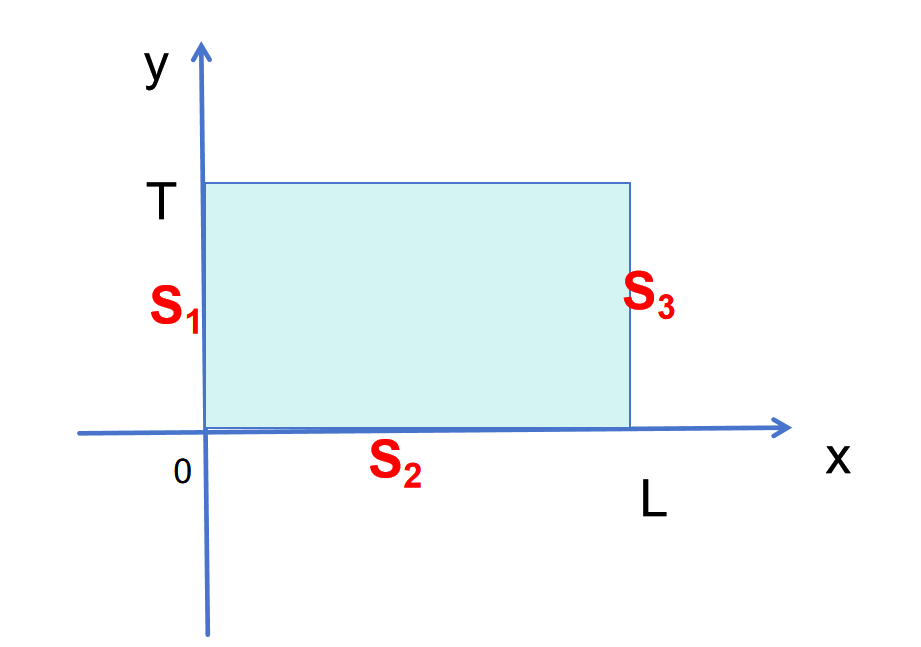
\includegraphics[width=10cm]{1.png}
	%\caption{售猪问题的净收益$f(x)$关于售猪时间$x$的曲线图}
\end{figure}

\textbf{定理1 (极值原理):} 假设函数 $ u=u(x, t) \in C^{2,1}(Q) \cap C(\overline{Q}) $ 且满足方程 (1), 那么 $ u(x, t) $ 在 $ \overline{Q} $ 上的最大值和最小值在边界 $ \Gamma $ 上可以达到, 即
$$
\max _{\overline{Q}} u(x, t)=\max _{\Gamma} u(x, t), \quad \min _{\overline{Q}} u(x, t)=\min _{\Gamma} u(x, t) .
$$

下面利用极值原理来讨论热传导方程解的唯一性和对边界及初始数据的连续依赖性 (即稳定性).

\textbf{定理2 :}初边值问题
\begin{equation*}
    \left\{\begin{array}{ll}
u_{t}=c^{2} u_{x x}+h(x, t), & 0<x<L, t>0, \\
u(x, 0)=f(x), & 0 \leqslant x \leqslant L, \\
u(0, t)=p(t), u(L, t)=q(t), & t \geqslant 0
\end{array}\right.\tag{2}
\end{equation*}
在函数空间 $ C^{2,1}(Q) \cap C(\overline{Q}) $ 中的解是唯一的, 且连续依赖初始和边界数据.

证: 先证解的唯一性. 设 $ u_{1}(x, t) $ 和 $ u_{2}(x, t) $ 是问题 (2) 在函数空间 $ C^{2,1}(Q) \cap C(\overline{Q}) $ 中的两个解. 记 $ u(x, t)=u_{1}(x, t)-u_{2}(x, t) $, 那么 $ u=u(x, t) $ 满足齐次方程和齐次初边值条件的定解问题
$$
\left\{\begin{array}{ll}
u_{t}=c^{2} u_{x x}, & 0<x<L, t>0, \\
u(x, 0)=0, & 0 \leqslant x \leqslant L, \\
u(0, t)=u(L, t)=0, & t \geqslant 0 .
\end{array}\right.
$$
对任意一点 $ \left(x_{0}, t_{0}\right), 0 \leqslant x_{0} \leqslant L, t_{0}>0 $, 记
$$
Q=\left\{(x, t) \mid 0 \leqslant x \leqslant L, 0 \leqslant t<t_{0}\right\}
$$
和 $ \Gamma $ 为 $ Q $ 的抛物边界. 那么 $ u(x, t) $ 在 $ \overline{Q} $ 上连续, 且满足
$$
u_{t}=c^{2} u_{x x}, \quad 0<x<L, 0<t \leqslant t_{0} .
$$
由定理 1 得, 对任意 $ (x, t) \in \overline{Q} $, 成立
$$
0=\min _{\Gamma} u(x, t) \leqslant u(x, t) \leqslant \max _{\overline{Q}} u(x, t)=0 .
$$
即在区域 $ \overline{Q} $ 上, $ u(x, t)=0 $. 特别地, $ u\left(x_{0}, t_{0}\right)=0 $ 和 $ u_{1}\left(x_{0}, t_{0}\right)=u_{2}\left(x_{0}, t_{0}\right) $. 由于 $ \left(x_{0}, t_{0}\right) $ 是任意的, 所以
$$
u_{1}(x, t)=u_{2}(x, t), \quad 0 \leqslant x \leqslant L, t \geqslant 0,
$$
这表明解是唯一的.

下面考虑解对初始数据和边界数据的连续依赖性. 设 $ u_{i}(x, t)(i=1,2) $ 是问题
$$
\left\{\begin{array}{ll}
u_{t}=c^{2} u_{x x}+h(x, t), & 0<x<L, t>0, \\
u(x, 0)=f_{i}(x), & 0 \leqslant x \leqslant L, \\
u(0, t)=p_{i}(t), u(L, t)=q_{i}(t), & t \geqslant 0
\end{array}\right.
$$
的解. 令 $ u(x, t)=u_{1}(x, t)-u_{2}(x, t), p(t)=p_{1}(t)-p_{2}(t), q(t)=q_{1}(t)-q_{2}(t) $, $ f(x)=f_{1}(x)-f_{2}(x) $. 则 $ u=u(x, t) $ 满足
$$
\left\{\begin{array}{ll}
u_{t}=c^{2} u_{x x}, & 0<x<L, t>0, \\
u(x, 0)=f(x), & 0 \leqslant x \leqslant L, \\
u(0, t)=p(t), u(L, t)=q(t), & t \geqslant 0 .
\end{array}\right.
$$
当 $ 0 \leqslant x \leqslant L, t \geqslant 0 $ 时, 如果有 $ |f(x)|<\varepsilon,|p(t)|<\varepsilon,|q(t)|<\varepsilon $, 那么由极值原理得 $ |u(x, t)|<\varepsilon, 0 \leqslant x \leqslant L, t \geqslant 0 $. 这就证明了初边值问题 (2) 解关于初始数据和边界数据的稳定性. 定理证毕.



\subsubsection{拉普拉斯方程的极值原理}
\textbf{定理: (极值原理) }$ \quad $ 设 $ \Omega $ 是 $ \mathbb{R}^{3} $ 中的有界区域, 边界 $ \partial \Omega $ 光滑. 如果 $ u \in $ $ C^{2}(\Omega) \cap C(\overline{\Omega}) $ 且满足
$$
\Delta u=u_{x x}+u_{y y}+u_{z z}=0, \quad(x, y, z) \in \Omega,
$$
则 $ u $ 在边界 $ \partial \Omega $ 上达到 $ \overline{\Omega} $ 上的最大值和最小值, 即
$$
\max _{\overline{\Omega}} u(x, y, z)=\max _{\partial \Omega} u(x, y, z), \quad \min _{\overline{\Omega}} u(x, y, z)=\min _{\partial \Omega} u(x, y, z)
$$
注. 设 $ u \in C^{2}(\Omega) $, 且 $ \Delta u>0 $ (或 $ \Delta u<0 $ ), 则 $ u $ 不可能在 $ \Omega $ 内达到最大 (最小) 值.


下面利用极值原理来讨论调和方程的第一边值问题解的唯一性和稳定性.

 设 $ \Omega $ 是 $ \mathbb{R}^{3} $ 中的一有界区域, 其边界 $ \partial \Omega $ 光滑. 如果泊松方程的狄利克雷内问题
$$
(1)\left\{\begin{array}{ll}
\Delta u=g(x, y, z), & (x, y, z) \in \Omega \\
u(x, y, z)=f(x, y, z), & (x, y, z) \in \partial \Omega
\end{array}\right.
$$
在函数空间 $ C^{2}(\Omega) \cap C(\overline{\Omega}) $ 中存在解, 则必唯一, 且连续依赖于边界数据.

证: 设 $ u_{1}, u_{2} $ 是问题 $ (1) $ 的两个解, 那么函数 $ u=u_{1}-u_{2} $ 满足
$$
\Delta u=0, \quad(x, y, z) \in \Omega ; \quad u(x, y, z)=0, \quad(x, y, z) \in \partial \Omega .
$$
由定理, 
$$
\max _{ \overline{\Omega}} u=\max _{ \partial \Omega} u=0, \quad \min _{ \overline{\Omega}} u=\min _{ \partial \Omega} u=0
$$
所以在 $ \Omega $ 内有 $ u=0 $, 即 $ u_{1}=u_{2} $.所以问题 (1) 的解是唯一的.
(注意到这里的 $ \Omega $ 是一个有界区域. 无界域上的边值问题, 解的唯一性不一定是对的. )

下面证明解对边界数据的稳定性.
设 $ u_{1} $ 和 $ u_{2} $ 是定解问题 (1) 分别对应于边值 $ f_{1} $ 和 $ f_{2} $ 的两个解, 则函数 $ u=u_{1}-u_{2} $ 满足
$$
\left\{\begin{array}{ll}
\Delta u=0, & (x, y, z) \in \Omega, \\
u(x, y, z)=f(x, y, z), & (x, y, z) \in \partial \Omega,
\end{array}\right.
$$
其中 $ f(x, y, z)=f_{1}(x, y, z)-f_{2}(x, y, z) $.
假定在边界 $ \partial \Omega $ 上, $ |f(x, y, z)|<\varepsilon $, 那么由定理 , 对任意 $ (x, y, z) \in \Omega $, 成立
$$
-\varepsilon<\min _{\partial \Omega}\left(f_{1}-f_{2}\right)=\min _{\partial \Omega} u \leqslant u(x, y, z) \leqslant \max _{\partial \Omega} u=\max _{\partial \Omega}\left(f_{1}-f_{2}\right)<\varepsilon .
$$
即对任意 $ (x, y, z) \in \bar{\Omega},|u(x, y, z)|<\varepsilon $. 所以定解问题 (1) 的解连续依赖于所给的边界数据. 证毕.
\subsection{热传导方程的柯西问题}
\subsubsection{齐次方程}

一维热传导方程的 Cauchy 问题是
\begin{equation*}
    u_{t}-a^{2} u_{x x}=0,-\infty<x<+\infty, t>0,\tag{1}
\end{equation*}
具有初始条件
\begin{equation*}
   \left.u\right|_{t=0}=\varphi(x), \quad-\infty<x<+\infty . \tag{2}
\end{equation*}

它的求解我们一般采用 Fourier 变换方法,在这里我们利用无量纲法推导出热传导方程的自相似解,然后我们将应用相似变换法求解 Cauchy 问题 (1), (2). 为此, 我们首先给出热传导方程 (1) 的解的如下性质. 这里就不提供证明.

性质 1. 设 $ u(x, t) $ 是 (1) 的解, 则对任意的 $ y \in \mathbf{R}, u(x-y, t) $ 也是 (1) 的解.

性质 2. 设 $ u(x, t) $ 是 (1) 的解, 则它的各阶导数 (比如 $ u_{x}, u_{t}, u_{x t}, u_{x x} $ 等) 也是 (1) 的解.

性质 3. 设 $ S(x, t) $ 是  (1) 的解, 则对任意连续函数 $ g(y) $,
$$
v(x, t)=\int_{-\infty}^{\infty} S(x-y, t) g(y) \mathrm{d} y
$$
也是 (1) 的解.
性质4. 设 $ u(x, t) $ 是 (1) 的解, 则对任意的 $ \lambda>0, u\left(\lambda x, \lambda^{2} t\right) $ 也是 (1) 的解.

由性质4 , 我们易知方程 (1) 具有如下形式的自相似解:
$$
Q(x, t)=q(\xi), \quad \xi=\frac{x}{\sqrt{t}} .
$$
经过简单的计算可知 $ q(\xi) $ 满足如下常微分方程
$$
q^{\prime \prime}+\frac{1}{2 a^{2}} \xi q^{\prime}=0
$$
其通解可通过两次积分求出:
$$
q(\xi)=c_{1} \int_{0}^{\xi} \mathrm{e}^{-\frac{1}{4 a^{2}} \eta^{2}} \mathrm{~d} \eta+c_{2},
$$
其中 $ c_{1}, c_{2} $ 是两个积分常数.
因此
$$
Q(x, t)=c_{1} \int_{0}^{\frac{x}{\sqrt{t}}} \mathrm{e}^{-\frac{1}{4 a^{2}} \eta^{2}} \mathrm{~d} \eta+c_{2}
$$
由性质2 知
$$
S(x, t)=\frac{\partial}{\partial x} Q(x, t)=\frac{c_{1}}{\sqrt{t}} \mathrm{e}^{-\frac{x^{2}}{4 a^{2} t}}
$$
是 (1) 的解, 从而由性质 3 知对任意连续函数 $ g(y) $
\begin{equation*}
    v(x, t)=\int_{-\infty}^{\infty} S(x-y, t) g(y) \mathrm{d} y=\frac{c_{1}}{\sqrt{t}} \int_{-\infty}^{\infty} \mathrm{e}^{-\frac{(x-y)^{2}}{4 a^{2} t}} g(y) \mathrm{d} y\tag{3}
\end{equation*}
也是 (1) 的解. 为了求出 Cauchy 问题 (1), (2) 的解, 我们利用初始条件 (2)确定 (3) 中的常数 $ c_{1} $.
事实上,作变换 $ y=x+2 a \sqrt{t} \eta $, 则 (3) 可改写为
$$
v(x, t)=2 a c_{1} \int_{-\infty}^{\infty} \mathrm{e}^{-\eta^{2}} g(x+2 a \sqrt{t} \eta) \mathrm{d} \eta .
$$
在该式中令 $ t \rightarrow 0^{+} $, 得
$$
\varphi(x)=v(x, 0)=2 a c_{1} \int_{-\infty}^{\infty} \mathrm{e}^{-\eta^{2}} g(x) \mathrm{d} \eta=2 \sqrt{\pi} a c_{1} g(x)
$$
因此,要使 (3)满足初始条件 (2), 必须取
$$
c_{1}=\frac{\varphi(x)}{2 \sqrt{\pi} \operatorname{ag}(x)} .
$$

将 $c_1$ 代人到 (3), 我们得到 Cauchy 问题 (1), (2) 的解为
\begin{equation*}
    u(x, t)=\frac{1}{2 a \sqrt{\pi t}} \int_{-\infty}^{\infty} \mathrm{e}^{-\frac{( x-y)^{2}}{4 a^{2} t}} \varphi(y) \mathrm{d} y .\tag{4}
\end{equation*}
我们通常称 (4) 为 Poisson 公式, 若记
$$
G(x, t)=\left\{\begin{array}{ll}
\frac{1}{2 a \sqrt{\pi t}} \mathrm{e}^{-\frac{x^{2}}{4 a^{2} t},} & t>0, \\
0, & t<0,
\end{array}\right.
$$
那么 (4) 可改写成
$$
u(x, t)=\int_{-\infty}^{\infty} G(x-y, t) \varphi(y) \mathrm{d} y .
$$
由其所确定的函数通常称为热核函数.(当然, 上面的推导完全是形式的.)

\subsubsection{非齐次方程}

我们考虑非齐次热传导方程的 Cauchy 问题
\begin{equation*}
    \left\{\begin{array}{ll}
u_{t}-a^{2} u_{x x}=f(x, t), & -\infty<x<+\infty, t>0, \\
\left.u\right|_{t=0}=\varphi(x), & -\infty<x<+\infty .
\end{array}\right.\tag{1}
\end{equation*}
由线性方程的叠加原理, (1) 的求解可分解为如下两个问题的求解
\begin{equation*}
\left\{\begin{array}{ll}
u_{t}-a^{2} u_{x x}=0, & -\infty<x<+\infty, \\
\left.u\right|_{t=0}=\varphi(x), & -\infty<x<+\infty,
\end{array}\right.\tag{2}
\end{equation*}
及
\begin{equation*}
\left\{\begin{array}{ll}
u_{t}-a^{2} u_{x x}=f(x, t), & -\infty<x<+\infty, t>0, \\
\left.u\right|_{t=0}=0, & -\infty<x<+\infty .
\end{array}\right.\tag{3}
\end{equation*}
即若 $ u_{1}(x, t), u_{2}(x, t) $ 分别是 Cauchy 问题 (2), (3) 的解, 则 $ u(x, t)=u_{1}(x, t) $ $ +u_{2}(x, t) $ 是 Cauchy 问题 (1) 的解.

Cauchy 问题 (2)的求解我们已经讨论过.下面我们用关于求解非齐次波动方程的 Duhamel 原理的方法来求解 Cauchy 问题 (3).

\textbf{引理(齐次化原理) }若函数 $ w(x, t, \tau) $ 是 Cauchy 问题
\begin{equation*}
\left\{\begin{array}{ll}
w_{t}-a^{2} w_{x x}=0, & -\infty<x<+\infty, \\
\left.w\right|_{t=r}=f(x, \tau), & -\infty<x<+\infty
\end{array}\right.\tag{4}
\end{equation*}
的解, 则函数
$$
u(x, t)=\int_{0}^{t} w(x, t, \tau) \mathrm{d} \tau
$$
就是 Cauchy 问题(3)的解.

为了应用 Poisson 公式 求解 Cauchy 问题 (4), 令 $ t^{\prime}=t-\tau $, 得如下 Cauchy 问题:
$$
\left\{\begin{array}{l}
w_{t^{\prime}}-a^{2} w_{x x}=0, \quad-\infty<x<+\infty, t^{\prime}>0 \\
\left.w\right|_{t^{\prime}=0}=f(x, \tau), \quad-\infty<x<+\infty .
\end{array}\right.
$$
易知解为
$$
w\left(x, t^{\prime}, \tau\right)=\int_{-\infty}^{\infty}=G\left(x-y, t^{\prime}\right) f(y, \tau) \mathrm{d} y .
$$
从而 (4) 的解为
\begin{equation*}
w(x, t, \tau)=\int_{-\infty}^{\infty} G(x-y, t-\tau) f(y, \tau) \mathrm{d} y .\tag{5}
\end{equation*}

由引理及 (5), 我们能获得 Cauchy 问题 (1) 的解:
$$
u(x, t)=\int_{-\infty}^{\infty} G(x-y, t) \varphi(y) \mathrm{d} y+\int_{0}^{t} \int_{-\infty}^{\infty} G(x-y, t-\tau) f(y, \tau) \mathrm{d} y \mathrm{~d} \tau .
$$

\subsection{二阶线性方程的分类}
含两个自变量的二阶线性偏微分方程的一般形式是
$$
a_{11} u_{x x}+2 a_{12} u_{x y}+a_{22} u_{y y}+b_{1} u_{x}+b_{2} u_{y}+c u=f
$$
其中 $ a_{11}, a_{12}, a_{22} $ 不同时为零. 方程的分类依赖于行列式 $ \Delta=a_{11} a_{22}-a_{12}^{2} $ 的取值或矩阵 $ A=\left(\begin{array}{ll}a_{11} & a_{12} \\ a_{21} & a_{22}\end{array}\right) $ 的特征值 $ \lambda_{1}, \lambda_{2} $ 的符号.

若 $ \Delta>0 $ (等价地, $ \lambda_{1}, \lambda_{2} $ 不等于零且同号), 则称方程 为椭圆型的;

若 $ \Delta<0 $ (等价地, $ \lambda_{1}, \lambda_{2} $ 不等于零且异号), 则称方程 为双曲型的;

若 $ \Delta=0 $ (等价地, $ \lambda_{1}, \lambda_{2} $ 有一个为零), 则称方程  为抛物型的.
\newpage
\section{数学物理方程模拟题}
\subsection{模拟题参考答案}
1. 偏微方程只给出初始条件时称为\textbf{初值}问题.

2. 解的\textbf{存在、唯一性和稳定性}称为问题的适定性.

3. 三维 Laplace 方程的基本解是
$
v=-\dfrac{1}{4 \pi r}=-\dfrac{1}{4 \pi \sqrt{\left(x-x_{0}\right)^{2}+\left(y-y_{0}\right)^{2}+\left(z-z_{0}\right)^{2}}}.
$

4. 二维齐次热传导方程的一般形式为$ u_t = a^2(u_{xx} +u_{yy})$.

5. $ u_{t}-\left(u_{x x}+u_{y y}\right)=0 $ 是\textbf{抛物型}偏微分方程.

6. 说明物理现象初始状态的条件叫\textbf{初始条件} , 说明边界约束情况的条件叫\textbf{边界条件}.

7.边界条件 $ \left.\left(\frac{\partial u}{\partial n}+\sigma u\right)\right|_{\partial \Omega}=f $ 是\textbf{第三类}边界条件, 其中 $ \partial \Omega $ 为边界.

\begin{questions}

\question{
下列不是调和函数的是 ( )

A. $ u(x, y)=e^{x} \sin y $

B. $ u(x, y)=x^{2}+y^{2} $

C. $ u(x, y)=a x+b y+c $

D. $ u(x, y)=x^{3}-3 x y^{2} $
}
\begin{solution}
   我们可以使用拉普拉斯算子 $\Delta u$ 来验证哪个函数是调和函数。调和函数满足 $\Delta u = 0$。让我们使用 $\Delta u$ 来验证每个选项:

A. $u(x, y) = e^x \sin y$:
$$\Delta u = \frac{\partial^2 u}{\partial x^2} + \frac{\partial^2 u}{\partial y^2} = e^x \sin y - e^x \sin y = 0$$

由于 $\Delta u$ 等于零,所以 A 是调和函数。

B. $u(x, y) = x^2 + y^2$:
$$\Delta u = \frac{\partial^2 u}{\partial x^2} + \frac{\partial^2 u}{\partial y^2} = 2 + 2 = 4$$

由于 $\Delta u$ 不等于零,所以 B 不是调和函数。

C. $u(x, y) = ax + by + c$:
$$\Delta u = \frac{\partial^2 u}{\partial x^2} + \frac{\partial^2 u}{\partial y^2} = 0$$

由于 $\Delta u$ 等于零,所以 C 是调和函数。

D. $u(x, y) = x^3 - 3xy^2$:
$$\Delta u = \frac{\partial^2 u}{\partial x^2} + \frac{\partial^2 u}{\partial y^2} = 6x - 6x = 0$$

由于 $\Delta u$ 等于零,所以 D 也是调和函数。

因此A, C ,D 都是调和函数,只有 B 不是调和函数。
\end{solution}
\question{
设 $ G\left(M, M_{0}\right) $ 为区域 $ \Omega $ 上 Laplace 方程 $ \Delta u=0 $ Dirichlet 问题的 Green 函数,
则 $$ \iint_{\partial \Omega} \frac{\partial G\left(M, M_{0}\right)}{\partial \vec{\boldsymbol n}} d S_{M}=(\quad) $$

$$\mathrm{A}. 0\quad\quad\quad\quad \mathrm{B}. 1\quad\quad\quad\quad \mathrm{C}. -1\quad\quad\quad\quad \mathrm{D}.\text{不确定}$$

}
\begin{solution}
   狄利克雷问题 
$$\left\{\begin{array}{l}\Delta u=0,(x, y, z) \in \Omega \\ \left.u\right|_{\partial \Omega}=\varphi(M), M \in \partial \Omega\end{array}\right. $$
的解可表示为 
$$ u\left(M_{0}\right)=-\iint_{\partial \Omega} \varphi(M) \cdot \frac{\partial G\left(M, M_{0}\right)}{\partial n} d S_{M} $$
显然 $ u \equiv 1 $ 是如下边值问题
$$
\begin{array}{l}
\left\{\begin{array}{l}
\Delta u=0 \quad M \in \Omega\\
\left.u\right|_{\partial \Omega}=1
\end{array} \right.
\end{array} 
$$
的解.为此取$\varphi(M)=1$即得
$$
\iint_{\partial \Omega} \frac{\partial G\left(M, M_{0}\right)}{\partial n} d S_{M}=-1
$$
\end{solution}
\question{
考虑常微分方程特征值问题
$$
\begin{array}{l}
\dfrac{d^{2} X(x)}{d x^{2}}+\lambda X(x)=0,0<x<\pi, \\
X(0)=0, X(\pi)=0,
\end{array}
$$
不是该问题的特征值的是 ( )
$$\mathrm{A}. 1\quad\quad\quad\quad \mathrm{B}. 3\quad\quad\quad\quad \mathrm{C}. 4\quad\quad\quad\quad \mathrm{D}.16$$
}
\begin{solution}
求解特征值和特征函数的问题:
$$
\left\{\begin{array}{l}
X^{\prime \prime}+\lambda X=0 \\
X(0)=0, X(\pi)=0
\end{array} .\right.
$$
为了求解这个特征值问题, 需要分下面三种情形讨论:

1. 当 $ \lambda<0 $ 时, 方程 $ X^{\prime \prime}+\lambda X=0 $ 的通解为
$$
X(x)=A \mathrm{e}^{\sqrt{-\lambda} x}+B \mathrm{e}^{-\sqrt{-\lambda} x}
$$
其中, $ A, B $ 为两个任意常数. 代入边界条件, 得
$$
X(0)=A \cdot 1+B \cdot 1=0, \quad X(\pi)=A \mathrm{e}^{\sqrt{-\lambda} \pi}+B \mathrm{e}^{-\sqrt{-\lambda} \pi}=0
$$
因为
$$
\left|\begin{array}{cc}
1 & 1 \\
\mathrm{e}^{\sqrt{-\lambda }\pi}& \mathrm{e}^{-\sqrt{-\lambda } \pi}
\end{array}\right| \neq 0,
$$
故 $ A=B=0 $, 即有 $ X(x) \equiv 0 $.
所以, 当 $ \lambda<0 $ 时, 方程 $ X^{\prime \prime}+\lambda X=0 $ 的边值问题只有零解.

2. 当 $ \lambda=0 $ 时, 方程 $ X^{\prime \prime}+\lambda X=0 $ 的通解为 $ X=A x+B $. 其中 $ A, B $ 为两个任意常数. 代入边界条件, 得
$$
X(0)=A \cdot 0+B=0, X(\pi)=A \cdot \pi+B=0 .
$$
从而 $ A=B=0 $. 此时, 方程 $ X^{\prime \prime}+\lambda X=0 $ 的边值问题也只有零解.

3. 当 $ \lambda>0 $ 时, 方程 $ X^{\prime \prime}+\lambda X=0 $ 的通解为
$$
X(x)=A \cos \sqrt{\lambda} x+B \sin \sqrt{\lambda} x .
$$
代入边界条件, 得
$$
X(0)=A \cdot 1+B \cdot 0=0, \quad X(L)=A \cos \sqrt{\lambda} \pi+B \sin \sqrt{\lambda} \pi=0 .
$$
即 $ A=0, B \sin \sqrt{\lambda} \pi=0 $. 为了使 $ X(x) $ 不恒为零, 应有 $ B \neq 0 $, 即 $ \sin \sqrt{\lambda} \pi=0 $. 于是, 得 $ \sqrt{\lambda} \pi=k \pi, k=1,2, \cdots $. 满足这等式的 $ \lambda $ 值就是特征值, 记为 $ \lambda_{k}: $
$$
\lambda_{k}=k^{2} , k=1,2, \cdots
$$
因此$\lambda$可以取1,4,9,而不可能为3.
\end{solution}
\question{
设 $ u $ 是单位圆盘 $ \Omega $ 上的调和函数, 则其在 $ \overline{\Omega} $ 上的最大值不可能在点( )达到
$$ \mathrm{A.}(0,0) \quad\quad\quad\quad \mathrm{B.}(0,1)  \quad\quad\quad\quad\mathrm{C.}(1,0)\quad\quad\quad\quad  \mathrm{D.}(-1,0) $$
}
\begin{solution}
    $ \mathbb{R}^{n} $ 中一个有界区域 $ \Omega $ 上的调和函数一定在边界 $ \partial \Omega $ 上达到 $ \overline{\Omega} $ 上的最大值和最小值, 即
$$
\max _{x \in \overline{\Omega}} u=\max _{x \in \partial \Omega} u, \quad \min _{x \in \overline{\Omega}} u=\min _{x \in \partial \Omega} u .
$$

根据调和函数的上述性质,如果 $u$ 是单位圆盘 $\Omega$ 上的调和函数,则 $u$ 在 $\overline{\Omega}$上的最大值只能出现在 $\partial \Omega$ 上。因此在平面的圆周上的任意一点均有可能取最大值,而在圆内的点(0,0)上不可能取到最大值.

因此,在选项中,最大值不可能出现在点 $(0,0)$ (选项 A)
\end{solution}

\question{
一维波动方程初值问题
$$
\left\{\begin{array}{ll}
u_{t t}-u_{x x}=0,&-\infty<x<\infty, \\
u(x, 0)=\sin x, u_{t}(x, 0)=0,&-\infty<x<\infty,
\end{array}\right.
$$
解为 ( )

$$ \begin{array}{llll}\mathrm{A.} \sin x \cos t & \mathrm{~B.} \sin x \sin t & \mathrm{C.} \frac{\sin x \cos t}{2} & \mathrm{D.} 2 \sin x \sin t\end{array} $$
}
\begin{solution}
    根据达朗贝尔公式
$$
u(x, t)=\frac{1}{2}[\varphi(x+a t)+\varphi(x-a t)]+\frac{1}{2 a} \int_{x-a t}^{x+a t} \psi(\xi) d \xi
$$
由题意 $ a=1 . \quad \varphi(x)=\sin x , \psi(x)=0$.
即
$$u(x, t)=\frac{1}{2}[\sin (x+t)+\sin (x-t)]=\sin x\cdot\cos t \text { (积化和差公式) }$$
\end{solution}
\end{questions}

\begin{questions}
\question{
 求解齐次波动方程初值问题
$$
\left\{\begin{array}{l}
u_{t t}-a^{2} u_{x x}=0,-\infty<x<\infty, \\
u(x, 0)=\sin x, u_{t}(x, 0)=\cos x,-\infty<x<\infty .
\end{array}\right.
$$
}
\begin{solution}
直接利用达朗贝尔公式
$$
\begin{aligned}
u(x, t) & =\frac{1}{2}[\sin (x+a t)+\sin (x-a t)]+\frac{1}{2 a} \int_{x-a t}^{x+a t} \cos \xi d \xi \\
& =\sin x \cdot \cos a t+\left.\frac{1}{2 a} \sin \xi\right|_{x-a t} ^{x+a t} \\
& =\sin x \cdot \cos a t+\frac{1}{2 a}[\sin (x+a t)-\sin (x-a t)] \\
& =\sin x \cdot \cos a t+\frac{1}{a} \cos x \sin a t
\end{aligned}
$$
\end{solution}
\question{ 求解非齐次波动方程的初值问题
$$
\begin{array}{l}
u_{t t}-a^{2} u_{x x}=2 x t,-\infty<x<\infty, t>0, \\
u(x, 0)=x^{2}, u_{t}(x, 0)=\sin 2 x .
\end{array}
$$}
\begin{solution}
    直接利用一维非齐次波动方程的初值问题的解表达式,有
$$
\begin{aligned}
& u(x, t)=\frac{1}{2}[\varphi(x+a t)+\varphi(x-a t)]+\frac{1}{2 a} \int_{x-a t}^{x+a t} \psi(\xi) d \xi \\
+ & \frac{1}{2 a} \int_{0}^{t} \int_{x-a(t-\tau)}^{x+a(t-\tau)} f(\xi, \tau) d \xi d \tau \\
= & \frac{1}{2}\left[(x+a t)^{2}+(x-a t)^{2}\right]+\frac{1}{2 a} \int_{x-a t}^{x+a t} \sin 2 \xi d \xi \\
+ & \frac{1}{2 a} \int_{0}^{t} \int_{x-a(t-\tau)}^{x+a(t-\tau)} 2 \xi \tau d \xi d \tau \\
= & x^{2}+a^{2} t^{2}+\frac{1}{2 a} \sin 2 x \sin 2 a t+\frac{1}{3} x t^{3}
\end{aligned}
$$

\hrule

具体分析:

上述问题中的方程和定解条件都是线性的所以根据叠加原理,将上述定解问题分解为以下两个定解问题:

$$(1) \left\{\begin{array}{l}u_{t t}-a^{2} u_{x x}=0 \\ u(x, 0)=x^{2}, u_{t}(x, 0)=\sin 2 x\end{array}\right. $$
$$(2) \left\{\begin{array}{l}u_{t t}-a^{2} u_{x x}=2 x t \\ u(x, 0)=0, u_{t}(x, 0)=0\end{array}\right. $$
令$u=u_{1}(x, t)+u_{2}(x, t)$

对于问题(1),我们利用达朗贝公式求解
$$
\begin{aligned}
u(x, t) & =\frac{1}{2}[u(x+a t)+v(x-a t)]+\frac{1}{2 a} \int_{x-a t}^{x+a t} \psi(\xi) d \xi \\
& =\frac{1}{2}\left[(x+a t)^{2}+(x-a t)^{2}\right]+\frac{1}{2 a} \int_{x-a t}^{x+a t} \sin 2 \xi d \xi \\
& =x^{2}+a^{2} t^{2}+\left.\frac{1}{2 a}\left(-\frac{1}{2} \cos 2 \xi\right)\right|_{x-a t} ^{x+a t} \\
& =x^{2}+a^{2} t^{2}-\frac{1}{4 a}[\cos (2 x+2 a t)-\cos (2 x-2 a t)] \\
& =x^{2}+a^{2} t^{2}+\frac{1}{2 a} \sin 2 x \cdot \sin 2 a t \quad \text { (积化和差公式) }
\end{aligned}
$$

对于问题 (2)我们利用齐次化原理求解, 由齐次化原理
$$
 u_{2}(x, t)=\int_{0}^{t} w(x, t, \tau) d \tau
$$
其中 $ w(x, t, \tau) $ 是  
$$ (3) \left\{\begin{array}{l}w_{t t}=a^{2} \omega_{x x}, t>\tau \\ \left.w\right|_{t=\tau}=0 \\ \left.w_{t}\right|_{t=\tau}=f(x, \tau)=2 x \tau\end{array}\right. $$
的解

令 $ y=t-\tau $, 则定解问题(3) 化为
$$
\left\{\begin{array}{l}
w_{t t}=a^{2} w_{y y} \\
w_{y=0}=0 \leftarrow \text { 对应 } \varphi(x) \\
\left.w_{t}\right|_{y=0}=2 x \tau \leftarrow \text { 对应 } \psi(x)
\end{array}\right.
$$
由达朗贝尔公式
$$
\begin{aligned}
w(x, t, \tau) & =\frac{1}{2}[\varphi(x+a t)+\varphi(x-a t)]+\frac{1}{2 a} \int_{x-a y}^{x+a y} f(\xi, \tau) d \xi \\
& =\frac{1}{2 a} \int_{x-a \mid t-\tau)}^{x+a(t-\tau)} 2 \xi \tau d \xi
\end{aligned}
$$
则 
$$
\begin{aligned}
 u_{2}(x, t)&=\frac{1}{2 a} \int_{0}^{t} \int_{x-a(t-\tau)}^{x+a(t-\tau)} 2 \xi \tau d \xi d \tau \\
&=\left.\frac{1}{2 a} \int_{0}^{t} \tau \cdot \xi^{2}\right|_{x-a(t-\tau)} ^{x+a(t-\tau)} d \tau \\
&=\frac{1}{2 a} \int_{0}^{t} 4 a x(t-\tau) \cdot \tau d \tau \\
&=2x \int_{0}^{t}\left(t \tau-\tau^{2}\right) d \tau \\
&=2\left.x\left(\frac{1}{2} t \tau^{2}-\frac{1}{3} \tau^{3}\right)\right|_{0} ^{t} \\
&=2x\left(\frac{1}{2} t^{3}-\frac{1}{3} t^{3}\right)=\frac{1}{3} x t^{3}
\end{aligned}
$$
因此 $ u(x, t)=u_{1}(x, t)+u_{2}(x, t) $
$$
\begin{aligned}
u(x,t) & =u_{1}(x, t)+u_{2}(x, t) \\
& =x^{2}+a^{2} t^{2}+\frac{1}{3} x t^{3}+\frac{1}{2 a} \sin 2 x \sin 2 a t
\end{aligned}
$$

\end{solution}
\question{
用分离变量法求解如下热传导方程初边值问题
$$
\left\{\begin{array}{l}
u_{t}-a^{2} u_{x x}=0,0<x<l, t>0, \\
u(0, t)=u(l, t)=0, \\
u(x, 0)=\cos x .
\end{array}\right.
$$
}
\begin{solution}
    先求满足方程和边条件的分离变量形如:
$$
u(x, t)=X(x) \cdot T(t)
$$
的非零解. 其中 $ X(x), T(t) $ 为待定函数.
把$u(x,t)$代入方程 $u_{t}-a^{2} u_{x x}=0$  得
$$
X(x) T^{\prime}(t)=a^{2} X^{\prime \prime}(x) T(t),
$$
即 
$$\frac{T^{\prime}(t)}{a^{2} T(t)}=\frac{X^{\prime \prime}(x)}{X(x)}=-\lambda $$

由于上式左端与 $ x $ 无关,而右端与 $ t $ 无关, 故它为常数. 用 $ -\lambda $表示它, 于是得两个常微分方程:
$$
\begin{array}{c}
T^{\prime}(t)+a^{2} \lambda T(t)=0, \\
X^{\prime \prime}(x)+\lambda X(x)=0
\end{array}
$$
通过解两个常微分方程来决定 $ T(t), X(x) $.  代入初始条件得:
$$
\begin{array}{l}
u(0, t)=X(0) T(t)=0 \\
u(l, t)=X(l) T(t)=0 .
\end{array}
$$
因为求非零解, 故 $ T(t) \neq 0 $, 因此得
$$
X(0)=X(l)=0
$$
(i) 先求如下问题的解:
$$
\left\{\begin{array}{l}
X^{\prime \prime}(x)+\lambda X(x)=0, \\
X(0)=X(l)=0 .
\end{array}\right.
$$
方程$X^{\prime \prime}(x)+\lambda X(x)=0$的通解依赖 $ \lambda $ 的取不同值而不同, 下面分三种情况讨论 $ \lambda $.

当 $ \lambda \leqslant 0 $ 时, 无非零解 .

当 $ \lambda>0 $ 时, 通解为
$$
X(x)=C_{1} \cos \sqrt{\lambda} x+C_{2} \sin \sqrt{\lambda} x
$$
同时又满足初始条件时, 则得:
$$
\begin{array}{c}
X(0)=C_{1}=0, \\
X(l)=C_{2} \sin \sqrt{\lambda} l=0, \text { 即 } C_{2} \sin \sqrt{\lambda} l=0 .
\end{array}
$$

当 $ C_{2} \neq 0 $ 时, 则 $ \sin \sqrt{\lambda} l=0 $,
$$
\sqrt{\lambda} l=k \pi,
$$
特征值为:
$$
\lambda_{k}=\left(\frac{k \pi}{l}\right)^{2} \quad k=1,2 \cdots,
$$
其对应解:
$$
X_{k}(x)=C_{k} \sin \frac{k \pi}{l} x 
$$

(ii) 再解如下方程:
$$
T^{\prime}(t)+\lambda a^{2} T(t)=0,
$$
即
$$
\begin{array}{l}
\frac{T^{\prime}(t)}{T(t)}=-\lambda a^{2} \\
\frac{d T}{T}=-\lambda a^{2} d t
\end{array}
$$
两边取积分得:

因此:
$$
\begin{array}{c}
\ln T=-\lambda a^{2} t+\ln C, \text { 即 } \\
T(t)=C e^{-\lambda a^{2} t} .
\end{array}
$$
$$
T_{k}(t)=C_{k} e^{-\lambda a^{2} t} .
$$
于是得到满足方程及初始条件的非零特解
$$
u_{k}(x, t)=X_{k}(x) T_{k}(t)=A_{k} e^{-\left(\frac{k \pi a}{l}\right)^{2} t} \sin \frac{k \pi}{l} x .
$$
再求混合问题的解

一般说来, 上述形式的特解中任何一个不一定能满足初条件 $u(x, 0)=\cos x$ . 为了满足任意给定的初值, 应当把所有可能的特解迭加起来成为函数项级数.
$$
u(x, t)=\sum_{k=1}^{\infty} u_{k}(x, t)=\sum_{k=1}^{\infty} A_{k} e^{-\left(\frac{k \pi a}{l}\right)^{2}} \sin \frac{k \pi x}{l},
$$
其中 $ A_{k} $ 是待定的.
当 $ t=0 $ 时,$ u(x, 0)=\cos x $,
当 $ \varphi(x) $ 在 $ [0, l] $ 上能展开正弦 Fourier 级数时, 则得
$$
\sum_{k=1}^{\infty} A_{k} \sin \frac{k \pi x}{l} \sim \cos x ,
$$
其中 $ A_{k}=\frac{2}{l} \int_{o}^{l} \cos x  \sin \frac{k \pi x}{l} d x $.
\end{solution}
\question{
$ \Omega=\left\{(x, y) \in \mathbb{R}^{2} \mid 0<x<1,0<y<1\right\}, u \in C^{2}(\overline{\Omega}), \Delta u=0 $ 在 $ \overline{\Omega} $ 中, $ \left.u\right|_{x=0}=\left.u\right|_{x=1}=0 $, 当 $ 0 \leq y \leq 1 $ 时.
问函数 $ g(y)=\int_{0}^{1} u^{2}(x, y) d x $ 在开区间 $ (0,1) $ 内部是否有拐点?
}
\begin{solution}
    让我们首先求函数 $g(y)$ 的二阶导数,利用莱布尼茨积分法则,我们可以将积分和求导的顺序交换,结合链式法则得到:
$$\frac{d g(y)}{d y}=\frac{d}{d y} \int_{0}^{1} u^{2}(x, y) d x=\int_{0}^{1}( 2 u \cdot u_{y}) d x $$

$$\frac{d^{2} g(y)}{d y^{2}}=\frac{d}{d y} \int_{0}^{1} 2 u \cdot u_{y} d x=2 \int_{0}^{1} (u_{y}^{2}+u u_{y y} )dx$$


由于 $u \in C^{2}(\overline{\Omega})$ 且 $\Delta u = 0$,我们可以对 $u^2$ 应用拉普拉斯算子:
$$ \begin{array}{l} \Delta\left(u^{2}\right)=\left(u^{2}\right)_{x x}+\left(u^{2}\right)_{y y} \\ =2 u_{x}^{2}+2u u_{x x}+2 u_{y}^{2}+2u u_{y y} \\ =2\left(u_{x}^{2}+u_{y}^{2}\right)+2u\left(u_{x x}+u_{y y}\right) \\ =2|\nabla u|^{2}+2u \Delta u \\ =2|\nabla u|^{2} \\\end{array} $$
因此,$g(y)$ 的二阶导数变为:
$$ \begin{aligned} \frac{d^{2} g(y)}{d y^{2}}&=2 \int_{0}^{1} (u_{y}^{2}+u u_{y y}) d x \\& =2 \int_{0}^{1}\left[\left(u_{x}^{2}+u_{y}^{2}\right)+u\left(u_{x x}+u_{y y}\right)-\left(u_{x}^{2}+u u_{x x}\right)\right] d x \\ & =2 \int_{0}^{1}|\nabla u|^{2} d x-2 \int_{0}^{1}\left(u_{x}^{2}+u u_{x x}\right) d x \\  & =2 \int_{0}^{1}|\nabla u|^{2} d x-2 \left.u u_{x} \right|_{x=0} ^{x=1} \\ & =2 \int_{0}^{1}|\nabla u|^{2} d x>0 .\end{aligned} $$

现在,让我们分析开区间 $(0,1)$ 是否存在拐点。拐点发生在二阶导数改变符号的地方。由于 $g(y)$ 的二阶导数始终非负(因为它是梯度平方的积分),故在开区间 $(0,1)$ 内部没有拐点。
\end{solution}
\question{
求三维调和方程在上半空间上的 Dirichlet 问题
$$
\left\{\begin{array}{l}
\Delta u=u_{x x}+u_{y y}+u_{z z}=0, z>0, \\
u(x, y, 0)=f(x, y),
\end{array}\right.
$$
的解.
}
\begin{solution}
    先求半空间 $ z>0 $ 上的格林函数. 在半空间 $ z>0 $ 上任取一点 $ M_{0}=M_{0}\left(x_{0}, y_{0}, z_{0}\right) $, 在其上放置一单位正电荷, 它在无穷空间形成电场, 在上半空间任一点 $ M(x, y, z) $ 处的电位为 $ \frac{1}{4 \pi r_{M M_{0}}} $. 然后找出 $ M_{0} $ 关于边界 $ z=0 $ 的对称点 $ M_{1}=M_{1}\left(x_{0}, y_{0},-z_{0}\right) $, 并在其上放置一单位负电荷. 则它与 $ M_{0} $点的单位正电荷所产生的电位在平面 $ z=0 $ 上电位互相抵消 (如图 ).
    
因为 $ \frac{1}{4 \pi r_{M M_{1}}} $ 在 $ z>0 $ 上为调和函数, 在区域 $ z> 0 $ 上具有一阶偏导数, 故
$$
G\left(M, M_{0}\right)=\frac{1}{4 \pi}\left(\frac{1}{r_{M M_{0}}}-\frac{1}{r_{M M_{1}}}\right)
$$

便是半空间 $ z>0 $ 上的格林函数, 其中
$$
\begin{aligned}
r_{M M_{0}} & =\sqrt{\left(x-x_{0}\right)^{2}+\left(y-y_{0}\right)^{2}+\left(z-z_{0}\right)^{2}}, \\
r_{M M_{1}} & =\sqrt{\left(x-x_{0}\right)^{2}+\left(y-y_{0}\right)^{2}+\left(z+z_{0}\right)^{2}} .
\end{aligned}
$$

下面我们来计算 $ \frac{\partial G}{\partial n} $. 因为在平面 $ z=0 $ 上的外法线方向是 $ z $ 轴的负方向, 所以
$$
\left.\frac{\partial G}{\partial n}\right|_{z=0}=-\left.\frac{\partial G}{\partial z}\right|_{z=0}=-\frac{1}{2 \pi} \frac{z_{0}}{\left[\left(x-x_{0}\right)^{2}+\left(y-y_{0}\right)^{2}+z_{0}^{2}\right]^{3 / 2}} .
$$

由解的积分表达式 , 得定解问题 的形式解为
$$
u\left(M_{0}\right)=u\left(x_{0}, y_{0}, z_{0}\right)=\frac{z_{0}}{2 \pi} \int_{\infty}^{\infty} \int_{\infty}^{\infty} \frac{f(\xi, \eta) \mathrm{d} \xi \mathrm{d} \eta}{\left[\left(\xi-x_{0}\right)^{2}+\left(\eta-y_{0}\right)^{2}+z_{0}^{2}\right]^{3 / 2}}
$$
\end{solution}
\begin{figure}[h]%浮动体
	\centering
	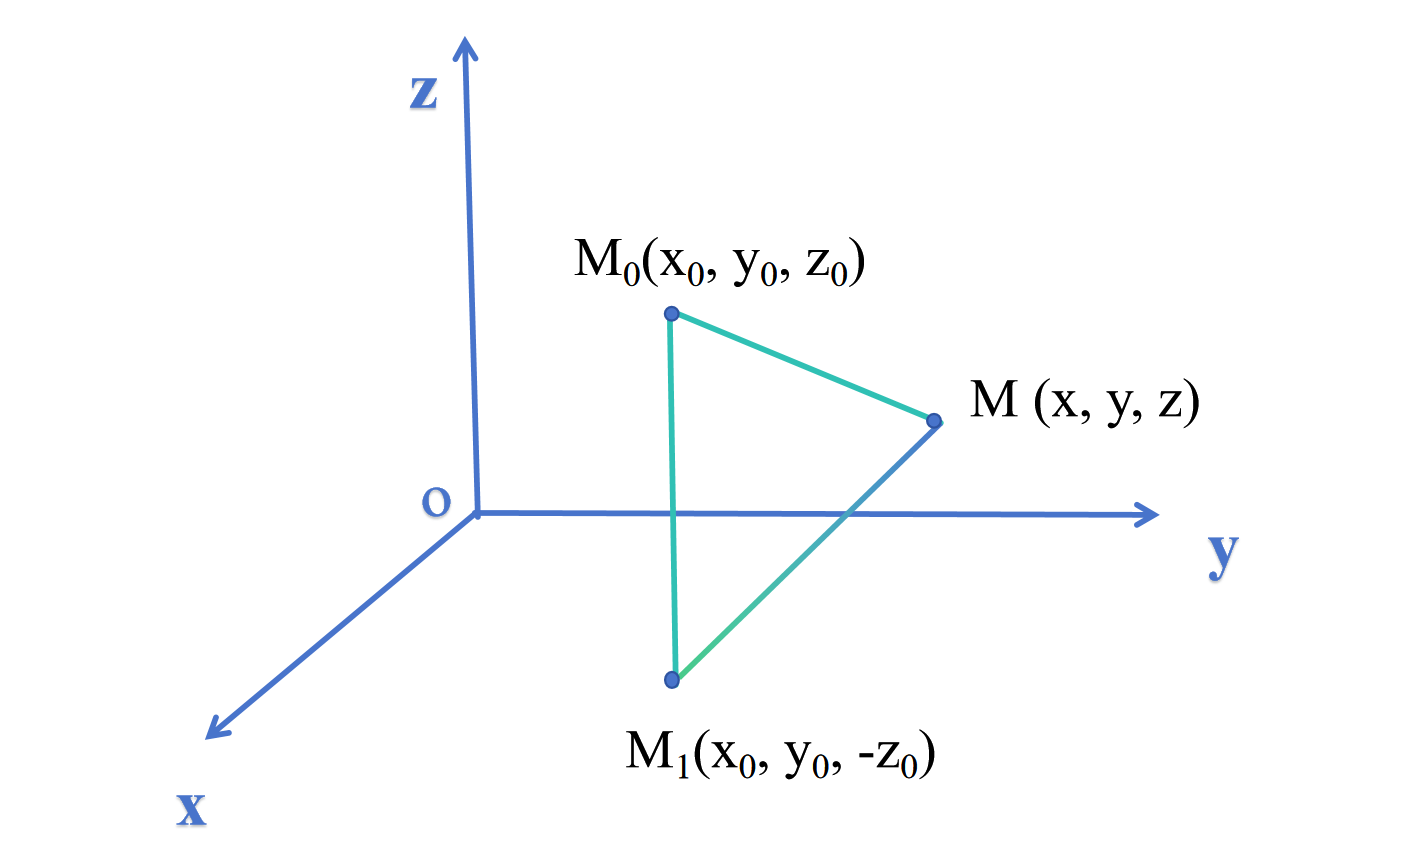
\includegraphics[width=10cm]{pic1.png}
	%\caption{售猪问题的净收益$f(x)$关于售猪时间$x$的曲线图}
\end{figure}
\question{
证明如下方程初边值问题
$$
\left\{\begin{array}{l}
u_{t}=u_{x x}+u, \quad 0<x<l, t>0, \\
u(0, t)=\mu_{1}(t), u(l, t)=\mu_{2}(t), t>0, \\
u(x, 0)=\varphi(x),
\end{array}\right.
$$
解的唯一性与对初值的连续依赖性.
}
\begin{solution}
    作变换 $ v(x, t)=e^{-t} \cdot u(x, t) $ 则 $ v(x, t) $ 满足
$$
\left\{\begin{array}{l}
v_{t}=v_{x x} \quad 0 < x < l, t>0 \\
v(x, 0)=\varphi(x) \quad 0 < x < l \\
v(0, t)=e^{-t} \cdot \mu_{1}(t), v(1, t)=e^{-t} \cdot \mu_{2}(t)
\end{array}\right.
$$

不妨设 $ v_{1}(x, t) , v_{2}(x, t) $ 是该问题的两个解记 $ v(x, t)=v_{1}(x, t)-v_{2}(x, t) $ ,那么 $ v(x, t) $ 满足齐次初边值条件的定解问题
$$
\begin{array}{l}
\left\{\begin{array}{l}
v_{t}=v_{x x} \quad 0 < x < l, t>0 \\
v(x, 0)=0 \quad 0 < x < l \\
v(0, t)=v(l, t)=0 . \quad t > 0 .
\end{array}\right. \\
\end{array}
$$
 对任意一点 $\left(x_{0}, t_{0}\right), \quad 0 \leq x_{0} \leq l, t_{0}>0$
记 $Q=\left\{(x, t) \mid 0 \leqslant x \leqslant l,0 \leqslant t \leqslant t_{0}\right\}$ 其抛物边界为 $ \Gamma $
那么 $ v(x, t) $ 在在 $ \overline{Q} $ 上连续,且满足 $ v_{t}=v_{x x}, 0< x < l , 0 < t \leqslant t_{0} $
由极值原理, 对 $ \forall(x, t) \in \overline{Q} $, 成立如下:
$$
0=\min _{\Gamma} v(x, t) \leqslant v(x, t) \leqslant \max _{\overline{Q}} v(x, t)=0
$$

即在区域 $ \overline{Q} 上, v(x, t)=0 $
特别地 $ v\left(x_{0}, t_{0}\right)=0 \Rightarrow v_{1}\left(x_{0}, t_{0}\right)=v_{2}\left(x_{0}, t_{0}\right) $ ,由于 $ \left(x_{0}, t_{0}\right) $ 是任意的
所以 $ v_{1}(x, t)=v_{2}(x, t) \quad 0 < x < l, t>0 $.
故 $ v(x, t) $ 唯一,也即 $ u(x, t) $ 唯一。

下面考虑解对初值的连续依赖性:

设 $v_{i}(x, t) $ ,$i=1,2$ 是下面问题 
$$\left\{\begin{array}{l}v_{t}=v_{x x} \\ v(x, 0)=\varphi_{i}(x) \\ v(0, t)=e^{-t} \mu_{1}^{(i)}(t), v(l, t)=e^{-t} \mu_{2}^{(i)}(t)\end{array}\right. $$
的解,令 $ v(x, t)=v_{1}(x, t)-v_{2}(x, t) $. $ \varphi(x)=\varphi_{1}(x)-\varphi_{2}(x) $.
$$
f(t)=e^{-t}\left(\mu_{1}^{(1)}(t)-\mu_{1}^{(2)}(t)\right) \quad g(t)=e^{-t}\left(\mu_{2}^{(1)}(t)-\mu_{2}^{(2)}(t)\right)
$$

那么由极值原理得 
$$|v(x, t)|< \varepsilon ,|u(x, t)|= \left|v(x, t) \cdot e^{t}\right|<\varepsilon e^{t} $$
即得证.

\end{solution}
\end{questions}


\subsection{补充内容}

1. 偏微分方程只给出初始条件而没有给出边界条件时,通常称为初值问题(Initial Value Problem,简称IVP)。在这种问题中,你需要通过给定的初始条件找到方程的解。

2. 解的存在、唯一性和稳定性通常被称为问题的适定性。这些属性是用来评估偏微分方程问题是否具有良好的解性质的重要因素。存在性指的是是否存在解,唯一性指的是解是否唯一,稳定性指的是解在输入条件的小变化下是否保持稳定。

3. 设 $ M_{0}=M_{0}\left(x_{0}, y_{0}, z_{0}\right) $ 是空间 $ \mathbb{R}^{3} $ 中某一固定点, $ M=M(x, y, z) $ 是 $ \mathbb{R}^{3} $ 中的动点, 定义函数
$$
v=-\frac{1}{4 \pi r_{M M_{0}}}=-\frac{1}{4 \pi \sqrt{\left(x-x_{0}\right)^{2}+\left(y-y_{0}\right)^{2}+\left(z-z_{0}\right)^{2}}}
$$
这里 $ r_{M M_{0}} $ 表示空间 $ M_{0} $ 与 $ M $ 两点之间的距离.

4. 二维齐次热传导方程的一般形式如下:
$$ u_t = a^2(u_{xx} +u_{yy})$$
在这个方程中,$u$ 是温度分布随时间和空间坐标 $(x, y)$ 的函数,$u_{t}$ 表示温度随时间的变化率,$a^2$ 是热传导系数,$u_{xx}$ 和 $u_{yy}$ 分别表示温度在 $x$ 和 $y$ 方向上的二阶空间导数。这方程描述了热传导过程,其中热量以时间 $t$ 为变量在空间中传导。热传导方程通常用来描述热传导过程中温度分布的演化。它可以通过适当的边界条件和初始条件来解决,以确定在给定时间和空间位置的温度分布。

5. $ u_{t}-\left(u_{xx}+u_{yy}\right)=0 $ 是类型为抛物型的偏微分方程。抛物型偏微分方程通常与时间和空间的二阶导数相结合,通常用于描述稳态或伪稳态过程,如热传导和扩散。这种类型的方程通常具有初始条件和边界条件,以唯一确定解的行为。

6. 物理现象初始状态的条件通常称为初始条件,而说明边界约束情况的条件通常称为边界条件。

初始条件是在时间 $t = 0$ 时对系统的状态或参数进行描述,它们提供了问题的初始时刻的信息。在偏微分方程问题中,初始条件通常是关于时间 t 的解函数及其导数的函数值。

边界条件是在空间中指定系统的行为或性质,通常在问题的边界或边界附近提供。它们约束了问题的解在空间域的边界上的行为,确保解在边界处满足特定条件,如固定值、导数值或其他物理条件。

这两种条件通常结合在一起,以唯一确定偏微分方程问题的解。

7. 边界条件 
$$ \left.\left(\frac{\partial u}{\partial n}+\sigma u\right)\right|_{\partial \Omega}=f $$
是第三类边界条件, 其中 $ \partial \Omega $ 为边界.

在这个条件中,$ \frac{\partial u}{\partial n} $ 表示相对于边界法向量的导数,$ \sigma $ 是给定的参数,$ f $ 是已知的函数。第三类边界条件要求解函数 $ u $ 在边界 $ \partial \Omega $ 上满足与沿边界的外法线方向导数的特定的线性组合。


\section{其他题}
\begin{questions}
\question{
长为 $\pi$ 的两端固定的弦自由振动,如果初始位移为 $ x \sin 2 x $, 初始速度为 $ \cos 2 x $ ,则其定解条件是
}
\begin{solution}
    问题描述:我们有一根长度为 $\pi$ 的弦,两端固定,它在时间 $t$ 和位置 $x$ 上的振动用函数 $u(x, t)$ 来表示。这个振动满足波动方程 $u_{tt} = a^2 u_{xx}$,其中 $a$ 是一个正常数。在 $t = 0$ 时刻,弦的初始位移是 $x\sin(2x)$,初始速度是 $\cos(2x)$。

定解条件:定解条件规定了问题的边界和初始状态:\\
    弦的两端在任何时刻都保持固定:$u(0, t) = u(\pi, t) = 0$,这表示弦的两端被固定住.\\
    初始时刻 $t = 0$ 时,弦的位移是 $x\sin(2x)$:$u(x, 0) = x\sin(2x)$.\\
    初始时刻 $t = 0$ 时,弦的速度是 $\cos(2x)$:$u_t(x, 0) = \cos(2x)$.

    $$\left\{\begin{array}{l}u_{t t}=a^{2} u_{x x} \quad 0< x< \pi, t>0 . \\ u(x, 0)=x \sin 2 x, u_{t}(x, 0)=\cos 2 x \\ u(0, t)=u(\pi, t)=0 .\end{array}\right. $$
\end{solution}

\question{
已知边值问题 $\left\{\begin{array}{l}X^{\prime \prime}(x)+\lambda X(x)=0 \\ X^{\prime}(0)=X(\pi)=0,\end{array}\right.$
则其固有函数 $ X_{k}(x)= $
}
    \begin{solution}
        分三种情况讨论:

$(1)$ 当 $ \lambda<0 $ 时, $$X(x)=c_{1} e^{\sqrt{-\lambda} x}+c_{2} e^{-\sqrt{-\lambda} \cdot x} $$

代入边值条件有 
$$\left\{\begin{array}{ll}c_{1} e^{\sqrt{-\lambda} \pi}+c_{2} e^{-\sqrt{\lambda} \pi}=0 . &  \\ c_{1} \sqrt{-\lambda}-c_{2} \sqrt{-\lambda}=0 .\end{array}\right. $$
$\Rightarrow c_{1}=c_{2}=0 .$从而 $ X(x) \equiv 0. $

$(2)$ 当 $ \lambda=0 $ 时, $ X(x)=c_{1} x+c_{2} $

代入边值条件 
$$ \left\{\begin{array}{l}c^{\pi+} c_{2}=0 \\ c_{1}=0 .\end{array} \Rightarrow c_{1}=c_{2}=0\right. $$ 
从而 $ X(x) \equiv 0 $

$(3)$ 当 $ \lambda>0 $ 时 $ X(x)=c_{1} \cos \sqrt{\lambda} x+c_{2} \sin \sqrt{\lambda} x $

代入边值条件 
$$ \left\{\begin{array}{l}c_{1} \cos \sqrt{\lambda} \pi+c_{2} \sin \sqrt{\lambda} \pi=0 \\ c_{2} \sqrt{\lambda}=0 .\end{array}\right. $$
$$\Rightarrow \lambda=\lambda_{k}=\left(k+\frac{1}{2}\right)^{2} ,k=0,1,2 \ldots$$
因此 $ X_{k}(x)=C_{k} \cos \left(k+\frac{1}{2}\right) x \quad k=0,1,2 $
    \end{solution}

    \question{
    求问题 $\left\{\begin{array}{l}\frac{\partial^{2} u}{\partial t^{2}}=a^{2} \frac{\partial^{2} u}{\partial x^{2}} \\ u(x, 0)=\sin 2 x\\\left.\frac{\partial u}{\partial t}\right|_{t=0}=3 x^{2}\end{array}\right.$ 的解.
    }
    \begin{solution}
        对于初值问题 
$$ \left\{\begin{array}{l}\frac{\partial^{2} u}{\partial t^{2}}-a^{2} \frac{a^{2} u}{\partial x^{2}}=0 \\ u(x, 0)=\varphi(x), u_{t}(x, 0)=\psi(x)\end{array}\right. $$
根据达朗贝尔公式,其解为 
$$ u(x, t)=\frac{1}{2}[\varphi(x-a t)+\varphi(x+a t)]+\frac{1}{2 a} \int_{x-a t}^{x+a t} \psi(\xi) d \xi $$
代入公式之中,因此上述问题的解为:
$$\begin{aligned}
u(x, t)&=\frac{1}{2}[\sin (2 x-2 a t)+\sin (2 x+2 a t)]  +\frac{1}{2 a} \int_{x-a t}^{x+a t} 3 \xi^{2} d \xi\\&=\frac{1}{2}[\sin (2 x-2 a t)+\sin (2 x+2 a t)]+a^{2} t^{3}+3 x^{2} t \end{aligned}$$

如果公式不记得可以自行推导:(下面我来推导一遍)

一维齐次波动方程的通解是 $ u(x, t)=F(x-a t)+G(x+a t) $
由初始条件 $ t=0 $ 时 $ u=\sin 2 x, \frac{\partial u}{\partial t}=3 x^{2} $
则有 
$$ \left\{\begin{array}{l}F(x)+G(x)=\sin 2 x \\ -a F^{\prime}(x)+a G^{\prime}(x)=3 x^{2}\end{array}\right. $$
于是 $ -F^{\prime}(x)+G^{\prime}(x)=\frac{3 x^{2}}{a} $ 两边积分得 $ -F(x)+G(x)=\frac{x^{3}}{a}+c $
$$
\begin{aligned}
\Rightarrow \quad F(x) & =\frac{1}{2} \sin 2 x-\frac{1}{2 a} \cdot x^{3}-\frac{c}{2} \\
G(x) & =\frac{1}{2} \sin 2 x+\frac{1}{2 a} \cdot x^{3}+\frac{c}{2}
\end{aligned}
$$
因此
$$
\begin{aligned}
u(x, t) & =F(x-a t)+G(x+a t) \\
& =\frac{1}{2} \sin (2 x-2 a t)-\frac{1}{2 a}(x-a t)^{3}-\frac{c}{2} \\
& +\frac{1}{2} \sin (2 x+2 a t)+\frac{1}{2 a}(x+a t)^{3}+\frac{c}{2} \\
& =\frac{1}{2}[\sin (2 x-2 a t)+\sin (2 x+2 a t)] \\
& +a^{2} t^{3}+3 x^{2} t
\end{aligned}
$$
和上面答案一致.
    \end{solution}

\question{
用分离变量法解下列混合问题
$$
\left\{\begin{array}{l}
\frac{\partial^{2} u}{\partial t^{2}}=a^{2} \frac{\partial^2 u}{\partial x^{2}} \\
u(0, t)=u(\pi, t)=0 \\
u(x, 0)=2 x(\pi-x) \\
u_{t}(x, 0)=3 \sin 2 x
\end{array}\right.
$$
}
    \begin{solution}
        $$
\text { 令 } u(x, t)=X(x) \cdot T(t), \quad \text { 则 }\left\{\begin{array}{l}
X^{\prime \prime}(x)+\lambda X(x)=0 \\
T^{\prime \prime}(t)+\lambda a^{2} T(t)=0
\end{array}\right.
$$
由边界条件 $ u(0, t)=u(\pi, t)=0 $ 知 $ x(0) T(t)=x(\pi) T(t)=0 $ 由于 $ T(t) \neq 0 $. 则 $ x(0)=x(\pi)=0 $. 所以 
$$\left\{\begin{array}{l}x^{\prime \prime}(x)+\lambda x(x)=0 \\ x(0)=x(\pi)=0\end{array}\right. $$ 
经讨论知 $ \lambda>0 $ 时有非零解.
$$
X(x)=c_{1} \cos \sqrt{\lambda} x+c_{2} \sin \sqrt{\lambda} x
$$
代入边界条件有 
$$ \left\{\begin{array}{l}c_{1}=0 \\ c_{1} \cos \sqrt{\lambda} \pi+c_{2} \sin \sqrt{\lambda} \pi=0\end{array} \Rightarrow \lambda=\lambda_{k}^{2}=k^{2}, k=1,2 \cdots\right. $$
$$
\text { 因此 } X(x)=C_{k} \sin k x \quad k=1,2, \cdots
$$
将 $ \lambda_{k} $ 代 $ \lambda T^{\prime \prime}(t)+\lambda a^{2} T(t)=0 $ 中可得其通解为
$$
T_{k}(t)=a_{k} \cos k a t+b_{k} \sin k a t . k=1,2 \cdots
$$
则 
$$ u_{k}(x, t)=X_{k}(x) T_{k}(t)=\left(A_{k} \cos k a t+B_{k} \sin k a t\right) \sin k x $$ 
由叠加原理得 
$$ u(x, t)=\sum_{k=1}^{\infty}\left(A_{k} \cos k a t+B_{k} \sin k a t\right) \sin k x $$
. 由于 
$$ \left\{\begin{array}{l}u(x, 0)=\sum\limits_{k=1}^{\infty} A_{k} \sin k x=2 x(\pi-x) \\ u_{t}(x, 0)=\sum\limits_{k=1}^{\infty} k a B_{k} \sin k x=3 \sin 2 x\end{array}\right. $$

$$
\begin{aligned}
A_{k} & =\frac{2}{\pi} \int_{0}^{\pi} 2 \xi(\pi-\xi) \sin k \xi d \xi \\
& =\frac{4}{k \pi} \int_{0}^{\pi}\left(\xi^{2}-\pi \xi\right) \cdot d(\cos k \xi) \\
& =\frac{4}{k \pi}\left[\left.\left(\xi^{2}-\pi \xi\right) \cos k \xi\right|_{0} ^{\pi}-\int_{0}^{\pi}(2 \xi-\pi) \cdot \cos k \xi d \xi\right] \\
& =\frac{4}{k \pi}\left[-\frac{1}{k} \int_{0}^{\pi}(2 \xi-\pi) d(\sin k \xi)\right] \\
& =-\frac{4}{k^{2} \pi}\left[\left.(2 \xi-\pi) \sin k \xi\right|_{0} ^{\pi}-2 \int_{0}^{\pi} \sin k \xi d \xi\right] \\
& =\frac{8}{k^{2} \pi} \int_{0}^{\pi} \sin k \xi d \xi=\frac{8}{k^{3} \pi}\left(-\left.\cos k \xi\right|_{0} ^{\pi}\right) \\
& =\frac{8}{k^{3} \pi}\left[1-(-1)^{k}\right]
\end{aligned}
$$
$$
B_{k}=\frac{2}{k \pi a} \int_{0}^{\pi} 3 \sin 2 \xi \sin k \xi d \xi=\left\{\begin{array}{ll}
0 & k \neq 2 \\
\frac{3}{2 a}, & k=2
\end{array}\right.
$$
因此
$$ u(x, t)=\frac{3}{2 a} \sin 2 a t \sin 2 x+\sum_{k=1}^{\infty} \frac{8\left[1-(-1)^{k}\right]}{k^{3} \pi} \cos k at\cdot\sin k x $$
    \end{solution}
\end{questions}





\end{document}

